\documentclass{FastFyp}
\usepackage{float}
\usepackage{needspace}
\usepackage{silence}
\usepackage{longtable}
\usepackage{array}
\usepackage{etoolbox}
\usepackage{multicol}


% Mandatory caption description line (template rule, main.tex line 153).
% Sits outside \caption so it stays non-bold and out of the LoF/LoT.
\makeatletter
\newcommand{\src}[1]{[#1]}
\newcommand{\capdesc}[1]{%
  \par\nobreak
  \begingroup
  \setstretch{1}%
  \ifdefstring{\@captype}{figure}%
    {\vspace{0.2\baselineskip}}%
    {\vspace{-0.8\baselineskip}}%
  {\centering\normalfont\itshape\small
   \begin{minipage}{0.92\textwidth}\centering #1\end{minipage}\par}%
  \endgroup
  \vspace{0.4\baselineskip}%
}
\makeatother

% longtable form: #1 = number of columns, #2 = description text.
\newcommand{\capdesclt}[2]{%
  \multicolumn{#1}{c}{%
    \begingroup\setstretch{1}%
    \parbox[t]{0.92\textwidth}{%
      \centering\normalfont\mdseries\itshape\small #2%
      \vspace{0.15\baselineskip}}%
    \endgroup}\\
}


% Image placeholder: shows a box if the file is missing, so the report still compiles.
\providecommand{\safeimg}[2]{%
  \IfFileExists{#2}{\includegraphics[width=#1]{#2}}{%
    \fbox{\parbox[c][3cm][c]{#1}{\centering\footnotesize Image not added yet:\\ \detokenize{#2}}}}}

% Heading style shared by chapter titles, front-matter headings, and the
% Table of Contents / List of Figures / List of Tables headings. It is larger
% than the section headings (\Large), so chapters stand out from the text below them.
\makeatletter
\renewcommand{\@makechapterhead}[1]{%
  {\parindent \z@ \raggedright \normalfont
    \ifnum \c@secnumdepth >\m@ne
        \huge\bfseries \@chapapp\ \thechapter\hspace{10\p@}#1\par\nobreak
    \fi
    \vskip 10\p@
  }}
\renewcommand{\@makeschapterhead}[1]{%
  {\parindent \z@ \raggedright \normalfont
    \huge\bfseries #1\par\nobreak
    \vskip 20\p@
  }}
\makeatother
\newcommand{\fronthead}[1]{{\raggedright\normalfont\huge\bfseries #1\par\nobreak}\vskip 12pt}

\begin{document}
\newcommand{\supervisor}{Ms. Sarah Khaleel}
\newcommand{\university}{National University of Computer and Emerging Sciences, Lahore}
\newcommand{\fyptitle}{The Founder's Carnet}
\newcommand{\degree}{BS}
% Re-aligned specifically for your group's name lengths
\newcommand{\Studentone}{Ali Ahmad \hspace{2.6cm} 23L-2619 \hspace{1.5cm} BS(DS)} 
\newcommand{\Studenttwo}{Shahzeb Imran \hspace{2.0cm} 23L-2506 \hspace{1.5cm} BS(DS)}
\newcommand{\Studentthree}{Taha Nawaz \hspace{2.43cm} 23L-2644 \hspace{1.5cm} BS(DS)}
\date{21 October 2026}
\renewcommand{\contentsname}{Table of Contents}

\makeatletter
    \begin{titlepage}
        
\includegraphics[width=0.2\linewidth]{Figures/nulogo.png}\hfill
        
\includegraphics[width=0.2\linewidth]{Figures/fast.png}\\
        \begin{center} 
            {\large\bfseries \university}\\[7ex]
            
\includegraphics[width=0.4\linewidth]{Figures/fastlogo.png}\\[8ex]
            {\huge \bfseries  \fyptitle }\\[10ex] 
            \begin{tabular}{@{}l@{\hspace{1.5cm}}l@{\hspace{1.5cm}}l@{}}
                \Studentone \\
                \Studenttwo \\
                \Studentthree
            \end{tabular}\\[4ex] 
            {Supervisor: \supervisor} \\ [10ex]
            {Final Year Project}\\
            {\large \@date}
        \end{center}
    \end{titlepage}    
\makeatother
\frontmatter

\newpage \thispagestyle{empty} \mbox{} \newpage %Aatira

\pagestyle{empty}  %Aatira
\fronthead{Anti-Plagiarism Declaration} %Aatira
This is to declare that the above publication was produced under the:
\begin{flushleft}
\bf Title: \fyptitle
\end{flushleft}

is the sole contribution of the author(s), and no part hereof has been reproduced as it is the basis (cut and paste) that can be considered Plagiarism. All referenced parts have been used to argue the idea and cited properly. I/We will be responsible and liable for any consequence if a violation of this declaration is determined.
\\[4ex]
%% FYPTODO add the date and your names here
Date: 21 Oct 2026

% Put sig_1.png, sig_2.png, sig_3.png in the Figures/ folder.
% Swap the filenames so each signature sits next to the right name.
\begin{flushright}
Name: Ali Ahmad
\\[1ex]
Signature: \raisebox{-0.5cm}{
\includegraphics[height=1.1cm]{Figures/ali.jpg}}
\\[5ex]
Name: Shahzeb Imran
\\[1ex]
Signature: \raisebox{-0.5cm}{
\includegraphics[height=1.1cm]{Figures/shahzeb.jpg}}
\\[5ex]
Name: Taha Nawaz
\\[1ex]
Signature: \raisebox{-0.5cm}{
\includegraphics[height=1.1cm]{Figures/taha.jpg}}
\end{flushright}

\vspace{5 cm} %Aatira
 
\hrule %Aatira

\fronthead{Author's Declaration}
This states Authors' declaration that the work presented in the report is their own, and has not been submitted/presented previously to any other institution or organization.
\pagebreak

\fronthead{Abstract}
Early-stage startups in Pakistan mostly rely on accelerators and incubators. These take founders in cohorts, on fixed dates, and places are competitive. A founder who misses a cycle has few clear ways to test readiness, practice a pitch, find mentors and investors, or check company registration rules. People who want to work at startups also have no clear path in. This report presents The Founder's Carnet, an AI platform with one reasoning engine shared by founders, startup talent, mentors, investors, and an internal admin. The compliance assistant is retrieval-augmented. It answers only from official documents of the Securities and Exchange Commission of Pakistan (SECP), the Federal Board of Revenue (FBR), and the Pakistan Software Export Board (PSEB), and from the Finance Act 2026. It gives the effective date of each source and declines to answer when the evidence does not support one. Matching has two stages. It first retrieves candidates with pgvector, then ranks them by similarity and feature weights. A supervised re-ranker follows in the second semester of the Final Year Project (FYP-2). Readiness scoring, pitch practice, market research synthesis, and resume optimization are prompted language model modules. The platform only makes introductions. It takes no equity, brokers no investments, and handles no financial transactions. No model has been trained or evaluated yet. We build and test the compliance assistant first. Re-ranker training and an English, Urdu, and Roman Urdu benchmark are planned for FYP-2.
\pagebreak


\fronthead{Executive Summary}
Pakistan's startup ecosystem is growing, but accelerators only take founders through competitive cohorts. A founder outside a cohort has few ways to check readiness, rehearse a pitch, or reach mentors and investors. People who want to work at a startup also lack a clear path. The Founder's Carnet is our attempt to fill these gaps, with artificial intelligence (AI) at its core. Founders, startup talent, mentors, and investors use one reasoning engine, and an internal admin reviews profiles. The platform only makes introductions. It takes no equity, does not act as an investment broker, and runs no financial transactions. Any meeting or deal after an introduction happens off the platform.

Chapter 1 explains the purpose of this document. We ask whether one engine can give founders and talent readiness feedback, ranked matches, and cited regulatory guidance while staying introduction-only. Three smaller questions cover the re-ranker, the compliance assistant, and the readiness score. A fourth question, on retrieval in English, Urdu, and Roman Urdu, is planned for FYP-2.

Chapter 2 divides the problem into five parts, and each part maps to a feature. It sets nine objectives, each with the semester that delivers it. The project works toward Sustainable Development Goals (SDG) 8 and 9, and it excludes equity, investment brokerage, and legal or tax advice. The chapter also covers the planned revenue model and five stakeholder types. We are three people on free tiers with no data partner, so items lower in the build order are dropped first.

Chapter 3 reviews nine topics, including six related platforms, four of which we tested hands-on. The Investor Founder Discovery Platform is the closest to our project. We found no audited platform that combines a cited compliance assistant, a startup job pathway, and an evaluated matching model. The chapter also describes the eleven official documents the assistant will index and seven external datasets. Two findings show why citations matter. A PSEB page states a tax exemption that the Income Tax Ordinance omitted in 2021, and two FBR sources describe different ways to register a company.

Chapter 4 lists the features, functional and non-functional requirements, assumptions, and use cases. It then shows the screens and navigation flow for each role, a 41-table database design, the hardware and software requirements, and nineteen risks.

Chapter 5 gives the design. A web client and one application programming interface (API) gateway sit in front of six services. All services share one PostgreSQL database with pgvector, and every language model call goes through one internal gateway. The chapter describes the matching, compliance retrieval, and verification subsystems and the background pipeline. It also has a class diagram, four sequence diagrams, and the team's coding, testing, and versioning policies.

Chapter 6 reports the status of each objective, then the challenges, limitations, and recommendations. It ends with a six-phase plan for FYP-2.

No model has been trained or evaluated, so the report makes no accuracy claim. We build and test the compliance assistant first because it needs no partner data. The re-ranker needs relevance labels from a pilot partner. The language benchmark is planned for FYP-2.
\pagebreak

\pagestyle{fancy} %Aatira
\tableofcontents

\pagebreak
\listoffigures	% comment this if there are no figures
\addcontentsline{toc}{chapter}{List of Figures}
\pagebreak
\listoftables % comment this if there are no tables
\addcontentsline{toc}{chapter}{List of Tables}

\mainmatter

\chapter{Introduction}
Pakistan has 9,400 registered companies and 16,300 registered freelancers, and its information and communications technology (ICT) exports reached USD 3.8 billion in FY 2024-25 \src{P2}. The StartupBlink 2026 index ranks Pakistan 67th in the world and 2nd in South Asia, up from 76th in 2023 \src{P3}. Support is still scarce. Accelerators take small cohorts on fixed dates, and the SECP position paper reports limited access to experienced mentors, low awareness of resources and tech hubs concentrated in Islamabad, Lahore and Karachi \cite{ref:secpposition}. One study of 3,734 LinkedIn IT postings found 1,198 in Lahore, 858 in Karachi and 720 in Islamabad \src{P5}. These come from one platform and are not a census.

The rules are also unclear. SECP, FBR, the State Bank, the Special Technology Zones Authority and SMEDA each define a startup differently \cite{ref:secpposition}. The Income Tax Ordinance 2001 (section 2(62A)) and the Companies Act 2017 (section 2(1)(67A)) add two more. Funding fell from USD 355 million in 2022 to USD 74 million in 2023 and about USD 37 million through November 2024 \src{P4}. With less money, a wasted introduction costs more.

A founder outside these programs has no clear way to get readiness feedback, practice a pitch or check registration rules. I2I's Investor Founder Discovery Platform is the closest platform. Its public pages describe a directory with curated founder and investor matching, but we saw no startup jobs, mentor role or regulatory guidance \src{A1}. I2I also announced its closure in April 2026. Indeed and Glassdoor have no startup filter \src{A8, A9}. On 13 October 2026 the Rozee.pk startup page showed 20 companies and 3 open positions \src{A7}.

The Founder's Carnet is an AI platform for founders, startup talent, mentors, investors and the admins who review profiles. All roles use one reasoning engine with two parts. The first is a matching engine that retrieves candidates with pgvector and ranks them with a re-ranker. In FYP-1 it ranks by feature weights, and FYP-2 replaces them with a trained model. The second is a RAG assistant that answers only from SECP, FBR and PSEB documents and the Finance Act 2026. It cites its source and refuses when the sources are not enough. Readiness scoring, pitch simulation, market research synthesis and resume optimization are prompted language model modules. We also plan three small classifiers on public data: Resume Role, Startup Outcome and Follow-on Funding.

\section{Purpose of this Document}
This document sets out the vision, requirements and design of The Founder's Carnet. Our main question is simple. Can one AI reasoning engine give readiness feedback, rank matches and give cited regulatory guidance on an introduction-only platform for Pakistani founders and startup talent? 4 questions follow:
\begin{enumerate}
    \item Does a trained re-ranker beat similarity retrieval alone on NDCG@K and MRR? We have no labeled pairs yet, so this is a pilot.
    \item Does a language model limited to official sources make fewer unsupported claims than one that answers freely, and does it decline when the evidence is not enough?
    \item Does the rubric-based readiness score from a language model match expert scores? The score does not decide funding.
    \item How good is retrieval in English, Urdu and Roman Urdu? We test this in FYP-2.
\end{enumerate}

\section{Intended Audience}
The intended audience is the people who would use the platform: founders, people who want to work at startups, and mentors and investors who may partner with it later. Incubators and accelerators that may work with the project in future are also included.

\section{Definitions, Acronyms, and Abbreviations}\label{sec:defs}
\subsection{Definitions}
\textbf{Startup-focused talent}: A job or internship seeker who wants to work at a startup.\\
\textbf{Readiness score}: A rubric-based score that shows how ready a startup is to present itself to mentors and investors. It is not a funding probability.\\
\textbf{Embedding}: A numeric vector that represents text, used to measure similarity.\\
\textbf{Re-ranker}: A model that reorders retrieved candidates using more signals.\\
\textbf{Retrieval-augmented generation}: Grounding model answers in retrieved documents.\\
\textbf{Abstention}: Declining to answer when the evidence is not enough.\\
\textbf{Introduction-only service}: A service that ends at an introduction both sides accept, and takes no equity.\\
\textbf{Roman Urdu}: Urdu written in Latin script, with no standard spelling.

\subsection{Acronyms and Abbreviations}
\textbf{AI}: Artificial Intelligence\\
\textbf{API}: Application Programming Interface\\
\textbf{CSS}: Cascading Style Sheets\\
\textbf{CV}: Curriculum Vitae\\
\textbf{ER}: Entity-Relationship\\
\textbf{FBR}: Federal Board of Revenue\\
\textbf{FR}: Functional Requirement\\
\textbf{FYP}: Final Year Project\\
\textbf{GBDT}: Gradient-Boosted Decision Trees\\
\textbf{GPU}: Graphics Processing Unit\\
\textbf{GUI}: Graphical User Interface\\
\textbf{JWT}: JSON Web Token\\
\textbf{LLM}: Large Language Model\\
\textbf{ML}: Machine Learning\\
\textbf{MRR}: Mean Reciprocal Rank\\
\textbf{MVP}: Minimum Viable Product\\
\textbf{NDCG}: Normalized Discounted Cumulative Gain\\
\textbf{NFR}: Non-Functional Requirement\\
\textbf{NLP}: Natural Language Processing\\
\textbf{OAuth}: Open Authorization\\
\textbf{PECA}: Prevention of Electronic Crimes Act\\
\textbf{PSEB}: Pakistan Software Export Board\\
\textbf{RAG}: Retrieval-Augmented Generation\\
\textbf{SBP}: State Bank of Pakistan\\
\textbf{SDG}: Sustainable Development Goal\\
\textbf{SECP}: Securities and Exchange Commission of Pakistan\\
\textbf{SMEDA}: Small and Medium Enterprises Development Authority\\
\textbf{SRS}: Software Requirements Specification

\section{Conclusion}
This chapter described the lack of guidance, funding, and startup jobs in Pakistan, and The Founder's Carnet as our answer. Chapter 2 gives the problem, aims, and scope. Chapter 3 covers related work, Chapter 4 the requirements, Chapter 5 the design, and Chapter 6 the results and the plan for FYP-2.

\chapter{Project Vision}
This chapter describes our project and the problem it solves. It then covers the goals, scope, constraints, business opportunity, and stakeholders.

\section{Problem Domain Overview}
Tools are allocated by each role. Founders receive a Readiness Score on 7 dimensions (problem clarity, market definition, differentiation, business model coherence, traction, team and scalability), a pitch practice with a simulated investor and an evidence based market research summary. Users of talent get CV suggestions for startup jobs and have a curated board of startup jobs and internships. The matching engine ranks mentors with startups and investors with startups, and contact info is only revealed after both parties accept. Compliance assistant responds to questions regarding the company registration, tax registration and PSEB requirements from the documents cited. An automatic score will be awarded for every profile. Unclear cases are reviewed by human and clear cases are verified or rejected immediately with a reason. If rejected user can appeal with more evidence, and a human decides the appeal. Meetings occur outside of the platform, as do investments. Only English is taught in FYP-1 while Urdu and Roman Urdu are introduced in FYP-2.

\section{Problem Elaboration}
The problem has five parts, and each part matches a feature of the platform.

\subsection{Cohort based access}
Accelerators and incubators take founders for a few months at a time. Plan9 reports 14 incubation cycles and more than 195 graduated startups \src{P1}. A founder who misses a cycle or is not selected has few other places to get the same help.

\subsection{No structured readiness feedback}
Outside a cohort, a founder learns what is weak in an idea only by pitching to a mentor or investor. The first pitch becomes the first real test. In this report, readiness means how ready a startup is to meet them (Section~\ref{sec:defs}). No data links Pakistani founders to funding results. We do not answer ``is this fundable?'' The platform gives feedback on each dimension instead.

\subsection{Finding mentors and investors depends on relationships}
Most mentors and investors are met through personal connections. A founder without a network cannot show a track record to a stranger, and the mentor or investor cannot judge the founder before meeting. The platform ranks the matches and shows the reason for each one.

\subsection{No startup job pathway}
Normal job boards are not made for people who want to join or intern at an early stage startup. These candidates also find it hard to show their experience for such roles. They need a board of startup jobs and guidance on how to present themselves.

\subsection{Regulatory guidance is hard to trust}
Founders need to know about company registration, tax registration and PSEB requirements. A general language model can give a wrong answer, and a mistake has real costs. Static guides do not answer a specific question either. Our answers come only from official sources, name the source, and say so when no supported answer exists.

\section{Goals and Objectives}\label{sec:goals}
The goal is to help people who are outside Pakistan's cohort based accelerators. They get readiness feedback, introductions, startup job support and regulatory guidance. The objectives are:
\begin{enumerate}
\item Build one AI reasoning engine for five roles: founders, talent, mentors, investors and admin. Access depends on the role. No contact data is shown before acceptance. FYP-1 covers the design.
\item Build a RAG compliance assistant. It answers only from official SECP, FBR and PSEB documents and the Finance Act 2026. It cites every answer. It declines when the evidence is not enough. FYP-1 covers company registration, tax and PSEB registration. FYP-2 adds more documents.
\item Build a two stage matching system. pgvector fetches the candidates. A supervised re-ranker then scores sector fit, stage fit and skill overlap. We compare it with a cosine similarity baseline using NDCG@K and MRR. FYP-1 builds the baseline. FYP-2 trains and tests the re-ranker.
\item Build readiness scoring, pitch simulation and market research synthesis as prompted language model modules. We test each one separately. The order is in Section~\ref{sec:fallback}, and the readiness score comes first.
\item Add a curated board of startup jobs and internships. Add a resume and LinkedIn optimizer with line level suggestions. Talent users also get mentor and founder matches.
\item Verify profiles with an automatic score. A clear score decides the case. A human reviews the unclear ones. Every decision is logged with a reason. A rejected user can appeal once.
\item Benchmark retrieval and answer quality in English, Urdu and Roman Urdu in FYP-2.
\item Keep the legal footprint small. We take no equity, do no investment brokerage and handle no money. Personal data comes only from self-registration, as PECA 2016 requires \src{R11}.
\item Build three small classifiers on public data: resume role, startup outcome and follow-on funding (Section~\ref{sec:classifiers}). They are offline studies in FYP-2. We report macro F1 against a simple baseline.
\end{enumerate}

\section{Project Scope}\label{sec:scope}
The project designs and demonstrates the platform for all five user roles. It targets one niche, technology startups. The jobs and datasets are also limited to tech. This keeps the scope realistic for three people. Founders get the readiness score, pitch practice and market research. Talent users get the resume and LinkedIn optimizer and the startup job board. FYP-1 ranks matches by similarity, and FYP-2 compares the trained re-ranker against that ranking. Contact details show only when both sides accept. The compliance assistant answers from SECP, FBR and PSEB documents. The platform also has hybrid profile verification, an admin review console and a one time appeal. Users get resource links, an events calendar and usage guides. The stack is React, Next.js, FastAPI and PostgreSQL with pgvector. FYP-1 delivers the software requirements specification and the design documents, with architecture, entity relationship, class and sequence diagrams. It also delivers interactive prototypes of the main user flows, a compliance assistant prototype with citations and abstention, and a matching engine prototype. FYP-2 covers re-ranker training and testing, the three classifiers, the English, Urdu and Roman Urdu benchmark, a bigger compliance corpus and the user manual. The project does not invest in startups and is not an investment brokerage. It has no community forum, no project management tools and no paid staff to run cohorts. The events calendar only lists events run by others. We do not scrape personal social profiles, because users register themselves. The assistant gives information, not legal or tax advice. The readiness score is not a funding probability.

\section{Sustainable Development Goal (SDG)}
The project targets two SDGs: Decent Work and Economic Growth, and Industry, Innovation and Infrastructure.

\subsection{Decent Work and Economic Growth}
Job seekers who want to work at startups use general job boards. The platform gives them a curated list of startup jobs and internships. It also helps them present themselves for startup roles. For founders, it helps them prepare for mentors and investors, and this supports startups that create jobs (Figure~\ref{fig:sdg8}).
\begin{figure}[!htbp]
\centering

\includegraphics[width=0.3\textwidth]{Figures/SGD_8.png}
\caption{Sustainable Development Goal 8: Decent Work and Economic Growth}
\label{fig:sdg8}
\capdesc{This figure represents Decent Work and Economic Growth, which is one of the target SDGs of FYP.}
\end{figure}

\subsection{Industry, Innovation and Infrastructure}
The platform supports early stage ventures in Pakistan. It puts readiness scoring, pitch practice, matching and cited regulatory guidance in one place for founders, talent, mentors and investors (Figure~\ref{fig:sdg9}).
\begin{figure}[!htbp]
\centering

\includegraphics[width=0.3\textwidth]{Figures/SGD_9.png}
\caption{Sustainable Development Goal 9: Industry, Innovation and Infrastructure}
\label{fig:sdg9}
\capdesc{This figure represents Industry, Innovation and Infrastructure, which is one of the target SDGs of FYP.}
\end{figure}


\section{Constraints}\label{sec:teamexp}\label{sec:fallback}
The project works under these constraints:
\begin{itemize}
\item Team size: three members, with no designer, tester or operations person. Ali and Shahzeb lead AI, ML and the frontend. Taha and Ali lead the backend and the report.
\item Timeline: FYP-1 covers prototypes, diagrams and the main user flows. FYP-2 covers the rest of Section~\ref{sec:scope}.
\item Budget: no paid infrastructure. We use Vercel, Railway or Render, and the free Gemini tier (Gemini 2.5 or lower).
\item Data: no public labeled dataset exists for founder mentor or investor matching in Pakistan. PECA 2016 bans copying data without authorization \src{R11}. Our labels come from self-registration, manual writing or synthetic data.
\item Regulation: the platform takes no equity, runs no transaction and charges no deal based fee. Personal data follows PECA \src{R11}.
\item Team expertise: RAG and multilingual NLP are new to us. We learn them during the build and try advanced work only after the baseline is stable.
\item Delivery priority: login, roles and profiles come first. Then we build the compliance assistant, the matching engine, the readiness score, the resume optimizer and job board, and the multilingual benchmark. If the compliance assistant cannot give cited answers by the end of FYP-1, we do not extend the other items until it can. If labeled pairs are too few, we report the cosine baseline and a hand weighted score as a pilot.
\end{itemize}

\section{Business Opportunity}
We found no platform in Pakistan that combines founders, startup talent, mentors and investors with a startup job path, cited compliance guidance and AI matching (Chapter 3). PakStartups.org is a directory and community, but it has no AI layer. This gap is the opportunity. We make no market size claim because no figure exists for this segment. We will collect demand evidence through a university survey and interviews with talent and founders. We never charge for an investment result. We charge only for tools and hiring outcomes. The revenue model is:
\begin{itemize}
\item Founders: free. Their usage data gives the matching engine what it needs.
\item Talent: freemium. The profile, job board and resource links are free. The paid tier adds match requests, the resume optimizer and priority visibility.
\item Mentors: a flat subscription for access and matching tools.
\item Investors: a flat subscription, never tied to an investment result.
\item Startups: a placement fee, paid only when they hire a candidate found through the job board.
\end{itemize}

\subsection{Stakeholders Summary}
Table~\ref{tab:stakeholders} shows each stakeholder and its role on the platform.
\begin{table}[!ht]
\centering
\caption{Stakeholders and their roles}
\capdesc{The five stakeholder groups, who they are, and what they do on the platform.}
\label{tab:stakeholders}
\begin{tabular}{|p{2.3cm}|p{5.4cm}|p{6.4cm}|}
\hline
\textbf{Stakeholder} & \textbf{Who they are} & \textbf{Role on the platform} \\
\hline
Founders and startups & Early stage registered startups. & Free users. They submit a profile and get readiness scoring and pitch practice. They request matches and post jobs. A startup pays a placement fee only when it hires through the job board. \\ \hline
Talent & Students and early career professionals who want startup jobs or internships. & Freemium users. They submit a CV and use the job board. Subscribers get mentor and founder matches and resume tips. \\ \hline
Mentors & Industry professionals and university faculty. & Subscribers. They are matched to founders and talent by expertise. Their identity is shared only after mutual acceptance. \\ \hline
Investors & Pakistan based angel and venture capital investors. & Subscribers. They browse verified startups with a completed readiness assessment. Their identity stays hidden until acceptance. Investments happen off the platform. \\ \hline
Admin & The project team, as moderators. & Reviews unclear cases, appeals and reported profiles. Keeps the compliance corpus up to date. \\ \hline
\end{tabular}
\end{table}

\subsection{Goals and Problems of Stakeholders}
Founders want honest readiness feedback and pitch practice. They want to reach mentors and investors without a personal connection. Talent users want to search startup jobs by type, sector, stage, work mode and city. They also want CV feedback for entry level roles. Mentors do not want to spend time on founders who show no commitment. Investors want vetted founders. They want less dependence on warm introductions. The admin wants to remove fake and low effort profiles. We have few confirmed fake profiles, so a good classifier is hard to build. Profiles are scored by rules instead. A person reviews unclear cases and appeals. This review work is part of our budget.

\section{Conclusion}
This chapter divided the problem into five parts, each tied to a feature of the project. It set nine objectives and the scope for FYP-1 and FYP-2 (Section~\ref{sec:scope}). Equity, investment brokerage, forums, and legal advice are excluded. The chapter also covered the business opportunity, stakeholders, constraints and the build order (Section~\ref{sec:teamexp}). Chapter 3 reviews the related platforms and research.
\pagebreak


\chapter{Literature Review / Related Work}
This chapter reviews the research and platforms behind our project in nine topics. Each topic has a summary, a critical analysis, how we use the work and a summary table. Section~\ref{sec:datasets} covers the datasets and official documents we profiled.

\section{Definitions, Acronyms, and Abbreviations}
Project terms like founder, mentor, readiness score, embedding, re-ranker, abstention and prompted module are defined in Section~\ref{sec:defs}. The terms below are used in this chapter.

\subsection{Definitions}
\textbf{Cross-encoder}: Scores two texts read together. It is accurate but too slow at scale.\\
\textbf{Interaction sparsity}: Few observed interactions compared with the number of possible pairs.\\
\textbf{Cold start}: Ranking for a new user or item with no interaction history.\\
\textbf{Contrastive learning}: Pulls matching items close and pushes non-matching items apart.\\
\textbf{BM25}: A ranking function that scores by how often the query words appear.\\
\textbf{Reciprocal rank fusion}: Merges ranked lists using the rank of each document in every list.\\
\textbf{Sufficient context}: Retrieved text that has enough information to answer the question.\\
\textbf{Calibration}: How well the stated confidence matches the real accuracy.\\
\textbf{Gold question set}: Questions and answers checked by hand and used as a fixed reference.\\
\textbf{Schema proxy}: An outside dataset used only to design fields, not to train.

\subsection{Acronyms and Abbreviations}
\textbf{AOP}: Association of Persons\\
\textbf{CUAD}: Contract Understanding Atticus Dataset\\
\textbf{GBDT}: Gradient-Boosted Decision Tree\\
\textbf{LaBSE}: Language-agnostic BERT Sentence Embedding\\
\textbf{MMTEB}: Massive Multilingual Text Embedding Benchmark\\
\textbf{NLP}: Natural Language Processing\\
\textbf{NTN}: National Tax Number\\
\textbf{QA}: Question Answering\\
\textbf{RAGAS}: Retrieval Augmented Generation Assessment

\section{Detailed Literature Review}
The nine topics follow the platform's components. We give numbers where the authors state them, and we mark preprints.

\subsection{Two-Stage Retrieval and Re-Ranking Architectures}\label{sec:lr-retrieval}

\subsubsection{Summary of the Research Items}
Covington et al. \cite{ref:covington2016} describe YouTube's recommender as two networks. One cuts a very large set down to a small one, and the other scores it with richer features. Liu et al. \cite{ref:liu2022rerank} review this multi-stage design and the neural re-rankers built on it. For the first stage, Sentence-BERT (Reimers and Gurevych \cite{ref:reimers2019}) gives embeddings compared by cosine similarity, and Karpukhin et al. \cite{ref:karpukhin2020} report that dense retrieval beats BM25. For the second stage, Grbovic and Cheng \cite{ref:grbovic2018} used a GBDT ranker at Airbnb. Burges \cite{ref:burges2010} covers LambdaMART, and LightGBM \cite{ref:ke2017} implements it. Schein et al. \cite{ref:schein2002} found that a simple rule came close to a trained model (0.747 against 0.743).

\subsubsection{Critical Analysis}
The two-stage pattern is proven in production, but YouTube and Airbnb have very large interaction logs and we do not. Neural re-rankers need far more data than a few hundred labeled pairs.

\subsubsection{Relationship to the Proposed Work}
The matching engine uses the same two stages. Stage 1 picks the top candidates in pgvector by cosine similarity, with hard filters on sector, stage and geography. Stage 2 re-scores them with a light supervised model. As Schein et al. advise, we report NDCG@K and MRR against a cosine-only baseline.

\subsubsection{Summary Table: Two-Stage Retrieval and Re-Ranking}
Table~\ref{tab:lr-retrieval} summarizes the eight works above.
\begin{table}[!ht]
\centering
\caption{Summary: two-stage retrieval and re-ranking}
\capdesc{Method, result, and limitation of eight works on retrieval and re-ranking.}
\begin{tabular}{|p{3.0cm}|p{4.0cm}|p{2.8cm}|p{4.0cm}|}
\hline
\textbf{Author} & \textbf{Finding} & \textbf{Limitation} \\
\hline
Covington et al. \cite{ref:covington2016} & Candidate generation, then a ranking network & Needs very large feedback logs \\
\hline
Grbovic and Cheng \cite{ref:grbovic2018} & Embedding similarity plus features in a GBDT ranker at Airbnb & Embeddings learned from session logs \\
\hline
Reimers and Gurevych \cite{ref:reimers2019} & Sentence embeddings compared by cosine similarity & General-domain training data \\
\hline
Karpukhin et al. \cite{ref:karpukhin2020} & Dense passage retrieval did better than BM25 & Needs labeled question-passage pairs \\
\hline
Burges \cite{ref:burges2010} & Overview of LambdaMART boosted-tree ranking & Technical report \\
\hline
Ke et al. \cite{ref:ke2017} & LightGBM, a fast GBDT implementation & Gains matter mainly at large scale \\
\hline
Liu et al. \cite{ref:liu2022rerank} & Survey of multi-stage recommenders & Focus on neural re-rankers \\
\hline
Schein et al. \cite{ref:schein2002} & Simple rule scored 0.747 against 0.743 for a trained model & Focus on new items \\
\hline
\end{tabular}
\label{tab:lr-retrieval}
\end{table}

\subsection{Person-Job and Person-Opportunity Matching}

\subsubsection{Summary of the Research Items}
Yu, Zhang, and Yu \cite{ref:yu2024confit} present ConFit, which treats resume-job matching as person-job fit. It uses data augmentation and contrastive learning, because job seekers apply to few jobs and the interactions cover few pairs. Matching also needs real profiles. Gulati et al. \cite{ref:gulati2025} tested fake-profile detectors on LinkedIn.

\subsubsection{Critical Analysis}
ConFit uses resumes and job postings, so its accuracy will not carry over to founder-mentor pairs. Gulati et al. cover English profiles and one LLM family only.

\subsubsection{Relationship to the Proposed Work}
Our re-ranker has the same sparsity problem, since it trains on a small seed set of labeled pairs. We do not use large LLM re-rankers, because their labels, compute and delay are beyond our means. A feature-based re-ranker can also show the main factors behind each match. For verification, we use rule-based checks on profile completeness. They make casual fakes harder, but we do not claim they stop a determined attacker. Human review stays part of verification.

\subsubsection{Summary Table: Person-Job and Opportunity Matching}
Table~\ref{tab:lr-matching} summarizes the two works.
\begin{table}[!ht]
\centering
\caption{Summary: person-job and opportunity matching}
\capdesc{Method, result, and limitation of two works on matching and fake profiles.}
\begin{tabular}{|p{3.0cm}|p{4.0cm}|p{2.8cm}|p{4.0cm}|}
\hline
\textbf{Author} & \textbf{Finding} & \textbf{Limitation} \\
\hline
Yu, Zhang, and Yu \cite{ref:yu2024confit} & ConFit: contrastive learning for resume-job matching with sparse labels & Job market data, not founder-mentor pairs \\
\hline
Gulati et al. \cite{ref:gulati2025} & Fake-profile detectors reach about 96\% F1 on hand-made fakes and about 68\% on LLM profiles & English only; one LLM family \\
\hline
\end{tabular}
\label{tab:lr-matching}
\end{table}

\subsection{Retrieval-Augmented Generation for Regulated Domains}

\subsubsection{Summary of the Research Items}
Lewis et al. \cite{ref:lewis2020rag} proposed RAG, which pairs a generator with a dense index searched by a neural retriever. Gokhan et al. \cite{ref:gokhan2024rirag} define regulatory information retrieval and answer generation (RIRAG) and release ObliQA, with 27,869 questions on the financial regulations of Abu Dhabi Global Markets.

Magesh et al. \cite{ref:magesh2025} ran the first preregistered evaluation of commercial AI legal research tools. Each tool hallucinated 17 to 33\% of the time. Cormack, Clarke, and Buettcher \cite{ref:cormack2009rrf} showed that reciprocal rank fusion beats Condorcet fusion and individual rank learning methods. LegalBench-RAG \cite{ref:pipitone2024legalbench}, a preprint, benchmarks the retrieval step of legal question answering.

\subsubsection{Critical Analysis}
Lewis et al. do not test regulatory text, and ObliQA covers financial regulation in another country. Magesh et al. show that even tools from legal publishers still hallucinate.

\subsubsection{Relationship to the Proposed Work}
The compliance assistant is a prompted module grounded in retrieval. It answers only from official SECP, FBR and PSEB documents (Section~\ref{sec:datasets}). Each answer carries a citation and the date of the document. A validation step checks for unsupported claims, and the assistant declines when no grounded answer exists. Magesh et al. are the main reason for this design. We add reciprocal rank fusion with BM25 only if it helps on the gold question set. ObliQA is the template for that set.

\subsubsection{Summary Table: Retrieval-Augmented Generation}
Table~\ref{tab:lr-rag} summarizes the five works.
\begin{table}[!ht]
\centering
\caption{Summary: RAG for regulated domains}
\capdesc{Method, result, and limitation of five works on RAG for regulated domains.}
\begin{tabular}{|p{3.0cm}|p{4.0cm}|p{2.8cm}|p{4.0cm}|}
\hline
\textbf{Author} & \textbf{Finding} & \textbf{Limitation} \\
\hline
Lewis et al. \cite{ref:lewis2020rag} & Introduced RAG: a generator plus a dense document index & Not tested on regulatory text \\
\hline
Gokhan et al. \cite{ref:gokhan2024rirag} & RIRAG and ObliQA, 27,869 financial regulation questions & Another country \\
\hline
Magesh et al. \cite{ref:magesh2025} & Commercial legal AI tools hallucinated 17 to 33\% of the time & Commercial legal tools only \\
\hline
Cormack et al. \cite{ref:cormack2009rrf} & Reciprocal rank fusion beats Condorcet fusion & Two-page paper \\
\hline
Pipitone and Houir Alami \cite{ref:pipitone2024legalbench} & LegalBench-RAG benchmarks legal retrieval & Preprint \\
\hline
\end{tabular}
\label{tab:lr-rag}
\end{table}

\subsection{Abstention and Calibration in Question Answering}

\subsubsection{Summary of the Research Items}
Kamath, Jia, and Liang \cite{ref:kamath2020selective} studied abstention under domain shift. A model's softmax probability is overconfident on out-of-domain inputs, and a separately trained calibrator decides more reliably. Joren et al. \cite{ref:joren2025sufficient} define sufficient context for RAG. Combining a sufficiency signal with model confidence raises the share of correct answers by 2 to 10\%. For testing, Peng et al. \cite{ref:peng2025unanswerability} (ACL 2025) propose a framework for unanswerable RAG queries with six categories. Niu et al. \cite{ref:niu2024ragtruth} (ACL 2024) release RAGTruth, a corpus of RAG outputs with hallucinations marked by span and type.

\subsubsection{Critical Analysis}
Kamath et al. predate LLMs and cover extractive answers from one passage. Peng et al. and Niu et al. cover general English only. None of them handles a corpus that changes over time, where a correct answer can become wrong when a rule changes.

\subsubsection{Relationship to the Proposed Work}
Abstention is a requirement, and Research Question 2 asks whether the assistant abstains correctly. The out-of-scope part of the gold question set uses the six categories of Peng et al., and we review answers for unsupported spans using the RAGTruth types. Every answer shows the effective date of its source.

\subsubsection{Summary Table: Abstention and Calibration}
Table~\ref{tab:lr-abstention} summarizes the four works.
\begin{table}[!ht]
\centering
\caption{Summary: abstention and calibration}
\capdesc{Method, result, and limitation of four works on abstention and calibration.}
\begin{tabular}{|p{3.0cm}|p{4.0cm}|p{2.8cm}|p{4.0cm}|}
\hline
\textbf{Author} & \textbf{Finding} & \textbf{Limitation} \\
\hline
Kamath et al. \cite{ref:kamath2020selective} & A trained calibrator abstains more reliably than softmax probability & Pre-LLM models \\
\hline
Joren et al. \cite{ref:joren2025sufficient} & Sufficiency signal plus confidence gives 2 to 10\% more correct answers & General-domain benchmarks \\
\hline
Peng et al. \cite{ref:peng2025unanswerability} & Six categories of unanswerable RAG requests & General English \\
\hline
Niu et al. \cite{ref:niu2024ragtruth} & RAGTruth: hallucinations marked by span and type & General English \\
\hline
\end{tabular}
\label{tab:lr-abstention}
\end{table}

\subsection{Evaluation Methodology for Retrieval, Generation, and Ranking}\label{sec:lr-eval}

\subsubsection{Summary of the Research Items}
Es et al. \cite{ref:es2024ragas} present RAGAS, which evaluates RAG without reference answers. It measures faithfulness, answer relevance and context relevance. Liu et al. \cite{ref:liu2023geval} introduced G-Eval, which uses GPT-4 to score text against stated criteria and agrees better with human judgment than earlier measures.

\subsubsection{Critical Analysis}
A language model computes the RAGAS measures, so the evaluator can make the same mistakes as the system it checks. G-Eval is a proprietary model that can change between versions. Neither replaces a question set checked by hand.

\subsubsection{Relationship to the Proposed Work}
We evaluate each component against a stated baseline. The re-ranker is tested with NDCG@K and MRR on a held-out split against the cosine-only baseline. Two team members label a subset on their own, and we report how much they agree. The compliance assistant is tested on a gold question set written and checked by hand. The main measures are citation correctness, retrieval recall and correct abstention, with RAGAS as support. The readiness score uses G-Eval-style rubric scoring, compared with human ratings by Spearman correlation (Research Question 3).

\subsubsection{Summary Table: Evaluation Methodology}
Table~\ref{tab:lr-evaluation} summarizes the two works.
\begin{table}[!ht]
\centering
\caption{Summary: evaluation methodology}
\capdesc{Method, result, and limitation of two works on evaluation methods.}
\begin{tabular}{|p{3.0cm}|p{4.0cm}|p{2.8cm}|p{4.0cm}|}
\hline
\textbf{Author} & \textbf{Finding} & \textbf{Limitation} \\
\hline
Es et al. \cite{ref:es2024ragas} & RAGAS: reference-free RAG scores & Evaluator is a language model \\
\hline
Liu et al. \cite{ref:liu2023geval} & G-Eval: GPT-4 scoring against stated criteria & Proprietary evaluator \\
\hline
\end{tabular}
\label{tab:lr-evaluation}
\end{table}

\subsection{Urdu and Roman Urdu Language Processing}\label{sec:lr-urdu}

\subsubsection{Summary of the Research Items}
MMTEB \cite{ref:enevoldsen2025mmteb} is the largest multilingual embedding benchmark, with more than 500 tasks. Urdu script has 19 tasks. Roman Urdu has one, a sentiment task. It has no Roman Urdu similarity or retrieval task. Alam and Hussain \cite{ref:alam2022romanurduparl} released Roman-Urdu-Parl, a parallel Urdu and Roman Urdu corpus. Butt, Varanasi, and Neumann \cite{ref:butt2025romanurduir} built the first Roman Urdu retrieval dataset by translating MS MARCO. On their queries, BM25 reaches an MRR@10 of 0.0846 and a fine-tuned mT5 re-ranker 0.1903.

\subsubsection{Critical Analysis}
The gap is narrow but real. We found no benchmark for startup or regulatory text across English, Urdu script and Roman Urdu.

\subsubsection{Relationship to the Proposed Work}
This is the multilingual part of the project, planned for FYP-2. The baseline benchmark embeds short descriptions in English, Urdu script and Roman Urdu. We test off-the-shelf models like LaBSE and multilingual-e5, and ask whether same-meaning pairs stay close. We cannot assume strong Roman Urdu results, so we measure first. Fine-tuning is optional, and we do it only if the benchmark finds a gap and enough labeled data exists.

\subsubsection{Summary Table: Urdu and Roman Urdu Processing}
Table~\ref{tab:lr-urdu} summarizes the three works. None covers Roman Urdu similarity or retrieval on startup or regulatory text.
\begin{table}[!ht]
\centering
\caption{Summary: Urdu and Roman Urdu processing}
\capdesc{Method, result, and limitation of three works on Urdu and Roman Urdu processing.}
\begin{tabular}{|p{3.0cm}|p{4.0cm}|p{2.8cm}|p{4.0cm}|}
\hline
\textbf{Author} & \textbf{Finding} & \textbf{Limitation} \\
\hline
Enevoldsen et al. \cite{ref:enevoldsen2025mmteb} & MMTEB: 19 Urdu tasks and one Roman Urdu task (sentiment) & No Roman Urdu retrieval task \\
\hline
Alam and Hussain \cite{ref:alam2022romanurduparl} & Roman-Urdu-Parl parallel corpus & No similarity labels \\
\hline
Butt et al. \cite{ref:butt2025romanurduir} & Roman Urdu retrieval: BM25 MRR@10 0.0846, mT5 re-ranker 0.1903 & Machine-made general text \\
\hline
\end{tabular}
\label{tab:lr-urdu}
\end{table}

\subsection{Startup Readiness and Pitch Evaluation}

\subsubsection{Summary of the Research Items}
Yin and Luo \cite{ref:yin2018accelerator} studied how a Singapore accelerator selects startups. From 30 candidate criteria, it used eight at screening and four at final selection. Two other studies try to predict investment results from pitches. Chauhan, Sharma, and Bhatia \cite{ref:chauhan2024pitch} fine-tuned DistilBERT on 123 pitches and report 76\% accuracy. Van Aken et al. \cite{ref:vanaken2023} used acoustic and linguistic features from 25 pitch recordings.

\subsubsection{Critical Analysis}
Yin and Luo describe what one accelerator looks for, which is not the same as startup success. The pitch studies use very small samples, and none uses Pakistani data.

\subsubsection{Relationship to the Proposed Work}
No dataset connects Pakistani founder submissions to funding results, so the readiness score is not a funding prediction. It is a prompted module that applies a rubric across seven dimensions. Each dimension gets a score from 1 to 5, a written reason and a next action. Yin and Luo support assessing against clear criteria. Before we build the feature, a calibration test scores 10 to 15 sample startup ideas with the rubric and with human reviewers, compared by Spearman correlation (Section~\ref{sec:lr-eval}). The pitch simulator plays an investor persona and asks follow-up questions against a fixed rubric.

\subsubsection{Summary Table: Startup Readiness and Pitch Evaluation}
Table~\ref{tab:lr-readiness} summarizes the three studies.
\begin{table}[!ht]
\centering
\caption{Summary: startup readiness and pitch evaluation}
\capdesc{Method, result, and limitation of three studies on startup selection and pitches.}
\begin{tabular}{|p{3.0cm}|p{4.0cm}|p{2.8cm}|p{4.0cm}|}
\hline
\textbf{Author} & \textbf{Finding} & \textbf{Limitation} \\
\hline
Yin and Luo \cite{ref:yin2018accelerator} & Eight screening criteria shift to four at final selection & Single accelerator \\
\hline
Chauhan et al. \cite{ref:chauhan2024pitch} & DistilBERT on 123 pitches: 76\% accuracy & Small sample \\
\hline
van Aken et al. \cite{ref:vanaken2023} & Deep features generally beat hand-made ones & 25 recordings \\
\hline
\end{tabular}
\label{tab:lr-readiness}
\end{table}

\subsection{Entrepreneurial Ecosystems and Multi-Sided Platforms}

\subsubsection{Summary of the Research Items}
Isenberg \cite{ref:isenberg2010}, writing in the Harvard Business Review, described an ecosystem through six domains: policy, finance, culture, supports, human capital and markets. Stam and van de Ven \cite{ref:stam2021} proposed a ten-element model. For Pakistan, the SECP position paper \cite{ref:secpposition} records limited access to experienced mentors and different startup definitions across regulators. Awan \cite{ref:awan2025} finds limited finance and regulatory complexity in Punjab. Khan and Hussain \cite{ref:khan2026informal} describe informal venture capital filling the finance gap. Platform economics explains why connecting these groups is hard. Rochet and Tirole \cite{ref:rochet2003} model competition between platforms serving two user groups. Caillaud and Jullien \cite{ref:caillaud2003} state the chicken-and-egg problem: an intermediary needs many sellers to attract buyers, but sellers join only if they expect buyers. Abdollahpouri and Burke \cite{ref:abdollahpouri2019} discuss multi-stakeholder recommendation.

\subsubsection{Critical Analysis}
The Pakistani sources are recent but narrow: Awan studies Punjab, and Khan and Hussain support the existence of a finance gap but not its size. The platform models cover two sides, while The Founder's Carnet has more than two, so the chicken-and-egg problem is harder. Fairness-aware ranking needs its own evaluation, which a six-month build cannot support.

\subsubsection{Relationship to the Proposed Work}
The SECP position paper names the two gaps we address: limited mentor access and overlapping regulatory frameworks. Platform economics names the main business risk, since all user groups must be present before any group gets value. Following Caillaud and Jullien, founders use the platform free. After the FYP, costs are recovered through subscriptions on other sides and a placement fee charged to startups that hire through the job board. Abdollahpouri and Burke point to a risk on the mentor side. Ranking by engagement could send most requests to a few mentors. We record fairness-aware ranking as future work.

\subsubsection{Summary Table: Ecosystems and Multi-Sided Platforms}
Table~\ref{tab:lr-ecosystem} summarizes the eight works. The first five cover ecosystems, and the last three cover platforms and fairness.
\begin{table}[!ht]
\centering
\caption{Summary: ecosystems and multi-sided platforms}
\capdesc{Method, result, and limitation of eight works on ecosystems and multi-sided platforms.}
\begin{tabular}{|p{3.0cm}|p{4.0cm}|p{2.8cm}|p{4.0cm}|}
\hline
\textbf{Author} & \textbf{Finding} & \textbf{Limitation} \\
\hline
Isenberg \cite{ref:isenberg2010} & Six domains of an ecosystem & Practitioner writing \\
\hline
Stam and van de Ven \cite{ref:stam2021} & Ten-element ecosystem model & Not specific to Pakistan \\
\hline
SECP \cite{ref:secpposition} & Limited mentor access, different startup definitions & Policy document \\
\hline
Awan \cite{ref:awan2025} & Limited finance and regulatory complexity & Punjab only \\
\hline
Khan and Hussain \cite{ref:khan2026informal} & Informal venture capital fills the finance gap & 21 interviews \\
\hline
Rochet and Tirole \cite{ref:rochet2003} & Competition between two-sided platforms & Two sides only \\
\hline
Caillaud and Jullien \cite{ref:caillaud2003} & Chicken-and-egg problem; divide-and-conquer pricing & Two sides only \\
\hline
Abdollahpouri and Burke \cite{ref:abdollahpouri2019} & Multi-stakeholder recommendation and fairness & Workshop paper \\
\hline
\end{tabular}
\label{tab:lr-ecosystem}
\end{table}

\subsection{Related Applications}

\subsubsection{Summary of the Applications}
We audited InnoCollab.pk, PakStartups.org, PakLaunch and StartupNetwork.pk in September 2026 by creating accounts and inspecting the live screens. We checked the Investor Founder Discovery Platform \src{A1} on its public site on 3 October 2026 and assessed Startup.pk from public pages only. Table~\ref{tab:lr-applications} marks the basis for each row. The Investor Founder Discovery Platform is the closest system. Its public pages describe a directory of startups, founders and investors with approval before listing, filters and curated matchmaking. Its operator, Invest2Innovate, announced its closure in April 2026. The site did not load on 13 October 2026.

\subsubsection{Critical Analysis}
Each platform covers only part of the problem. We found no startup-specific job or internship pathway with live listings. StartupNetwork.pk lets users register only as a startup or an investor. PakLaunch's job board held general listings that were months old. Regulatory content is either static articles or missing. In September 2026, PakLaunch's Halo said it had no knowledge of SECP, FBR and State Bank of Pakistan (SBP) rules. The Investor Founder Discovery Platform has no mentor profile, compliance feature or AI ranking. Startup.pk advertises matched investor introductions in a Pro tier that had not launched by 13 October 2026 \src{A6}. No platform had Urdu or Roman Urdu support.

\subsubsection{Relationship to the Proposed Work}
The Founder's Carnet is not the first platform to connect founders and investors in Pakistan. The Investor Founder Discovery Platform came first and has a brand and investor relationships that we lack. The review supports four gaps that we address together: a pathway into startup employment, a compliance assistant with cited official sources, English, Urdu and Roman Urdu support, and one shared AI engine with an evaluated matching model. Startup.pk has also announced a Pro tier at Rs. 1,999 per month \src{A6}. Paid uptake is not known. This shows that a local provider expects demand, not that founders already pay.

\subsubsection{Summary Table: Related Applications}
Table~\ref{tab:lr-applications} compares the six platforms. We found none that offers a startup job pathway, a cited compliance assistant and an evaluated matching model together.
\begin{table}[!ht]
\centering
\caption{Related applications summary table}
\capdesc{A: hands-on audit. V: public site check. P: public pages only.}
\begin{tabular}{|p{2.7cm}|p{3.8cm}|p{3.6cm}|p{4.4cm}|}
\hline
\textbf{Application} & \textbf{Features} & \textbf{Limitation} \\
\hline
Investor Founder Discovery Platform \src{A1} & Founder-investor directory with approval and curated matchmaking & No mentor role, compliance or AI ranking seen; closure announced April 2026 \\
\hline
InnoCollab.pk \src{A2} & AI pitch practice, co-founder matching, mentor booking & No job board listings or compliance content \\
\hline
PakStartups.org \src{A3} & Startup directory, co-founder matching, static guides & No AI \\
\hline
PakLaunch \src{A4} & Diaspora network, AI assistant, job board & Months-old jobs; assistant had no knowledge of SECP, FBR or SBP rules \\
\hline
StartupNetwork.pk \src{A5} & Directory of 37 listings, job and event sections & Jobs and events returned no listings \\
\hline
Startup.pk \src{A6} & Media platform; announced Pro tier & Pro not launched by 13 October 2026 \\
\hline
\end{tabular}
\label{tab:lr-applications}
\end{table}

\section{Datasets, Documents, and Preliminary Findings}\label{sec:datasets}
This section covers data limits, the regulatory corpus, the external datasets and what profiling found.

\subsection{Data Constraints}
We found no public labeled dataset for matching. Personal data is collected only through self-registration and consent, so the re-ranker trains on a small set of labeled pairs. LegalBench-RAG \cite{ref:pipitone2024legalbench} estimates that the CUAD contract dataset took more than 40 lawyers a year to produce. External datasets are used as schema proxies, references or benchmark sources. Three of them train small supporting classifiers (Section~\ref{sec:classifiers}), and none trains the deployed re-ranker.

\subsection{Regulatory Corpus}
The compliance assistant answers only from the official documents in Table~\ref{tab:corpus}. We recorded the version or date of each one and saved a SHA-256 hash so the indexed corpus can be reproduced. Web pages are saved as dated snapshots, because a live page can change after it is cited.

\begin{table}[!ht]
\centering
\caption{Regulatory corpus documents, profiled October 2026}
\capdesc{Version or date and scope of each corpus document.}
\begin{tabular}{|p{6cm}|p{3.5cm}|p{4.3cm}|}
\hline
\textbf{Document (issuer)} & \textbf{Version or date} & \textbf{Scope in the corpus} \\
\hline
Income Tax Ordinance, 2001 (FBR) \src{R1} & Up to 30 June 2026 & Founder relevant tax provisions \\
\hline
Finance Act, 2026 \src{R2} & 26 June 2026 & Amendments from 1 July 2026 \\
\hline
Companies Act, 2017 (SECP) \src{R3} & 18 August 2022 & Parts I and IV and sections 462 to 473 \\
\hline
Seventh Schedule, Companies Act (SECP) \src{R4} & From 20 April 2026 & Registrar fees \\
\hline
Regulatory Sandbox Guidelines (SECP) \src{R5} & 2019 & Sandbox eligibility and testing \\
\hline
Startup ecosystem position paper (SECP) \cite{ref:secpposition} & 30 Oct 2024 & Startup definitions \\
\hline
Virtual One Stop Shop circular (FBR) \src{R6} & 27 March 2018 & Company NTN through SECP \\
\hline
Register for Income Tax page (FBR) \src{R7} & Accessed 4 Oct 2026 & Registration of individuals, AOPs and companies \\
\hline
Registration of Individual on Iris (FBR) \src{R8} & 25 May 2019 & Individual NTN procedure \\
\hline
Iris FAQs (FBR) \src{R9} & 20 Jan 2023 & Registration answers \\
\hline
Industry Facilitation page (PSEB) \src{R10} & Modified 19 Aug 2026 & Registration, fees, renewal \\
\hline
\end{tabular}
\label{tab:corpus}
\end{table}

Tax answers come only from the Ordinance and the Finance Act, and fees are cited from the Seventh Schedule in effect from 20 April 2026. The PSEB page is indexed for registration procedure only. Two reviewed documents are kept out of the index because their text could not be extracted: the FBR Iris login manual and a 2015 Urdu FBR registration guide.

\subsection{External Datasets}
We profiled seven external datasets (Table~\ref{tab:datasets}). We use them for profiling, schema design, aggregate baselines and three supporting classifiers (Section~\ref{sec:classifiers}). No re-ranker trains on them, and we do not redistribute them. We do not use names, birth dates, age, gender or contact information.

\begin{table}[!ht]
\centering
\caption{External datasets adopted, profiled October 2026}
\capdesc{Role and main limitation of each adopted dataset.}
\begin{tabular}{|p{4.2cm}|p{4.6cm}|p{5.8cm}|}
\hline
\textbf{Dataset} & \textbf{Role} & \textbf{Main limitation} \\
\hline
Roman-Urdu-Parl \src{D1}\cite{ref:alam2022romanurduparl} & Parallel text for the multilingual benchmark & Informal online sentences, not startup text \\
\hline
Pakistan Startup Census \src{D4} & Schema and location profile & 2021 snapshot; research use only \\
\hline
Pakistan's Job Market \src{D5} & Job titles and cities for matching tests & 19.64\% duplicates; descriptions cut at 250 characters \\
\hline
Startup Success/Fail (Crunchbase) \src{D2} & Readiness signals; startup outcome classifier & Global data; impossible dates \\
\hline
StartUp Investments (Crunchbase) \src{D3} & Funding rounds; follow-on funding classifier & Global data; funding total missing in about 24.7\% \\
\hline
Resume Dataset (Bhawal) \src{D6} & Technical slice; external check for the role classifier & International formats, not Pakistani \\
\hline
Resume Dataset (Maseeh) \src{D7} & Resume optimizer inputs; resume role classifier & 30.5\% duplicate texts in technical categories \\
\hline
\end{tabular}
\label{tab:datasets}
\end{table}

\subsection{Supporting Classifiers}
\label{sec:classifiers}
We plan to train three small classifiers on the datasets above in FYP-2. Each has a label we can defend, and none is trained yet. The resume role classifier uses the Maseeh resumes, limited to the six technical categories. We remove duplicate texts before splitting, because 30.5\% of the technical texts repeat. The startup outcome classifier uses Startup Success/Fail. A startup is labeled closed or not closed, and we drop any field recorded after the outcome. We report macro F1. The follow-on funding classifier uses StartUp Investments and is labeled by whether a startup raised a follow-on round. The two Crunchbase classifiers are offline studies on global data. The platform never shows their output to a user as a probability of success, failure or funding, because the readiness score is not a prediction (Chapter 2).

\subsection{Preliminary Findings}
No model has been trained or evaluated yet, so we report no model results here. Profiling gave three findings that affect the design.
\begin{enumerate}
    \item The PSEB Industry Facilitation page, reviewed in October 2026, says the clause 133 tax exemption is valid until 30 June 2026. The Ordinance shows it ended on 30 June 2025.
    \item Two official FBR sources disagree on company registration. One page says to register in person, and a 2018 circular says the NTN is issued automatically at incorporation.
    \item Correct answers depend on dates. The Finance Act 2026 extended the 0.25\% rate on IT export proceeds to tax year 2029, and SECP fees rise by 10\% each year.
\end{enumerate}

\subsection{Work in Progress}
We have not collected the re-ranker's relevance labels yet, because they depend on self-registration and a partner pilot. We are writing the gold question set from the corpus, including questions that test the conflicts and dates above. The resume optimizer has no suitable test data, so we will test it on tens of cases using the team's own resumes.

\section{Conclusion}
The literature supports the main design choices. The two-stage matching follows Covington et al. and Grbovic and Cheng. For the compliance assistant, Magesh et al. and Joren et al. support citations and abstention. We found no Roman Urdu benchmark on startup or regulatory text, and no platform that combines a startup job pathway, a cited compliance assistant and an evaluated matching model. Chapter 4 sets out the requirements that follow.

\chapter{Software Requirement Specifications}
This chapter lists what The Founder's Carnet must do, in enough detail to build and test it. Features are grouped by semester, following the delivery priority in Chapter 2. The matching re-ranker is the only trained model in the platform. The three classifiers (Section~\ref{sec:classifiers}) are offline studies. The other smart features use prompted language model calls or fixed rules.

\section{List of Features}
The platform has 17 features, following Section~\ref{sec:fallback}. FYP-1 has 12: startup readiness scoring, a pitch simulator, market research synthesis, a resume and profile optimizer, a job and internship board, job posting, ecosystem matching, a compliance assistant with citations, hybrid profile verification, an admin review console, usage guides and consent management. FYP-2 has five: a supervised re-ranker, multilingual support for Urdu and Roman Urdu, placement fee billing, curated resource links and an ecosystem events calendar.

\section{Functional Requirements}\label{sec:fr}
This section lists the 31 functional requirements by module. Each one shows its actor and semester. System means the platform does the step by itself. The IDs are not in numeric order. FYP-1 requirements are built and tested at the FYP-1 checkpoint (Section~\ref{sec:fallback}). FR-7 and FR-13 are split. The basic version comes in FYP-1. The trained re-ranker comes in FYP-2.

\subsection{Accounts and Access}
\begin{itemize}
\item FR-17: Users accept a consent notice before they submit profile data. They also read a note on verification. (All users, FYP-1)
\item FR-22: Users register with email and password or LinkedIn. They pick one role. (All users, FYP-1)
\item FR-23: The system gives a signed token at login. Each endpoint is limited by role. The session ends at logout. (All users, System, FYP-1)
\item FR-27: Users can change or withdraw consent. They can also ask to delete their account. (All users, FYP-1)
\end{itemize}

\subsection{Founder Services and Compliance Assistant}
\begin{itemize}
\item FR-1: Founders create a profile. They submit traction and business data. (Founder, FYP-1)
\item FR-2: The system gives AI mentor feedback. It also gives a readiness score for each dimension. (Founder, System, FYP-1)
\item FR-3: The system runs a multi turn investor pitch. It scores clarity, market understanding, numbers and handling of pushback. (Founder, FYP-1)
\item FR-4: The system summarizes competitors and market size from live web search. Evidence stays apart from interpretation. (Founder, FYP-1)
\item FR-28: Founders can see their pitch history and scores. (Founder, FYP-1)
\item FR-8: The system answers compliance questions from SECP, FBR and PSEB documents. Every answer has a dated citation. If there is no supported answer, the system says so. (Founder, FYP-1)
\end{itemize}

\subsection{Job Board and Talent Services}
\begin{itemize}
\item FR-5: Talent can upload a CV. They get suggested edits. (Talent, FYP-1)
\item FR-6: The system lists startup jobs and internships. (Talent, FYP-1)
\item FR-24: Verified founders can post, edit, close and delete listings. They can also see applications. (Founder, FYP-1)
\item FR-25: Talent can save a listing and apply to it. They can track the application status. (Talent, FYP-1)
\end{itemize}

\subsection{Matching and Discovery}
\begin{itemize}
\item FR-7: The system matches founders with mentors and investors. It matches talent with mentors and founders. Contact details show only after both accept. (All users, FYP-1 and FYP-2)
\item FR-10: Investors see only verified startups. These startups must finish a readiness assessment. (Investor, FYP-1)
\item FR-13: Talent can link a public GitHub profile. Its repository count, commit recency and language mix feed the re-ranker. (Talent, FYP-1 and FYP-2)
\item FR-29: Mentors can mark themselves open or closed to new mentees. Closed mentors are left out of matches. (Mentor, FYP-1)
\end{itemize}

\subsection{Profile Verification and Administration}
\begin{itemize}
\item FR-12: Mentor and investor profiles are verified after a LinkedIn OAuth or SECP check. Founders can then see them. (Mentor, Investor, FYP-1)
\item FR-14: A high score verifies a profile at once. A low score rejects it with a logged reason. A middle score goes to a human. (System, Admin, FYP-1)
\item FR-19: The system scores each profile from its signals. It logs the score, signal values and band. (System, FYP-1)
\item FR-20: The system checks that a portfolio or product link has real content. The content must match the profile. The result is consistent, inconsistent or insufficient. (Founder, Investor, System, FYP-1)
\item FR-15: Users see their profile status and the reason. The statuses are auto verified, auto rejected, pending review, appeal pending, verified and rejected. (All users, FYP-1)
\item FR-16: Reported or blocked profiles go back to human review. They are not scored again. (Admin, FYP-1)
\item FR-21: An auto rejected user can appeal once with more evidence. A reviewer decides. The user sees the final decision and reason. (All users, Admin, FYP-1)
\item FR-26: The console shows escalated profiles and appeals with their score and signals. It logs each decision and reason against the reviewer. (Admin, FYP-1)
\end{itemize}

\subsection{Platform and Ecosystem Services}
\begin{itemize}
\item FR-18: Usage guides written by the team are reachable from every dashboard. (All users, FYP-1)
\item FR-9: The system supports English, Urdu and Roman Urdu in conversation. Each language has its own benchmark. (All users, FYP-2)
\item FR-11: A startup pays a placement fee only when it and the candidate both confirm the hire. A one sided confirmation goes to a reviewer. (Founder, Talent, FYP-2)
\item FR-30: The system lists startup events run by other organizations. Each event shows the organizer and source link. (All users, FYP-2)
\item FR-31: The system shows reviewed external resource links. Each link is credited to its publisher. (Founder, Talent, FYP-2)
\end{itemize}

\section{Quality Attributes}
The architecture is built for ten qualities: security, data privacy, reliability of AI output, explainability, usability, reusability, modifiability, extensibility, testability, and maintainability. Section~\ref{sec:nfr} turns them into measurable requirements. Security is covered by NFR-4 to NFR-8, data privacy by NFR-9 to NFR-11, reliability and explainability by NFR-12 to NFR-15, and usability by NFR-16 to NFR-18. NFR-19 to NFR-23 cover reusability, modifiability, extensibility, testability, and maintainability. Testability also rests on a hand-verified question set, which checks citation and abstention for each question. Availability is not listed because the platform runs on free hosting tiers, so a figure would be unsupported.

\section{Non-Functional Requirements}\label{sec:nfr}
The non-functional requirements (NFR) describe how well the system must work. The use case tables in Section~\ref{sec:uc} cite them in their Special Requirements rows.

\subsection{Performance}
\begin{itemize}
    \item NFR-1: The system supports fifty concurrent logged-in users without visible slowdown.
    \item NFR-2: A language model request returns in about eight seconds. The free tier rate limit allows about five at once, and the rest wait in a queue.
    \item NFR-3: A match query returns ranked results in about two seconds on the seeded demonstration dataset.
\end{itemize}

\subsection{Security}
\begin{itemize}
    \item NFR-4: Passwords are stored only as salted hashes and never appear in a log or error message.
    \item NFR-5: Every endpoint except registration, login, and the public pages needs a valid signed session token and is limited to the caller's role.
    \item NFR-6: No API response shows another user's contact details before both sides accept the match.
    \item NFR-7: Uploaded files are checked for type and size and stored outside the served directory.
    \item NFR-8: Credentials and API keys come from environment configuration, not from the repository.
\end{itemize}

\subsection{Data Privacy}
\begin{itemize}
    \item NFR-9: Personal data is collected only through opt-in registration or linked accounts, after the FR-17 consent notice is accepted.
    \item NFR-10: A deletion request disables the account at once and removes personal data within thirty days.
    \item NFR-11: Pitch transcripts, compliance query logs, and verification records are kept only until the account is deleted.
\end{itemize}

\subsection{Reliability and Explainability of AI Output}
\begin{itemize}
    \item NFR-12: Every compliance answer cites its source passages with the document title and effective date.
    \item NFR-13: If retrieval finds no supporting passage, or validation fails, the system says it has no grounded answer.
    \item NFR-14: An answer that quotes a fee or tax rate states the effective date of its source.
    \item NFR-15: Readiness scores store their reasoning and match results store their factors, so explanations need no new model call.
\end{itemize}

\subsection{Usability}
\begin{itemize}
    \item NFR-16: A first-time user can submit a profile, get feedback, and request a match without help from the team.
    \item NFR-17: Body text meets a 4.5 to 1 contrast ratio in both light and dark themes (WCAG 2.1 level AA).
    \item NFR-18: The layout uses logical CSS properties, so right-to-left Urdu can be added in FYP-2 without rewriting component styles.
\end{itemize}

\subsection{Reusability, Extensibility, and Maintainability}
\begin{itemize}
    \item NFR-19: Language model calls go through one internal gateway. Changing provider or tier needs only a configuration change.
    \item NFR-20: Matching and retrieval use the same embedding pipeline and vector store.
    \item NFR-21: The API layer keeps no session state, and matching and retrieval run as separate services. Instances can be added without redesign.
    \item NFR-22: Every schema change is a versioned migration, and the schema can be rebuilt from history on an empty database.
    \item NFR-23: Linting and tests run on every pull request, and a failing run blocks the merge.
\end{itemize}

\section{Assumptions}
The specification holds under these assumptions. Users register themselves and describe themselves truthfully. LinkedIn OAuth stays available to a student application, and the free model and hosting tiers stay enough for the demonstration (NFR-19). The regulatory documents stay current until the evaluation. Mentors and investors agree to appear in the seeded dataset, and we can make 150 to 300 labeled relevance pairs for FYP-2. The demonstration runs on seeded data at the scale in NFR-1. Meetings, mentorship and investment happen outside the platform, and conversational output is English only in FYP-1. The team acts as admin and can review the middle band by hand. The schema in Section~\ref{sec:db} (41 tables, 264 attributes) is enough to start.

\section{Use Cases}\label{sec:uc}
This section gives ten use cases (Figure~\ref{fig:usecases}). They cover the core flows, the trust steps and the hardest behaviors. Verification is split into scoring, review and appeal because three actors are involved. Abstention has its own use case because the compliance assistant depends on it. In each basic flow, the actor and the system take turns. An alternative step like 2-A replaces step 2.

\begin{longtable}{|p{0.05\textwidth}|p{0.14\textwidth}|p{0.27\textwidth}|p{0.05\textwidth}|p{0.39\textwidth}|}
\caption{Use case: register and accept the consent notice}
\label{tab:uc-register}\\[-10pt]
\capdesclt{5}{Account creation, role choice and consent.}
\hline
\multicolumn{2}{|l|}{\textbf{Actors}} &
\multicolumn{3}{l|}{Founder, Talent, Mentor, Investor} \\ \hline
\multicolumn{2}{|l|}{\textbf{Summary}} &
\multicolumn{3}{p{0.73\textwidth}|}{A new user creates an account, picks a role and accepts the consent notice.} \\ \hline
\multicolumn{2}{|l|}{\textbf{Pre-Conditions}} &
\multicolumn{3}{p{0.73\textwidth}|}{The email has no account.} \\ \hline
\multicolumn{2}{|l|}{\textbf{Post-Conditions}} &
\multicolumn{3}{p{0.73\textwidth}|}{The account exists with the chosen role. The acceptance is recorded.} \\ \hline
\multicolumn{2}{|l|}{\textbf{\begin{tabular}[c]{@{}l@{}}Special\\ Requirements\end{tabular}}} &
\multicolumn{3}{p{0.73\textwidth}|}{NFR-4 covers credential storage. NFR-9 and FR-17 require a consent notice that is never pre ticked.} \\ \hline
\multicolumn{5}{|c|}{\textbf{Basic Flow}} \\ \hline
\multicolumn{3}{|c|}{\textbf{Actor Action}} &
\multicolumn{2}{c|}{\textbf{System Response}} \\ \hline
\multicolumn{1}{|l|}{1} & \multicolumn{2}{p{0.42\textwidth}|}{The user opens the registration page.} & \multicolumn{1}{l|}{2} & The system shows the form, role selector and consent notice. \\ \hline
\multicolumn{1}{|l|}{3} & \multicolumn{2}{p{0.42\textwidth}|}{The user enters an email and password, picks a role and accepts the notice.} &
\multicolumn{1}{l|}{4} & The system creates the account, records the acceptance with a timestamp and signs the user in. \\ \hline
\multicolumn{5}{|c|}{\textbf{Alternative Flow}} \\ \hline
\multicolumn{1}{|l|}{3-A} & \multicolumn{2}{p{0.42\textwidth}|}{The user submits without accepting.} &
\multicolumn{1}{l|}{4-A} & The system creates no account and says acceptance is required. \\ \hline
\multicolumn{1}{|l|}{3-B} & \multicolumn{2}{p{0.42\textwidth}|}{The user chooses LinkedIn instead of a password.} &
\multicolumn{1}{l|}{4-B} & The system gets the identity from LinkedIn and continues from step 4. \\ \hline
\end{longtable}

\begin{longtable}{|p{0.05\textwidth}|p{0.14\textwidth}|p{0.27\textwidth}|p{0.05\textwidth}|p{0.39\textwidth}|}
\caption{Use case: submit a startup profile for review}
\label{tab:uc-profile}\\[-10pt]
\capdesclt{5}{A founder saves and submits a startup profile.}
\hline
\multicolumn{2}{|l|}{\textbf{Actors}} &
\multicolumn{3}{l|}{Founder} \\ \hline
\multicolumn{2}{|l|}{\textbf{Summary}} &
\multicolumn{3}{p{0.73\textwidth}|}{A founder saves drafts of startup details and submits the profile for verification.} \\ \hline
\multicolumn{2}{|l|}{\textbf{Pre-Conditions}} &
\multicolumn{3}{p{0.73\textwidth}|}{The founder is signed in.} \\ \hline
\multicolumn{2}{|l|}{\textbf{Post-Conditions}} &
\multicolumn{3}{p{0.73\textwidth}|}{The profile is submitted and its status is shown.} \\ \hline
\multicolumn{2}{|l|}{\textbf{\begin{tabular}[c]{@{}l@{}}Special\\ Requirements\end{tabular}}} &
\multicolumn{3}{p{0.73\textwidth}|}{FR-20 applies to any product link. The system never fetches a LinkedIn address.} \\ \hline
\multicolumn{5}{|c|}{\textbf{Basic Flow}} \\ \hline
\multicolumn{3}{|c|}{\textbf{Actor Action}} &
\multicolumn{2}{c|}{\textbf{System Response}} \\ \hline
\multicolumn{1}{|l|}{1} & \multicolumn{2}{p{0.42\textwidth}|}{The founder opens the startup profile page.} &
\multicolumn{1}{l|}{2} & The system shows the form with any saved draft and the completeness level. \\ \hline
\multicolumn{1}{|l|}{3} & \multicolumn{2}{p{0.42\textwidth}|}{The founder enters the startup details and may add a product link.} &
\multicolumn{1}{l|}{4} & The system validates the entries and saves a draft. \\ \hline
\multicolumn{1}{|l|}{5} & \multicolumn{2}{p{0.42\textwidth}|}{The founder submits the profile.} &
\multicolumn{1}{l|}{6} & The system starts automatic verification and shows the status as pending. \\ \hline
\multicolumn{5}{|c|}{\textbf{Alternative Flow}} \\ \hline
\multicolumn{1}{|l|}{5-A} & \multicolumn{2}{p{0.42\textwidth}|}{The founder submits with required fields empty.} &
\multicolumn{1}{l|}{6-A} & The system does not submit and names the missing fields. \\ \hline
\end{longtable}

\begin{longtable}{|p{0.05\textwidth}|p{0.14\textwidth}|p{0.27\textwidth}|p{0.05\textwidth}|p{0.39\textwidth}|}
\caption{Use case: verify a profile automatically}
\label{tab:uc-verify}\\[-10pt]
\capdesclt{5}{Automatic scoring that verifies, rejects or escalates a profile.}
\hline
\multicolumn{2}{|l|}{\textbf{Actors}} &
\multicolumn{3}{l|}{Founder, Talent, Mentor, Investor} \\ \hline
\multicolumn{2}{|l|}{\textbf{Summary}} &
\multicolumn{3}{p{0.73\textwidth}|}{The system scores a profile on five signals. A high score is verified, a low score is rejected and a middle score goes to review.} \\ \hline
\multicolumn{2}{|l|}{\textbf{Pre-Conditions}} &
\multicolumn{3}{p{0.73\textwidth}|}{A profile has been submitted.} \\ \hline
\multicolumn{2}{|l|}{\textbf{Post-Conditions}} &
\multicolumn{3}{p{0.73\textwidth}|}{The profile is verified, rejected or queued. The score, signals and band are logged.} \\ \hline
\multicolumn{2}{|l|}{\textbf{\begin{tabular}[c]{@{}l@{}}Special\\ Requirements\end{tabular}}} &
\multicolumn{3}{p{0.73\textwidth}|}{FR-19 requires the score and its inputs to be logged.} \\ \hline
\multicolumn{5}{|c|}{\textbf{Basic Flow}} \\ \hline
\multicolumn{3}{|c|}{\textbf{Actor Action}} &
\multicolumn{2}{c|}{\textbf{System Response}} \\ \hline
\multicolumn{1}{|l|}{1} & \multicolumn{2}{p{0.42\textwidth}|}{The user submits a profile.} &
\multicolumn{1}{l|}{2} & The system collects the five signals, computes the score, sets the band and logs all three. \\ \hline
\multicolumn{1}{|l|}{} & \multicolumn{2}{p{0.42\textwidth}|}{} &
\multicolumn{1}{l|}{3} & For a high score, the system marks the profile verified and visible to the roles allowed to see it. \\ \hline
\multicolumn{5}{|c|}{\textbf{Alternative Flow}} \\ \hline
\multicolumn{1}{|l|}{} & \multicolumn{2}{p{0.42\textwidth}|}{} &
\multicolumn{1}{l|}{3-A} & For a middle score, the system queues the profile for review and shows it as pending. \\ \hline
\multicolumn{1}{|l|}{} & \multicolumn{2}{p{0.42\textwidth}|}{} &
\multicolumn{1}{l|}{3-B} & For a low score, the system rejects the profile, shows the reason and offers the one appeal in Table~\ref{tab:uc-appeal}. \\ \hline
\end{longtable}

\begin{longtable}{|p{0.05\textwidth}|p{0.14\textwidth}|p{0.27\textwidth}|p{0.05\textwidth}|p{0.39\textwidth}|}
\caption{Use case: review an escalated profile}
\label{tab:uc-review}\\[-10pt]
\capdesclt{5}{An admin approves or rejects a profile in the middle band.}
\hline
\multicolumn{2}{|l|}{\textbf{Actors}} &
\multicolumn{3}{l|}{Admin} \\ \hline
\multicolumn{2}{|l|}{\textbf{Summary}} &
\multicolumn{3}{p{0.73\textwidth}|}{A reviewer checks a profile in the middle band. They approve or reject it with a reason.} \\ \hline
\multicolumn{2}{|l|}{\textbf{Pre-Conditions}} &
\multicolumn{3}{p{0.73\textwidth}|}{The reviewer has the admin role and the queue holds a profile.} \\ \hline
\multicolumn{2}{|l|}{\textbf{Post-Conditions}} &
\multicolumn{3}{p{0.73\textwidth}|}{The profile is verified or rejected. The decision, reason and reviewer are recorded.} \\ \hline
\multicolumn{2}{|l|}{\textbf{\begin{tabular}[c]{@{}l@{}}Special\\ Requirements\end{tabular}}} &
\multicolumn{3}{p{0.73\textwidth}|}{NFR-5 limits the console to admins. A reported or blocked profile re-enters this queue without re-scoring.} \\ \hline
\multicolumn{5}{|c|}{\textbf{Basic Flow}} \\ \hline
\multicolumn{3}{|c|}{\textbf{Actor Action}} &
\multicolumn{2}{c|}{\textbf{System Response}} \\ \hline
\multicolumn{1}{|l|}{1} & \multicolumn{2}{p{0.42\textwidth}|}{The reviewer opens the queue and selects a profile.} &
\multicolumn{1}{l|}{2} & The system shows the profile, its score, the signals and the link check result. \\ \hline
\multicolumn{1}{|l|}{3} & \multicolumn{2}{p{0.42\textwidth}|}{The reviewer approves or rejects it and enters a reason.} &
\multicolumn{1}{l|}{4} & The system records the decision and shows the outcome to the user. \\ \hline
\multicolumn{5}{|c|}{\textbf{Alternative Flow}} \\ \hline
\multicolumn{1}{|l|}{3-A} & \multicolumn{2}{p{0.42\textwidth}|}{The reviewer rejects without a reason.} &
\multicolumn{1}{l|}{4-A} & The system records nothing and says a reason is required. \\ \hline
\end{longtable}

\begin{longtable}{|p{0.05\textwidth}|p{0.14\textwidth}|p{0.27\textwidth}|p{0.05\textwidth}|p{0.39\textwidth}|}
\caption{Use case: appeal a rejected profile}
\label{tab:uc-appeal}\\[-10pt]
\capdesclt{5}{A rejected user submits one appeal, decided by a reviewer.}
\hline
\multicolumn{2}{|l|}{\textbf{Actors}} &
\multicolumn{3}{l|}{Founder, Talent, Mentor, Investor, Admin} \\ \hline
\multicolumn{2}{|l|}{\textbf{Summary}} &
\multicolumn{3}{p{0.73\textwidth}|}{A user rejected automatically can appeal once with more evidence. A reviewer decides, and the decision is final.} \\ \hline
\multicolumn{2}{|l|}{\textbf{Pre-Conditions}} &
\multicolumn{3}{p{0.73\textwidth}|}{The profile was rejected automatically and has no earlier appeal.} \\ \hline
\multicolumn{2}{|l|}{\textbf{Post-Conditions}} &
\multicolumn{3}{p{0.73\textwidth}|}{The profile is verified or finally rejected. The appeal is marked used.} \\ \hline
\multicolumn{2}{|l|}{\textbf{\begin{tabular}[c]{@{}l@{}}Special\\ Requirements\end{tabular}}} &
\multicolumn{3}{p{0.73\textwidth}|}{One appeal is allowed per profile. A person decides it. The score is not re-run.} \\ \hline
\multicolumn{5}{|c|}{\textbf{Basic Flow}} \\ \hline
\multicolumn{3}{|c|}{\textbf{Actor Action}} &
\multicolumn{2}{c|}{\textbf{System Response}} \\ \hline
\multicolumn{1}{|l|}{1} & \multicolumn{2}{p{0.42\textwidth}|}{The user opens the rejection notice and submits an appeal with more evidence.} &
\multicolumn{1}{l|}{2} & The system queues the appeal, marks it used and shows the status as appeal pending. \\ \hline
\multicolumn{1}{|l|}{3} & \multicolumn{2}{p{0.42\textwidth}|}{The reviewer decides the appeal and enters a reason.} &
\multicolumn{1}{l|}{4} & The system records the final decision and shows the outcome and reason to the user. \\ \hline
\multicolumn{5}{|c|}{\textbf{Alternative Flow}} \\ \hline
\multicolumn{1}{|l|}{1-A} & \multicolumn{2}{p{0.42\textwidth}|}{The user tries a second appeal on the same profile.} &
\multicolumn{1}{l|}{2-A} & The system declines and says the decision is final. \\ \hline
\end{longtable}

\begin{longtable}{|p{0.05\textwidth}|p{0.14\textwidth}|p{0.27\textwidth}|p{0.05\textwidth}|p{0.39\textwidth}|}
\caption{Use case: generate a readiness score}
\label{tab:uc-readiness}\\[-10pt]
\capdesclt{5}{A founder gets a score, gap and next action on seven dimensions.}
\hline
\multicolumn{2}{|l|}{\textbf{Actors}} &
\multicolumn{3}{l|}{Founder} \\ \hline
\multicolumn{2}{|l|}{\textbf{Summary}} &
\multicolumn{3}{p{0.73\textwidth}|}{A founder requests an assessment. They get a score, gap and next action on seven dimensions. It is decision support, not a funding probability.} \\ \hline
\multicolumn{2}{|l|}{\textbf{Pre-Conditions}} &
\multicolumn{3}{p{0.73\textwidth}|}{A startup profile has been saved.} \\ \hline
\multicolumn{2}{|l|}{\textbf{Post-Conditions}} &
\multicolumn{3}{p{0.73\textwidth}|}{A dated assessment with each dimension's score and reasoning is stored and shown.} \\ \hline
\multicolumn{2}{|l|}{\textbf{\begin{tabular}[c]{@{}l@{}}Special\\ Requirements\end{tabular}}} &
\multicolumn{3}{p{0.73\textwidth}|}{NFR-2 covers response time and NFR-15 the stored reasoning. The output is marked as written by a language model.} \\ \hline
\multicolumn{5}{|c|}{\textbf{Basic Flow}} \\ \hline
\multicolumn{3}{|c|}{\textbf{Actor Action}} &
\multicolumn{2}{c|}{\textbf{System Response}} \\ \hline
\multicolumn{1}{|l|}{1} & \multicolumn{2}{p{0.42\textwidth}|}{The founder opens the readiness page and requests an assessment.} &
\multicolumn{1}{l|}{2} & The system sends the profile and rubric to the language model. It stores each score and its reasoning with the rubric version and date. \\ \hline
\multicolumn{1}{|l|}{} & \multicolumn{2}{p{0.42\textwidth}|}{} &
\multicolumn{1}{l|}{3} & The system shows each score, gap and next action. It says the result is not a funding probability. \\ \hline
\multicolumn{5}{|c|}{\textbf{Alternative Flow}} \\ \hline
\multicolumn{1}{|l|}{} & \multicolumn{2}{p{0.42\textwidth}|}{} &
\multicolumn{1}{l|}{2-A} & If the model call fails, the system keeps the previous assessment, reports the failure and offers a retry. \\ \hline
\end{longtable}

\begin{longtable}{|p{0.05\textwidth}|p{0.14\textwidth}|p{0.27\textwidth}|p{0.05\textwidth}|p{0.39\textwidth}|}
\caption{Use case: run a pitch practice session}
\label{tab:uc-pitch}\\[-10pt]
\capdesclt{5}{A multi turn practice session with a simulated investor.}
\hline
\multicolumn{2}{|l|}{\textbf{Actors}} &
\multicolumn{3}{l|}{Founder} \\ \hline
\multicolumn{2}{|l|}{\textbf{Summary}} &
\multicolumn{3}{p{0.73\textwidth}|}{A founder practices with a simulated investor. They get a score on each rubric dimension and the weakest questions.} \\ \hline
\multicolumn{2}{|l|}{\textbf{Pre-Conditions}} &
\multicolumn{3}{p{0.73\textwidth}|}{A startup profile is saved and an investor persona is chosen.} \\ \hline
\multicolumn{2}{|l|}{\textbf{Post-Conditions}} &
\multicolumn{3}{p{0.73\textwidth}|}{The transcript and scores are stored in the founder's history.} \\ \hline
\multicolumn{2}{|l|}{\textbf{\begin{tabular}[c]{@{}l@{}}Special\\ Requirements\end{tabular}}} &
\multicolumn{3}{p{0.73\textwidth}|}{The interface says the counterpart is a simulation. NFR-2 covers turn time and NFR-11 transcript retention.} \\ \hline
\multicolumn{5}{|c|}{\textbf{Basic Flow}} \\ \hline
\multicolumn{3}{|c|}{\textbf{Actor Action}} &
\multicolumn{2}{c|}{\textbf{System Response}} \\ \hline
\multicolumn{1}{|l|}{1} & \multicolumn{2}{p{0.42\textwidth}|}{The founder starts a session with the chosen persona.} &
\multicolumn{1}{l|}{2} & The system says the counterpart is a simulation and asks the first question. \\ \hline
\multicolumn{1}{|l|}{3} & \multicolumn{2}{p{0.42\textwidth}|}{The founder answers.} &
\multicolumn{1}{l|}{4} & The system records the turn, updates the scores and asks a follow-up. \\ \hline
\multicolumn{1}{|l|}{5} & \multicolumn{2}{p{0.42\textwidth}|}{The founder ends the session.} &
\multicolumn{1}{l|}{6} & The system stores the transcript and final scores. It shows feedback per dimension, the weakest questions and the change from earlier sessions. \\ \hline
\multicolumn{5}{|c|}{\textbf{Alternative Flow}} \\ \hline
\multicolumn{1}{|l|}{3-A} & \multicolumn{2}{p{0.42\textwidth}|}{The founder leaves without ending the session.} &
\multicolumn{1}{l|}{4-A} & The system keeps the turns so far and marks the session incomplete, with no final score. \\ \hline
\end{longtable}

\begin{longtable}{|p{0.05\textwidth}|p{0.14\textwidth}|p{0.27\textwidth}|p{0.05\textwidth}|p{0.39\textwidth}|}
\caption{Use case: request a match and reveal contact details}
\label{tab:uc-match}\\[-10pt]
\capdesclt{5}{A match request that reveals contact details only after both accept.}
\hline
\multicolumn{2}{|l|}{\textbf{Actors}} &
\multicolumn{3}{l|}{Founder, Talent, Mentor, Investor} \\ \hline
\multicolumn{2}{|l|}{\textbf{Summary}} &
\multicolumn{3}{p{0.73\textwidth}|}{A user views ranked counterparts and sends a match request. Contact details show only after the other party accepts.} \\ \hline
\multicolumn{2}{|l|}{\textbf{Pre-Conditions}} &
\multicolumn{3}{p{0.73\textwidth}|}{Both profiles are verified. An investor also needs the startup to have a readiness assessment. A mentor must be open to mentees.} \\ \hline
\multicolumn{2}{|l|}{\textbf{Post-Conditions}} &
\multicolumn{3}{p{0.73\textwidth}|}{The request is accepted or declined. Contact details show only on acceptance.} \\ \hline
\multicolumn{2}{|l|}{\textbf{\begin{tabular}[c]{@{}l@{}}Special\\ Requirements\end{tabular}}} &
\multicolumn{3}{p{0.73\textwidth}|}{NFR-6 bars contact details before acceptance. NFR-3 covers result time. Investors see the readiness score as information, not a threshold.} \\ \hline
\multicolumn{5}{|c|}{\textbf{Basic Flow}} \\ \hline
\multicolumn{3}{|c|}{\textbf{Actor Action}} &
\multicolumn{2}{c|}{\textbf{System Response}} \\ \hline
\multicolumn{1}{|l|}{1} & \multicolumn{2}{p{0.42\textwidth}|}{The user opens the matches page.} &
\multicolumn{1}{l|}{2} & The system retrieves candidates by similarity with hard filters on sector, stage and geography. It ranks them with feature weights and shows the match factors but no contact details. \\ \hline
\multicolumn{1}{|l|}{3} & \multicolumn{2}{p{0.42\textwidth}|}{The user sends a match request.} &
\multicolumn{1}{l|}{4} & The system records the request as pending and shows it to the counterpart. \\ \hline
\multicolumn{1}{|l|}{5} & \multicolumn{2}{p{0.42\textwidth}|}{The counterpart accepts.} &
\multicolumn{1}{l|}{6} & The system records the acceptance and shows each party the other's contact details. \\ \hline
\multicolumn{5}{|c|}{\textbf{Alternative Flow}} \\ \hline
\multicolumn{1}{|l|}{} & \multicolumn{2}{p{0.42\textwidth}|}{} &
\multicolumn{1}{l|}{2-A} & If no candidate meets the hard filters, the system says there are no matches yet and names the profile fields that would help. \\ \hline
\multicolumn{1}{|l|}{5-A} & \multicolumn{2}{p{0.42\textwidth}|}{The counterpart declines.} &
\multicolumn{1}{l|}{6-A} & The system records the decline and reveals no contact details. \\ \hline
\end{longtable}

\begin{longtable}{|p{0.05\textwidth}|p{0.14\textwidth}|p{0.27\textwidth}|p{0.05\textwidth}|p{0.39\textwidth}|}
\caption{Use case: ask a compliance question}
\label{tab:uc-compliance}\\[-10pt]
\capdesclt{5}{A cited answer to a company, tax or PSEB question.}
\hline
\multicolumn{2}{|l|}{\textbf{Actors}} &
\multicolumn{3}{l|}{Founder} \\ \hline
\multicolumn{2}{|l|}{\textbf{Summary}} &
\multicolumn{3}{p{0.73\textwidth}|}{A founder asks a company, tax or PSEB question. The answer uses only the indexed official documents, with sources and effective dates.} \\ \hline
\multicolumn{2}{|l|}{\textbf{Pre-Conditions}} &
\multicolumn{3}{p{0.73\textwidth}|}{The founder is signed in and the corpus is indexed.} \\ \hline
\multicolumn{2}{|l|}{\textbf{Post-Conditions}} &
\multicolumn{3}{p{0.73\textwidth}|}{The answer and its source passages are stored with the query.} \\ \hline
\multicolumn{2}{|l|}{\textbf{\begin{tabular}[c]{@{}l@{}}Special\\ Requirements\end{tabular}}} &
\multicolumn{3}{p{0.73\textwidth}|}{NFR-12 requires citations and NFR-14 an effective date on any fee or rate. The answer is information, not legal or tax advice. FYP-1 is English only.} \\ \hline
\multicolumn{5}{|c|}{\textbf{Basic Flow}} \\ \hline
\multicolumn{3}{|c|}{\textbf{Actor Action}} &
\multicolumn{2}{c|}{\textbf{System Response}} \\ \hline
\multicolumn{1}{|l|}{1} & \multicolumn{2}{p{0.42\textwidth}|}{The founder enters a question.} &
\multicolumn{1}{l|}{2} & The system embeds the question and retrieves the closest passages. \\ \hline
\multicolumn{1}{|l|}{} & \multicolumn{2}{p{0.42\textwidth}|}{} &
\multicolumn{1}{l|}{3} & The system writes an answer from the passages alone and checks that it claims nothing beyond them. It stores the answer and shows it with each source, effective date and an informational note. \\ \hline
\multicolumn{5}{|c|}{\textbf{Alternative Flow}} \\ \hline
\multicolumn{1}{|l|}{} & \multicolumn{2}{p{0.42\textwidth}|}{} &
\multicolumn{1}{l|}{2-A} & If no passage supports an answer, the system follows Table~\ref{tab:uc-abstain} and writes none. \\ \hline
\multicolumn{1}{|l|}{} & \multicolumn{2}{p{0.42\textwidth}|}{} &
\multicolumn{1}{l|}{3-A} & If the check in step 3 fails, the system follows Table~\ref{tab:uc-abstain} and shows no answer. \\ \hline
\end{longtable}

\begin{longtable}{|p{0.05\textwidth}|p{0.14\textwidth}|p{0.27\textwidth}|p{0.05\textwidth}|p{0.39\textwidth}|}
\caption{Use case: abstain when no grounded answer exists}
\label{tab:uc-abstain}\\[-10pt]
\capdesclt{5}{The system declines to answer when no source supports one.}
\hline
\multicolumn{2}{|l|}{\textbf{Actors}} &
\multicolumn{3}{l|}{Founder} \\ \hline
\multicolumn{2}{|l|}{\textbf{Summary}} &
\multicolumn{3}{p{0.73\textwidth}|}{When no passage supports an answer, or the check on a draft fails, the system says so. It does not use the language model's own knowledge.} \\ \hline
\multicolumn{2}{|l|}{\textbf{Pre-Conditions}} &
\multicolumn{3}{p{0.73\textwidth}|}{A compliance question was asked and retrieval has run.} \\ \hline
\multicolumn{2}{|l|}{\textbf{Post-Conditions}} &
\multicolumn{3}{p{0.73\textwidth}|}{No answer is shown. The query, outcome, reason, passage count and latency are logged.} \\ \hline
\multicolumn{2}{|l|}{\textbf{\begin{tabular}[c]{@{}l@{}}Special\\ Requirements\end{tabular}}} &
\multicolumn{3}{p{0.73\textwidth}|}{NFR-13 requires this, and the held out question set tests it. Whether a license or registration is required in a given case is legal advice and out of scope.} \\ \hline
\multicolumn{5}{|c|}{\textbf{Basic Flow}} \\ \hline
\multicolumn{3}{|c|}{\textbf{Actor Action}} &
\multicolumn{2}{c|}{\textbf{System Response}} \\ \hline
\multicolumn{1}{|l|}{1} & \multicolumn{2}{p{0.42\textwidth}|}{The founder asks a question the corpus does not cover.} &
\multicolumn{1}{l|}{2} & The system finds no supporting passage and says it has no grounded answer. It names the areas the corpus covers and logs the abstention. \\ \hline
\multicolumn{5}{|c|}{\textbf{Alternative Flow}} \\ \hline
\multicolumn{1}{|l|}{1-A} & \multicolumn{2}{p{0.42\textwidth}|}{The founder asks whether a license or registration is required for their business.} &
\multicolumn{1}{l|}{2-A} & The system says it describes procedures and gives no advice on a particular case. It names the areas the corpus covers and logs the abstention. \\ \hline
\end{longtable}

\begin{figure}[H]
    \centering
    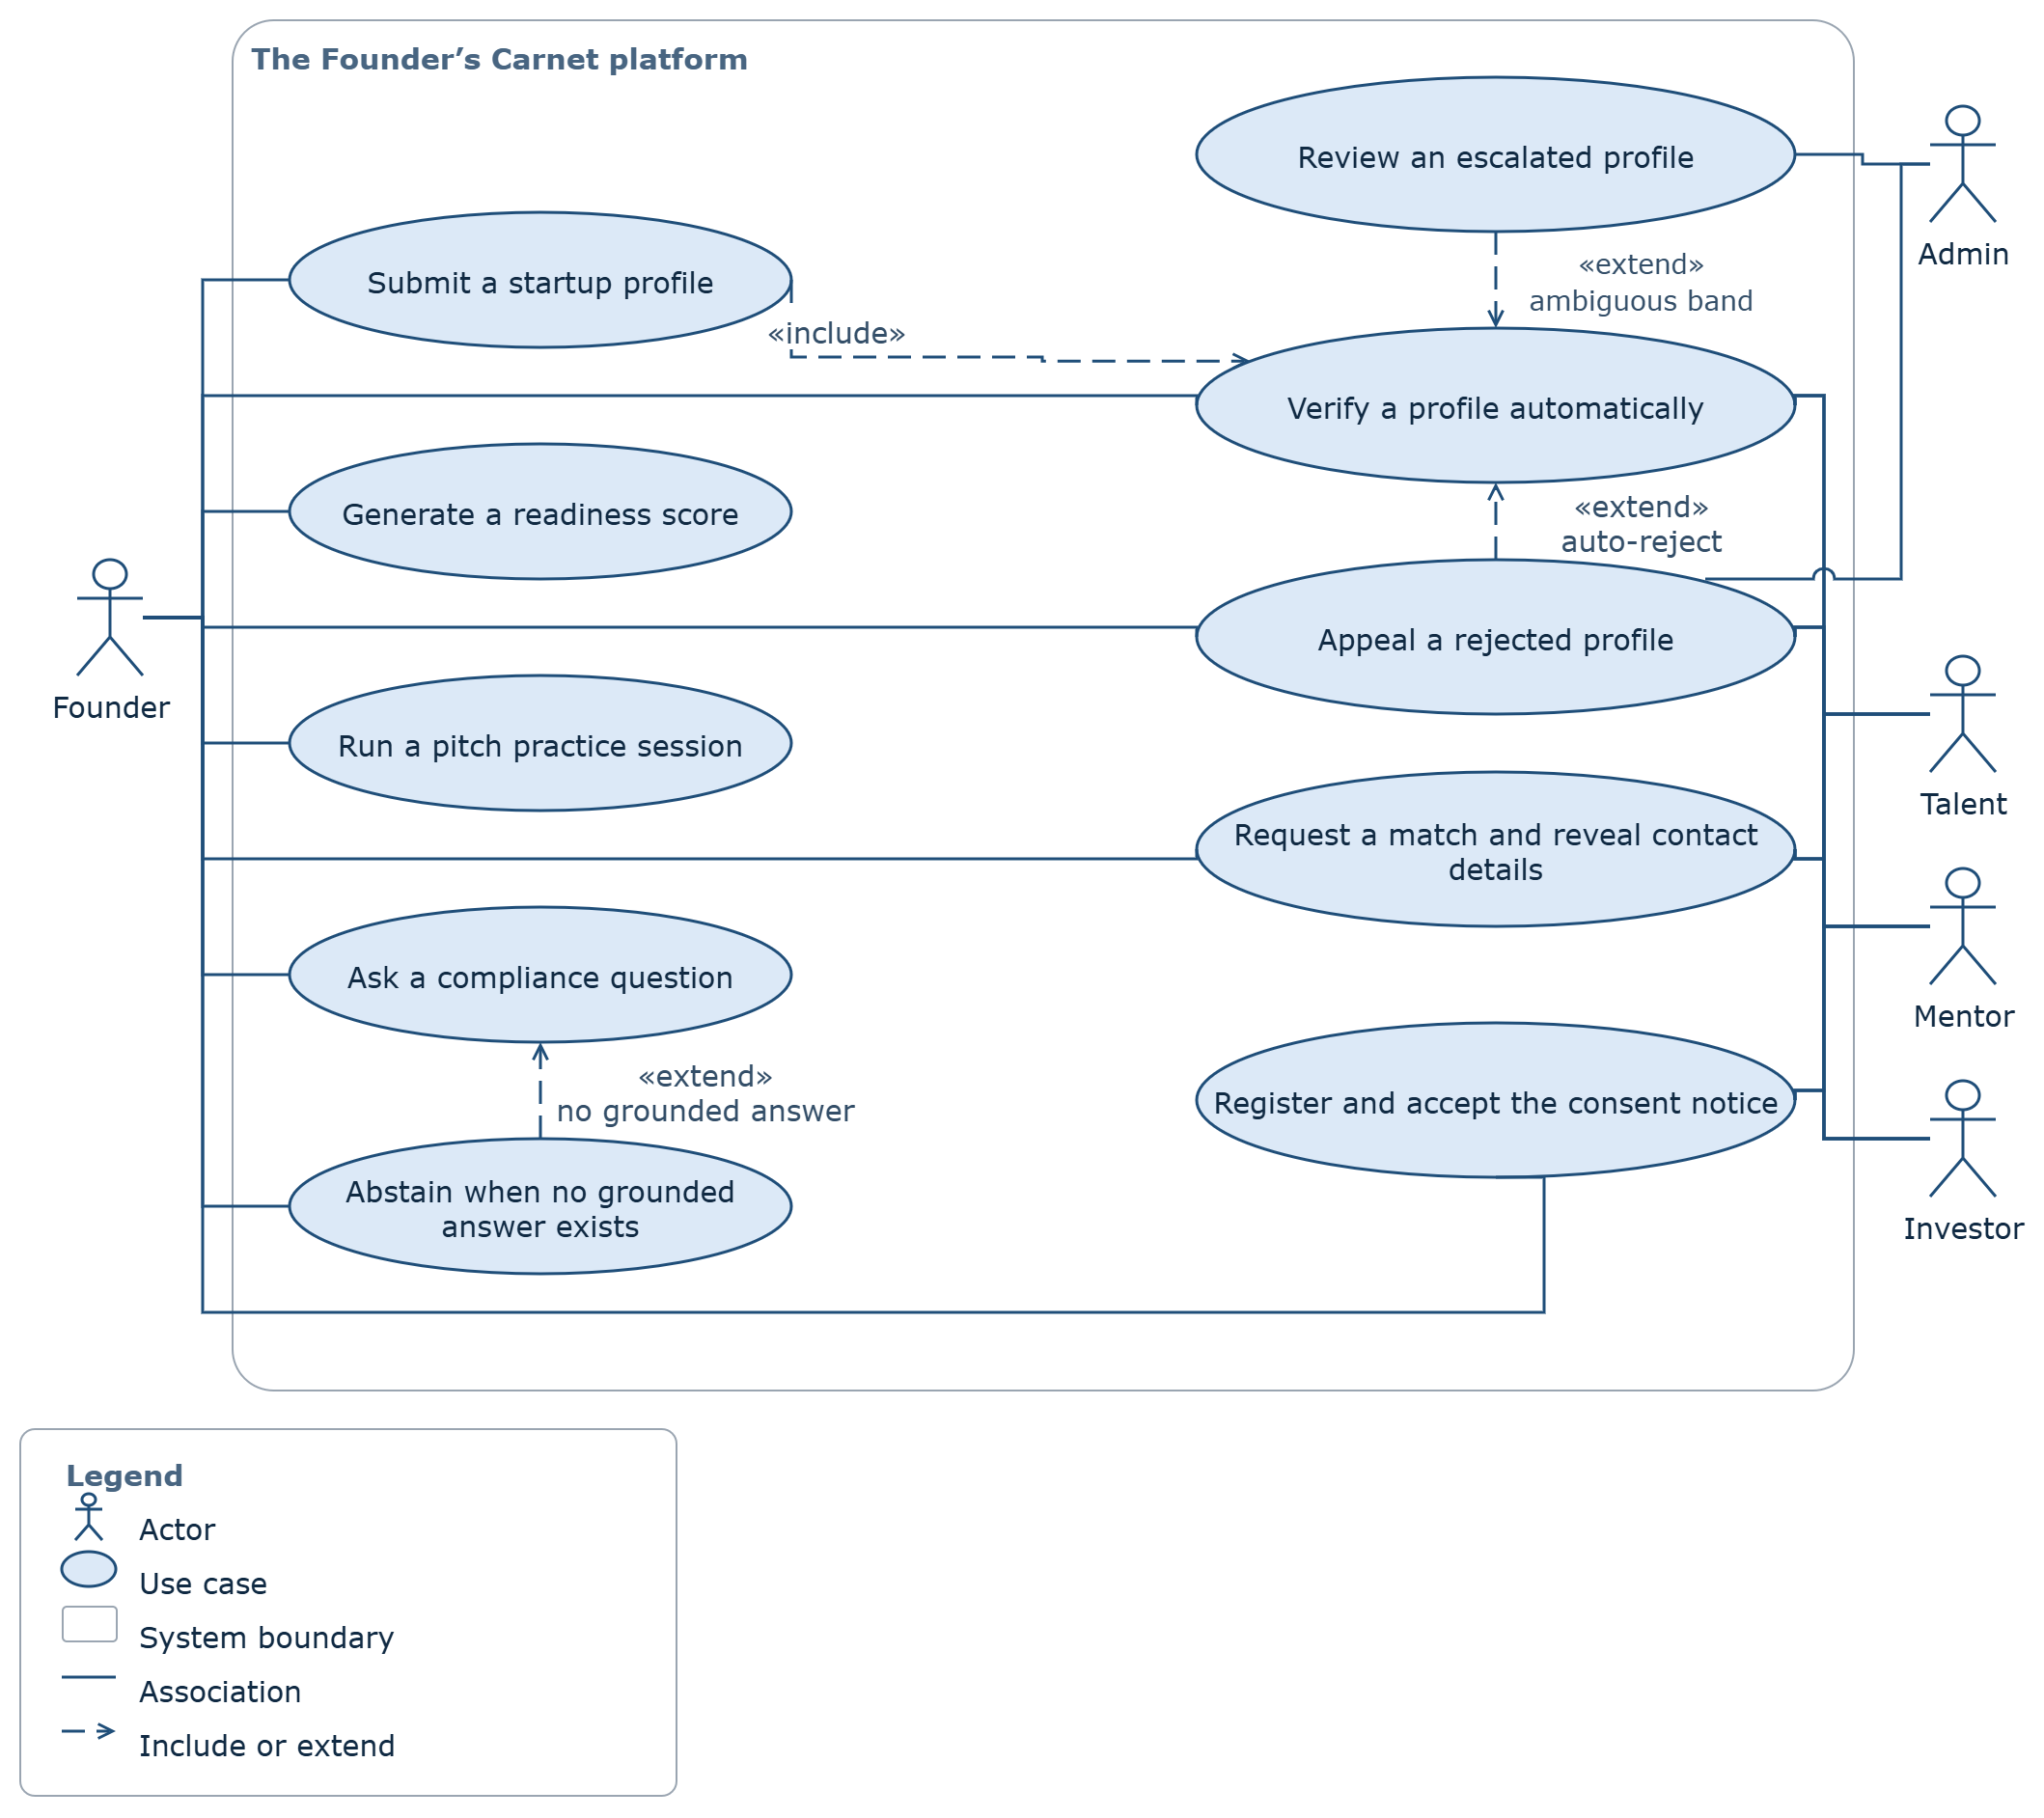
\includegraphics[width=0.6\textwidth]{Figures/fig12_use_case.png}
    \caption{Use cases and actors of The Founder's Carnet}
    \label{fig:usecases}
    \capdesc{The ten use cases and five actors.}
\end{figure}


\section{Hardware and Software Requirements}
This section lists the hardware and software needed to build and deploy the project.

\subsection{Hardware Requirements}
A laptop with a four core processor, 8~GB of RAM (16~GB recommended) and 25~GB of free disk can run the whole system. We do not need a local GPU. Embedding the regulatory documents and training the re-ranker in FYP-2 run on Google Colab. In deployment, each service runs in its own managed container with about one shared vCPU and 512~MB to 1~GB of RAM. The database is a managed PostgreSQL instance with 1~GB of storage. This fits the seeded demonstration dataset and the user target in Section~\ref{sec:nfr}. The API keeps no session state (NFR-21), so we can add more instances later.

\subsection{Software Requirements}
The software used to build and run the system is listed below. The pinned versions are in the repository.
\begin{itemize}
\item Next.js, React and TypeScript on Node.js 24 for the frontend
\item Tailwind CSS and shadcn/ui for the interface
\item Python 3.11 and FastAPI for the backend
\item PostgreSQL 16 with pgvector for the database
\item Celery and Redis for background jobs
\item sentence-transformers and scikit-learn for embeddings and the re-ranker
\item Gemini through Google AI Studio for the language model features
\item Docker, Git, GitHub Actions and pytest for containers, version control and checks
\item Vercel for the frontend, and Railway or Render for the backend and workers
\item Firecrawl and Playwright for collecting public web data (public sources only, no personal profiles)
\item Google Colab for GPU work
\end{itemize}


\providecommand{\guishots}[3]{%
  \begin{minipage}[t]{0.43\textwidth}\centering
    {\setlength{\fboxsep}{0pt}\fbox{\includegraphics[width=\linewidth]{#1}}}\\[3pt]
    {\footnotesize #2\\ #3}
  \end{minipage}}
\providecommand{\guishot}[3]{%
  \begin{minipage}[t]{0.45\textwidth}\centering
    {\setlength{\fboxsep}{0pt}\fbox{\includegraphics[width=\linewidth]{#1}}}\\[3pt]
    {\footnotesize #2\\ #3}
  \end{minipage}}

\section{Graphical User Interface (GUI)}
\label{sec:gui}
The platform has five user types: founder, talent, mentor, investor and admin. Everyone opens the authentication screen first and then lands on a dashboard for their role. This section shows 12 prototype screens with sample data. The tag under each screenshot names the use case or requirement it covers, and each user type has a navigation flow figure. Ten screens are not built yet and will be added in D3. The prototype also leaves out market research (FR-4), usage guides (FR-18), job listing management (FR-24) and consent and account deletion (FR-27), which Section~\ref{sec:fr} specifies.

\subsection{Authentication and appeal}
The authentication screen (Figure~\ref{fig:gui-common}) has a Login tab and a Register tab, with LinkedIn sign-in as an alternative. The role list does not offer admin. The user must tick the consent box before the account is created (FR-17). The Appeal form opens from the Profile screen of a user whose profile was rejected automatically. The user submits text evidence for human review. A profile can be appealed once, and a reviewer's rejection is final (FR-21). All four registered user types use the same form, and its screen is added in D3.

\begin{figure}[H]
\centering
\guishot{Figures/gui/auth.png}{Authentication}{Register and accept the consent notice; FR-17, FR-22}
{\caption{\label{fig:gui-common}\textbf{Authentication screen.}}}
\capdesc{All users share this login screen, and it shows the consent notice before an account is created.}
\end{figure}

\Needspace{14\baselineskip}
\subsection{Founder}
After login, the founder lands on the dashboard (Figure~\ref{fig:gui-founder-1}a), where a banner shows the verification status. The sidebar is in Figure~\ref{fig:nav-founder}. A rejected profile links to the Appeal form (Figure~\ref{fig:gui-founder-1}b). The Readiness score shows seven dimension scores and one overall score (Figure~\ref{fig:gui-founder-1}c). From there the founder can recalculate or start pitch practice, picking an investor persona and chatting with a simulated investor (Figure~\ref{fig:gui-founder-1}d). When the chat ends, the Session feedback screen shows feedback and next steps (Figure~\ref{fig:gui-founder-2}a). Matches can be filtered by role, sector and stage (Figure~\ref{fig:gui-founder-2}b). Contact details stay locked until a request is accepted. For now, ranking uses embedding similarity, and the re-ranker comes in the second semester. The compliance assistant opens as a panel on any screen. It answers in English with sources and dates, or says it has no grounded answer. Its screen is added in D3.

\begin{figure}[H]
\centering
\guishots{Figures/gui/founder_dashboard.png}{(a) Dashboard}{Verification status shown; FR-15}\hfill
\guishots{Figures/gui/founder_profile.png}{(b) Profile}{Submit a startup profile; FR-1, FR-14, FR-15}\\[6pt]
\guishots{Figures/gui/founder_readiness.png}{(c) Readiness score}{Generate a readiness score; FR-2}\hfill
\guishots{Figures/gui/founder_pitch.png}{(d) Pitch practice}{Run a pitch practice session; FR-3}
{\caption{\label{fig:gui-founder-1}\textbf{Founder screens: dashboard, profile, readiness score and pitch practice.}}}
\capdesc{Founder screens with sample data, tagged with the use case or requirement each one covers.}
\end{figure}

\begin{figure}[H]
\centering
\guishots{Figures/gui/founder_feedback.png}{(a) Session feedback}{Run a pitch practice session; FR-3}\hfill
\guishots{Figures/gui/founder_matches.png}{(b) Matches}{Request a match and reveal contact details; FR-7}
{\caption{\label{fig:gui-founder-2}\textbf{Founder screens: session feedback and matches.}}}
\capdesc{Founder screens with sample data, tagged with the use case or requirement each one covers.}
\end{figure}

\begin{figure}[H]
\centering
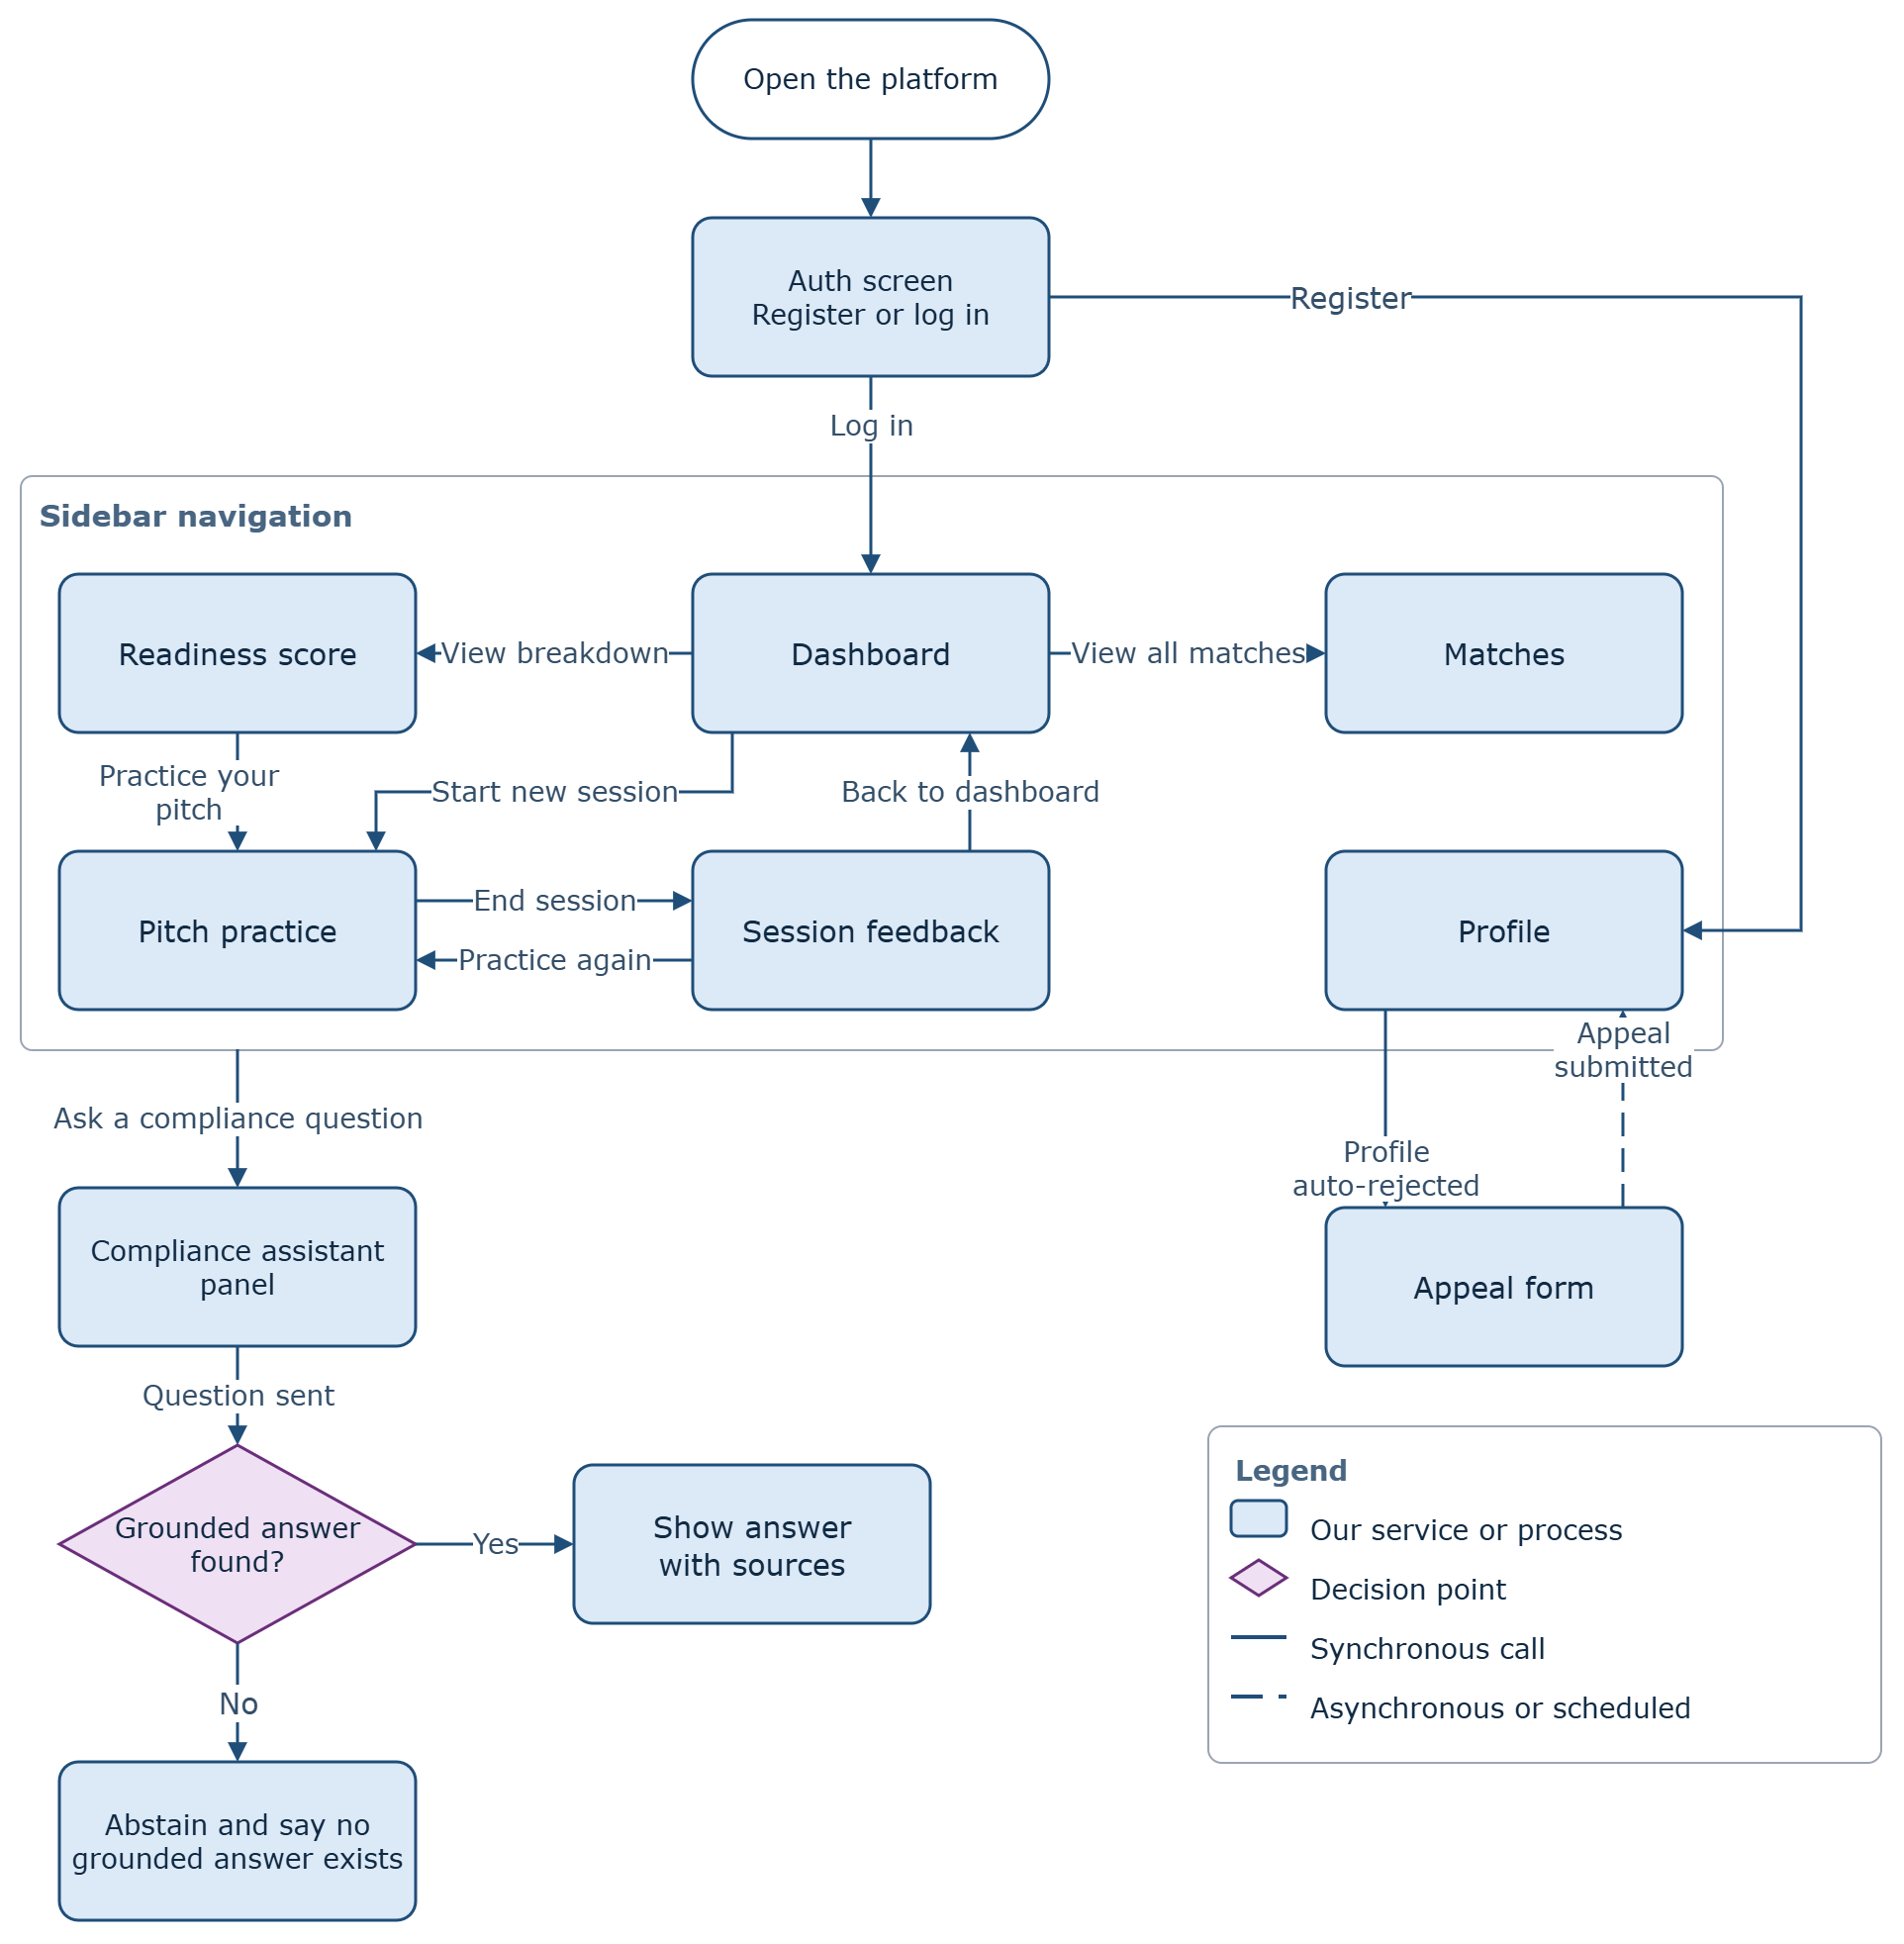
\includegraphics[width=0.6\textwidth]{Figures/fig07_nav_founder.png}
{\caption{\label{fig:nav-founder}\textbf{Navigation flow for the founder role.}}}
\capdesc{Founders move between screens from sidebar, reach appeal form and compliance assistant from actions.}
\end{figure}

\Needspace{14\baselineskip}
\subsection{Talent}
The talent dashboard and Job board are in Figure~\ref{fig:gui-talent}, and the sidebar is in Figure~\ref{fig:nav-talent}. The Profile, Resume optimizer and Matches screens are added in D3. The Profile screen links an automatically rejected profile to the Appeal form. Resume optimizer shows the suggested changes next to original, and it is part of paid tier. On the Matches screen, contact details stay locked until other side accepts.

\begin{figure}[H]
\centering
\guishot{Figures/gui/talent_dashboard.png}{(a) Dashboard}{Overview of talent features}\hfill
\guishot{Figures/gui/talent_jobs.png}{(b) Job board}{Job and internship listings; FR-6, FR-25}
{\caption{\label{fig:gui-talent}\textbf{Talent screens: dashboard and job board.}}}
\capdesc{Talent screens with sample data, tagged with the use case or requirement each one covers.}
\end{figure}

\begin{figure}[H]
\centering
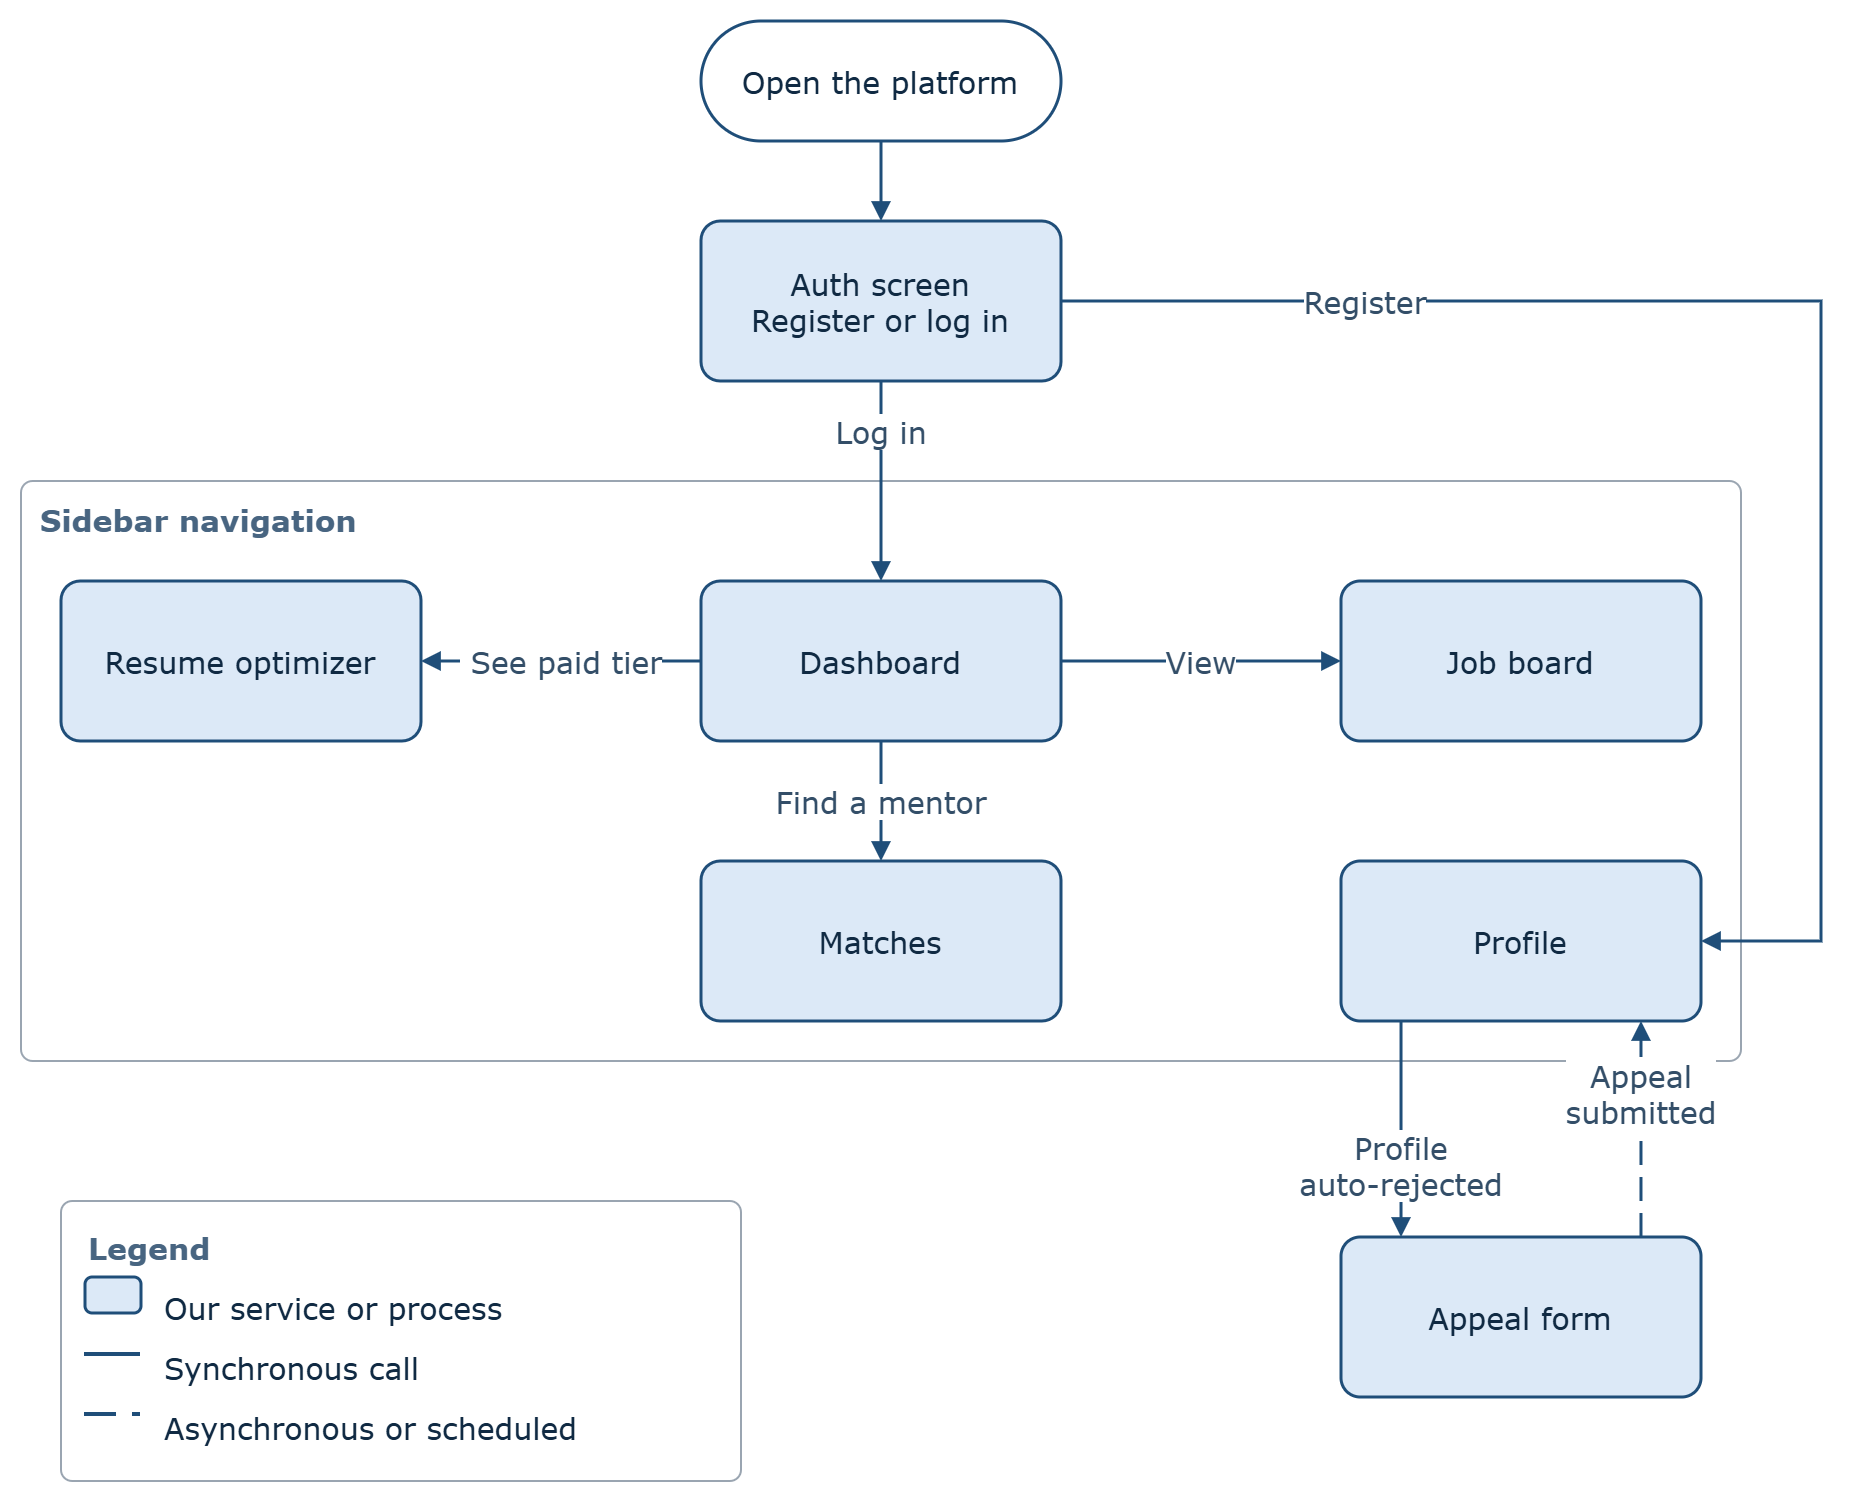
\includegraphics[width=0.6\textwidth]{Figures/fig08_nav_talent.png}
{\caption{\label{fig:nav-talent}\textbf{Navigation flow for the talent role.}}}
\capdesc{Talent users open resume optimizer, job board and mentor matches from sidebar, and can appeal a rejected profile.}
\end{figure}

\Needspace{14\baselineskip}
\subsection{Mentor}
The mentor dashboard (Figure~\ref{fig:gui-mentor}) has an availability toggle and Accept and Decline buttons for pending requests. The sidebar is in Figure~\ref{fig:nav-mentor}. The Profile and Requests screens are added in D3. The Profile screen holds the expertise and availability details. On the Requests screen, accepting a request activates the match and reveals contact details, and declining closes the request.

\begin{figure}[H]
\centering
\guishot{Figures/gui/mentor_dashboard.png}{Dashboard}{Overview of mentor features}
{\caption{\label{fig:gui-mentor}\textbf{Mentor dashboard.}}}
\capdesc{Screen of the mentor interface with sample data. The tag names the feature the screen covers.}
\end{figure}

\begin{figure}[H]
\centering
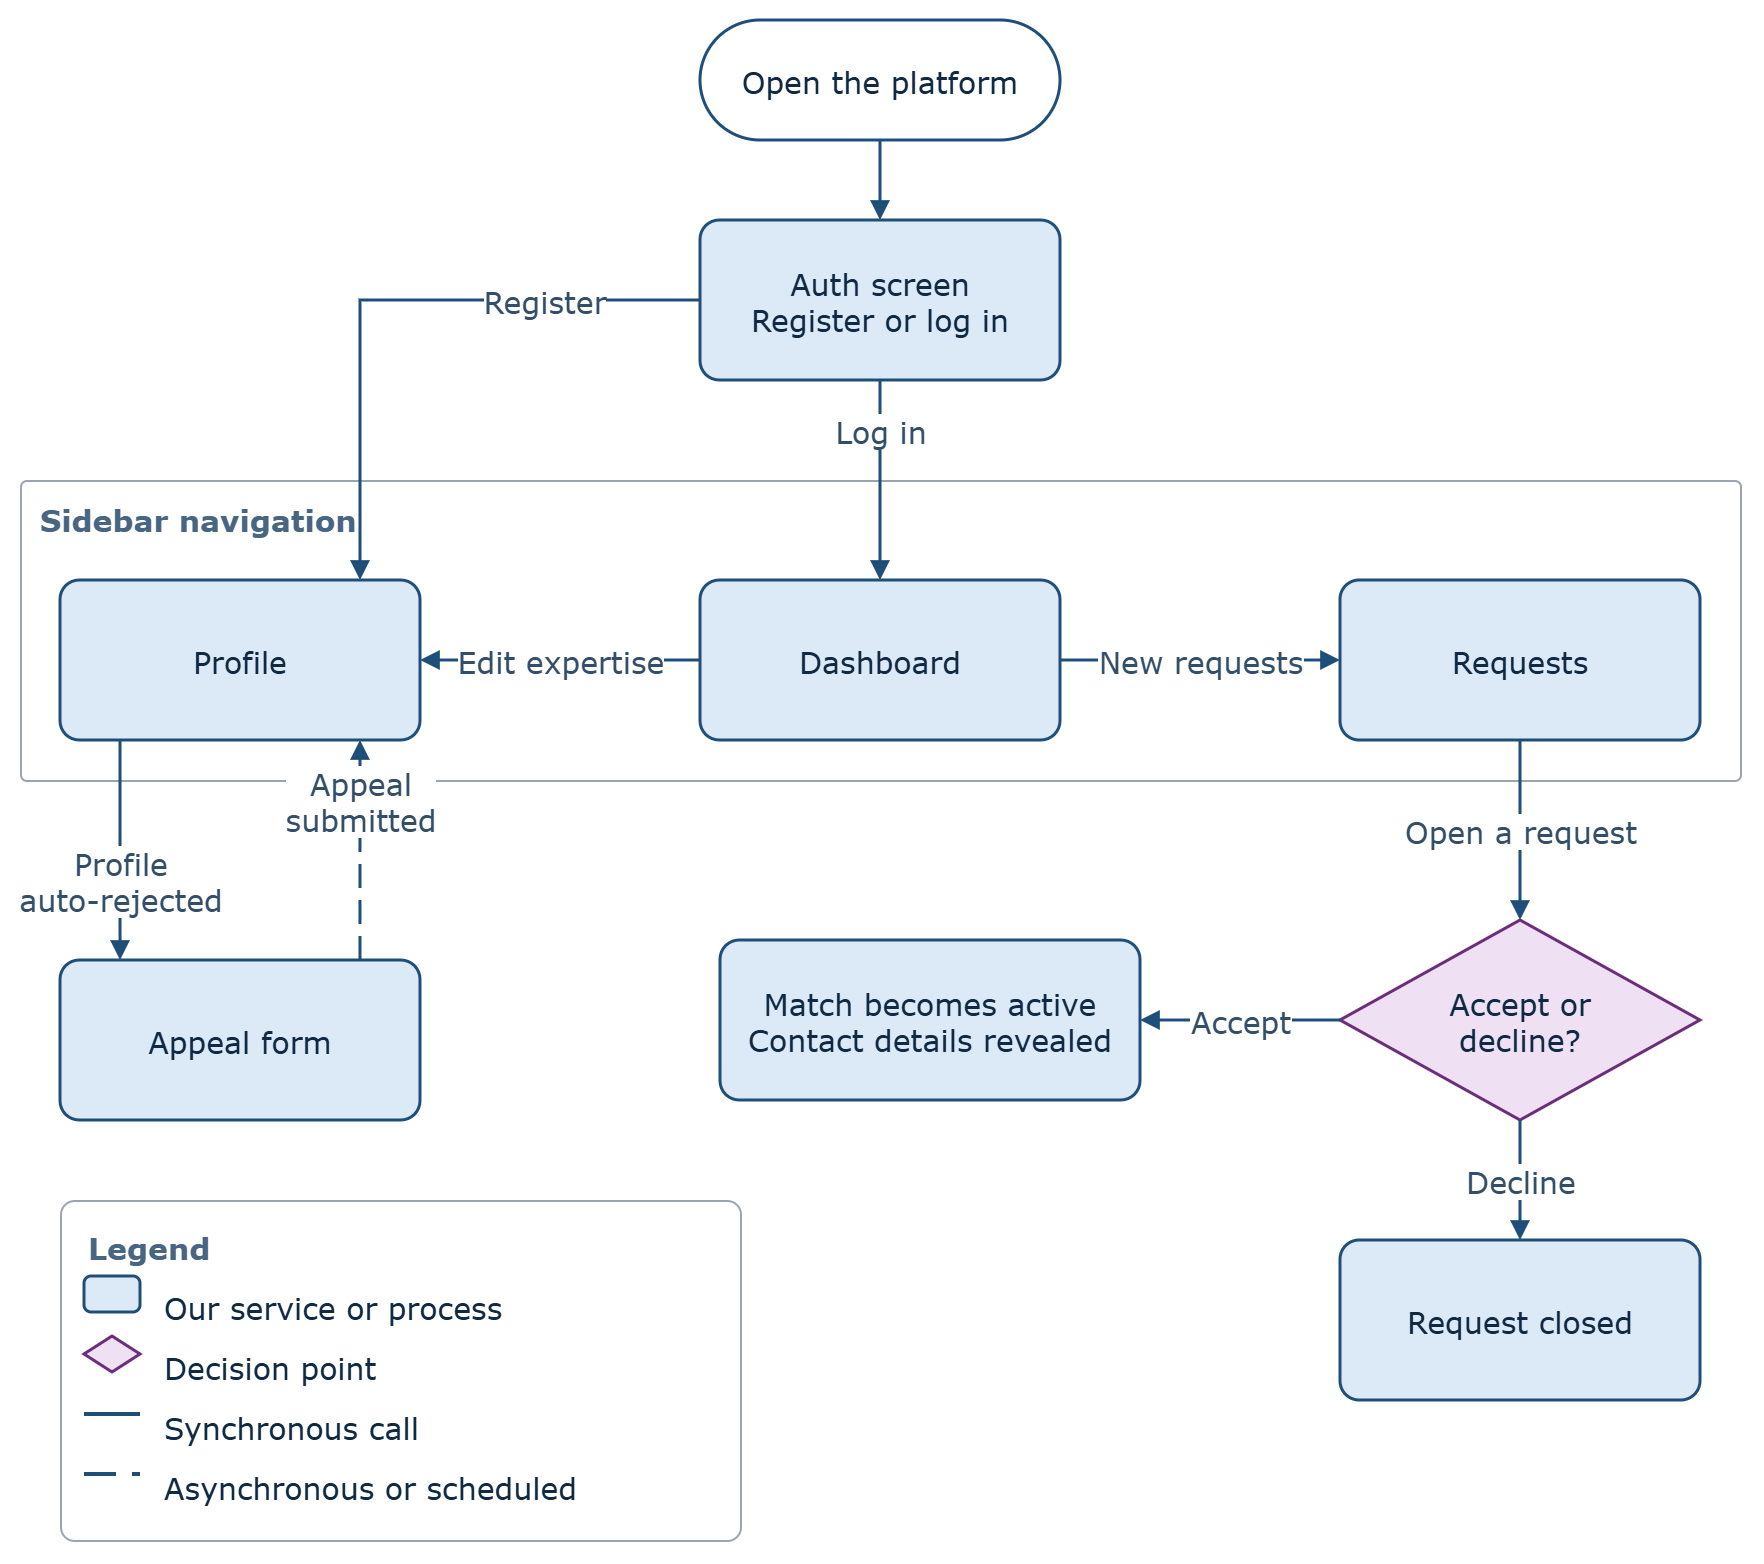
\includegraphics[width=0.6\textwidth]{Figures/fig09_nav_mentor.png}
{\caption{\label{fig:nav-mentor}\textbf{Navigation flow for the mentor role.}}}
\capdesc{Mentors manage requests from dashboard, where accepting a request reveals contact details and declining closes it.}
\end{figure}

\Needspace{14\baselineskip}
\subsection{Investor}
The investor dashboard (Figure~\ref{fig:gui-investor}) has View founder and Request match buttons on each recommended founder. The sidebar is in Figure~\ref{fig:nav-investor}. The Profile, Founders and Requests screens are added in D3. Founders lists only verified startups with a completed readiness assessment (FR-10). The readiness score is shown as information and does not filter the list. Requests tracks the match requests the investor has sent.

\begin{figure}[H]
\centering
\guishot{Figures/gui/investor_dashboard.png}{Dashboard}{Overview of investor features}
{\caption{\label{fig:gui-investor}\textbf{Investor dashboard.}}}
\capdesc{Investor screen with sample data, tagged with the use case or requirement it covers.}
\end{figure}

\begin{figure}[H]
\centering
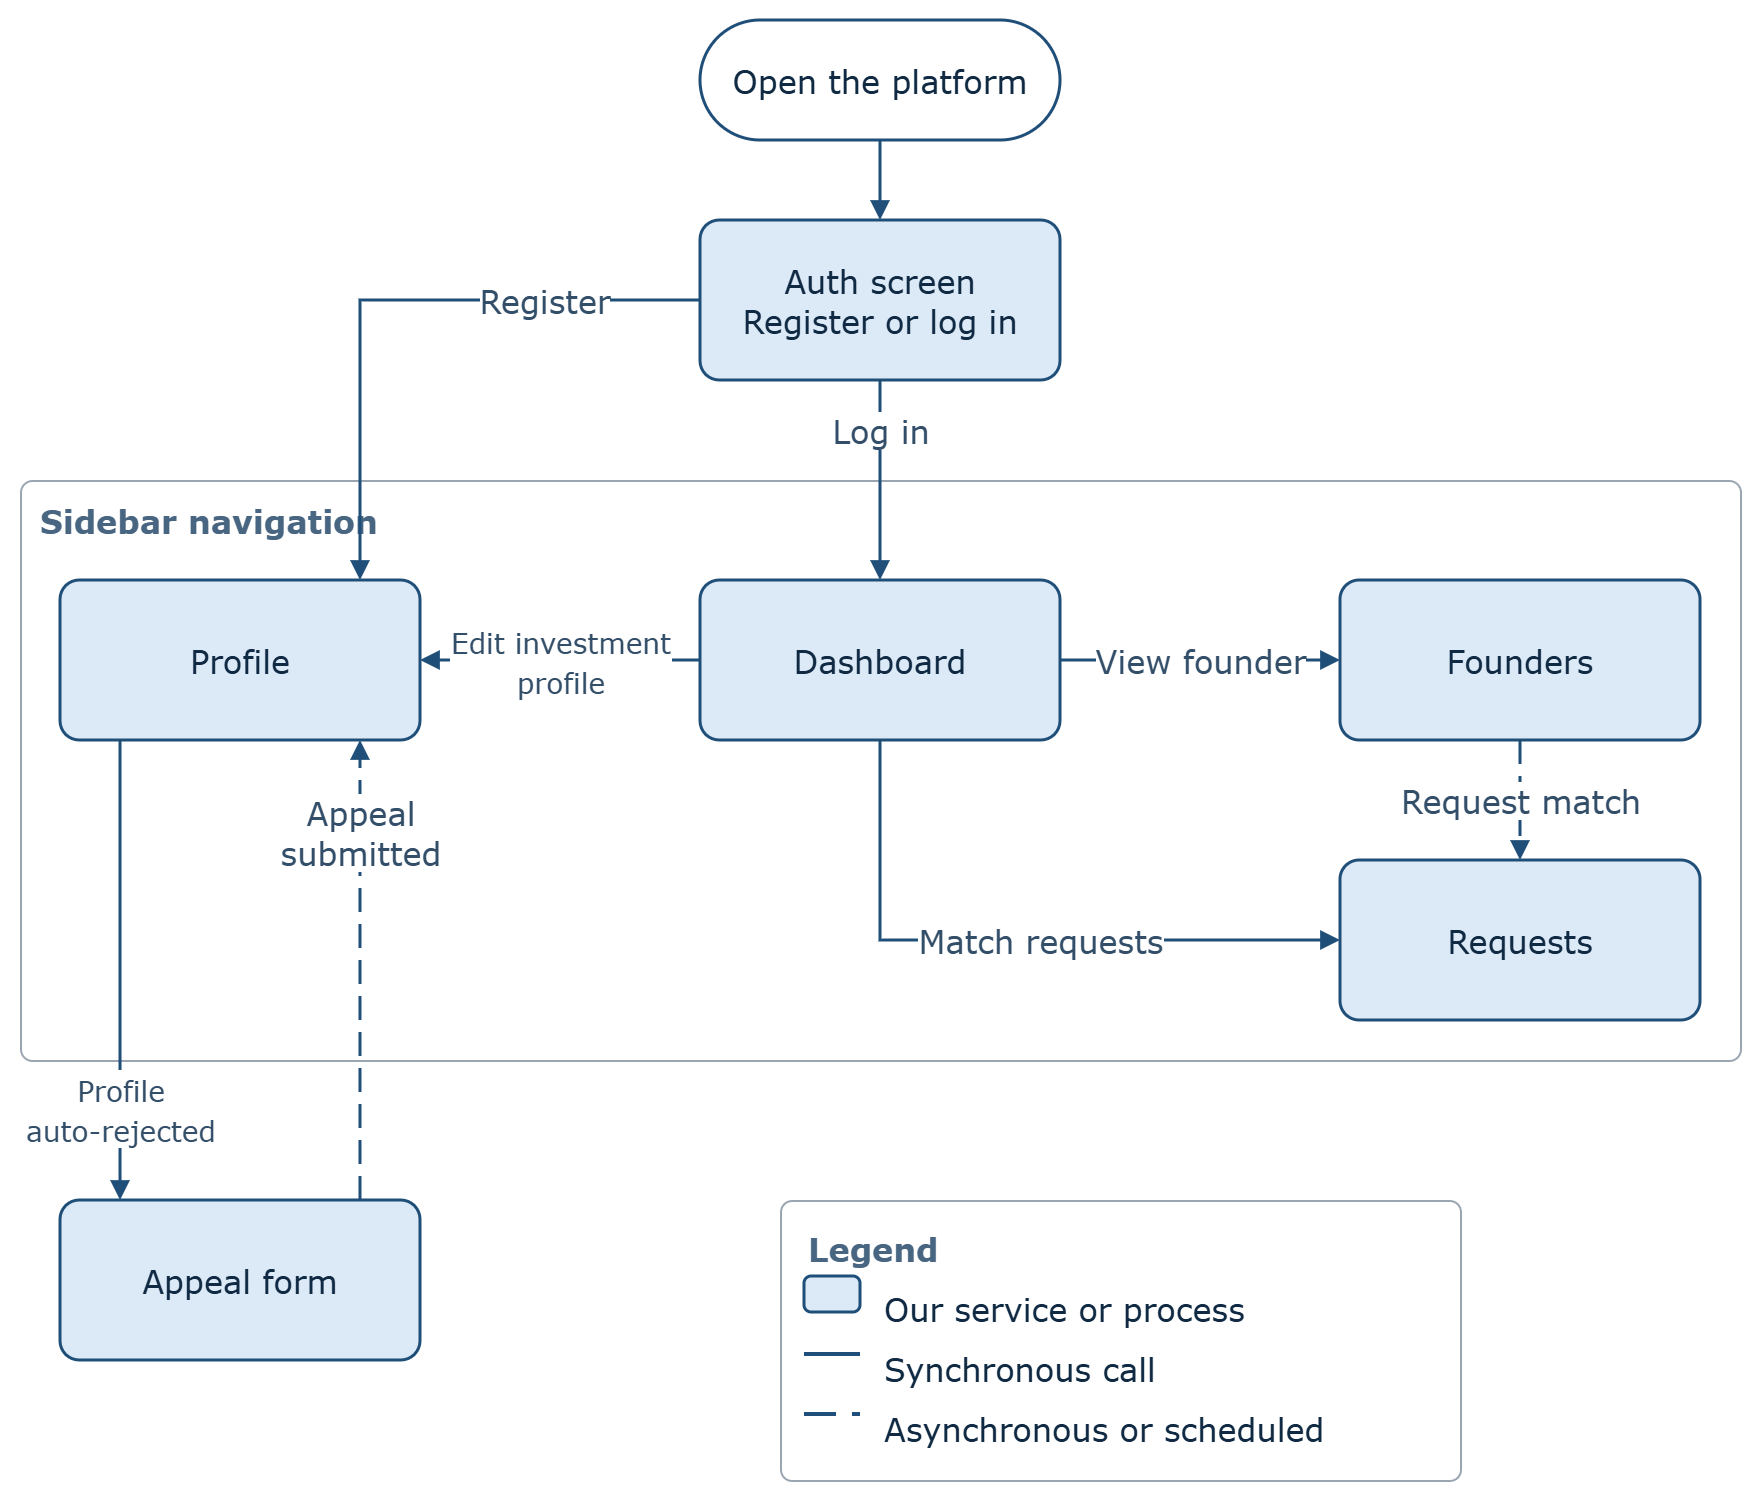
\includegraphics[width=0.6\textwidth]{Figures/fig10_nav_investor.png}
{\caption{\label{fig:nav-investor}\textbf{Navigation flow for the investor role.}}}
\capdesc{An investor browses verified startups, sends match requests and tracks them on the requests screen.}
\end{figure}

\Needspace{14\baselineskip}
\subsection{Admin}
The admin signs in with Login only and lands on the console (Figure~\ref{fig:gui-admin}). It is the only item in the admin sidebar (Figure~\ref{fig:nav-admin}). The review queue holds two kinds of cases: profiles escalated because automatic verification was unclear, and appeals of rejected profiles. The admin approves or rejects each one, and a rejection is final (FR-26).

\begin{figure}[H]
\centering
\guishot{Figures/gui/admin_console.png}{Admin console}{Review an escalated profile; Appeal a rejected profile; FR-26}
{\caption{\label{fig:gui-admin}\textbf{Admin console.}}}
\capdesc{The review queue where an admin decides on escalated profiles and appeals.}
\end{figure}

\begin{figure}[H]
\centering
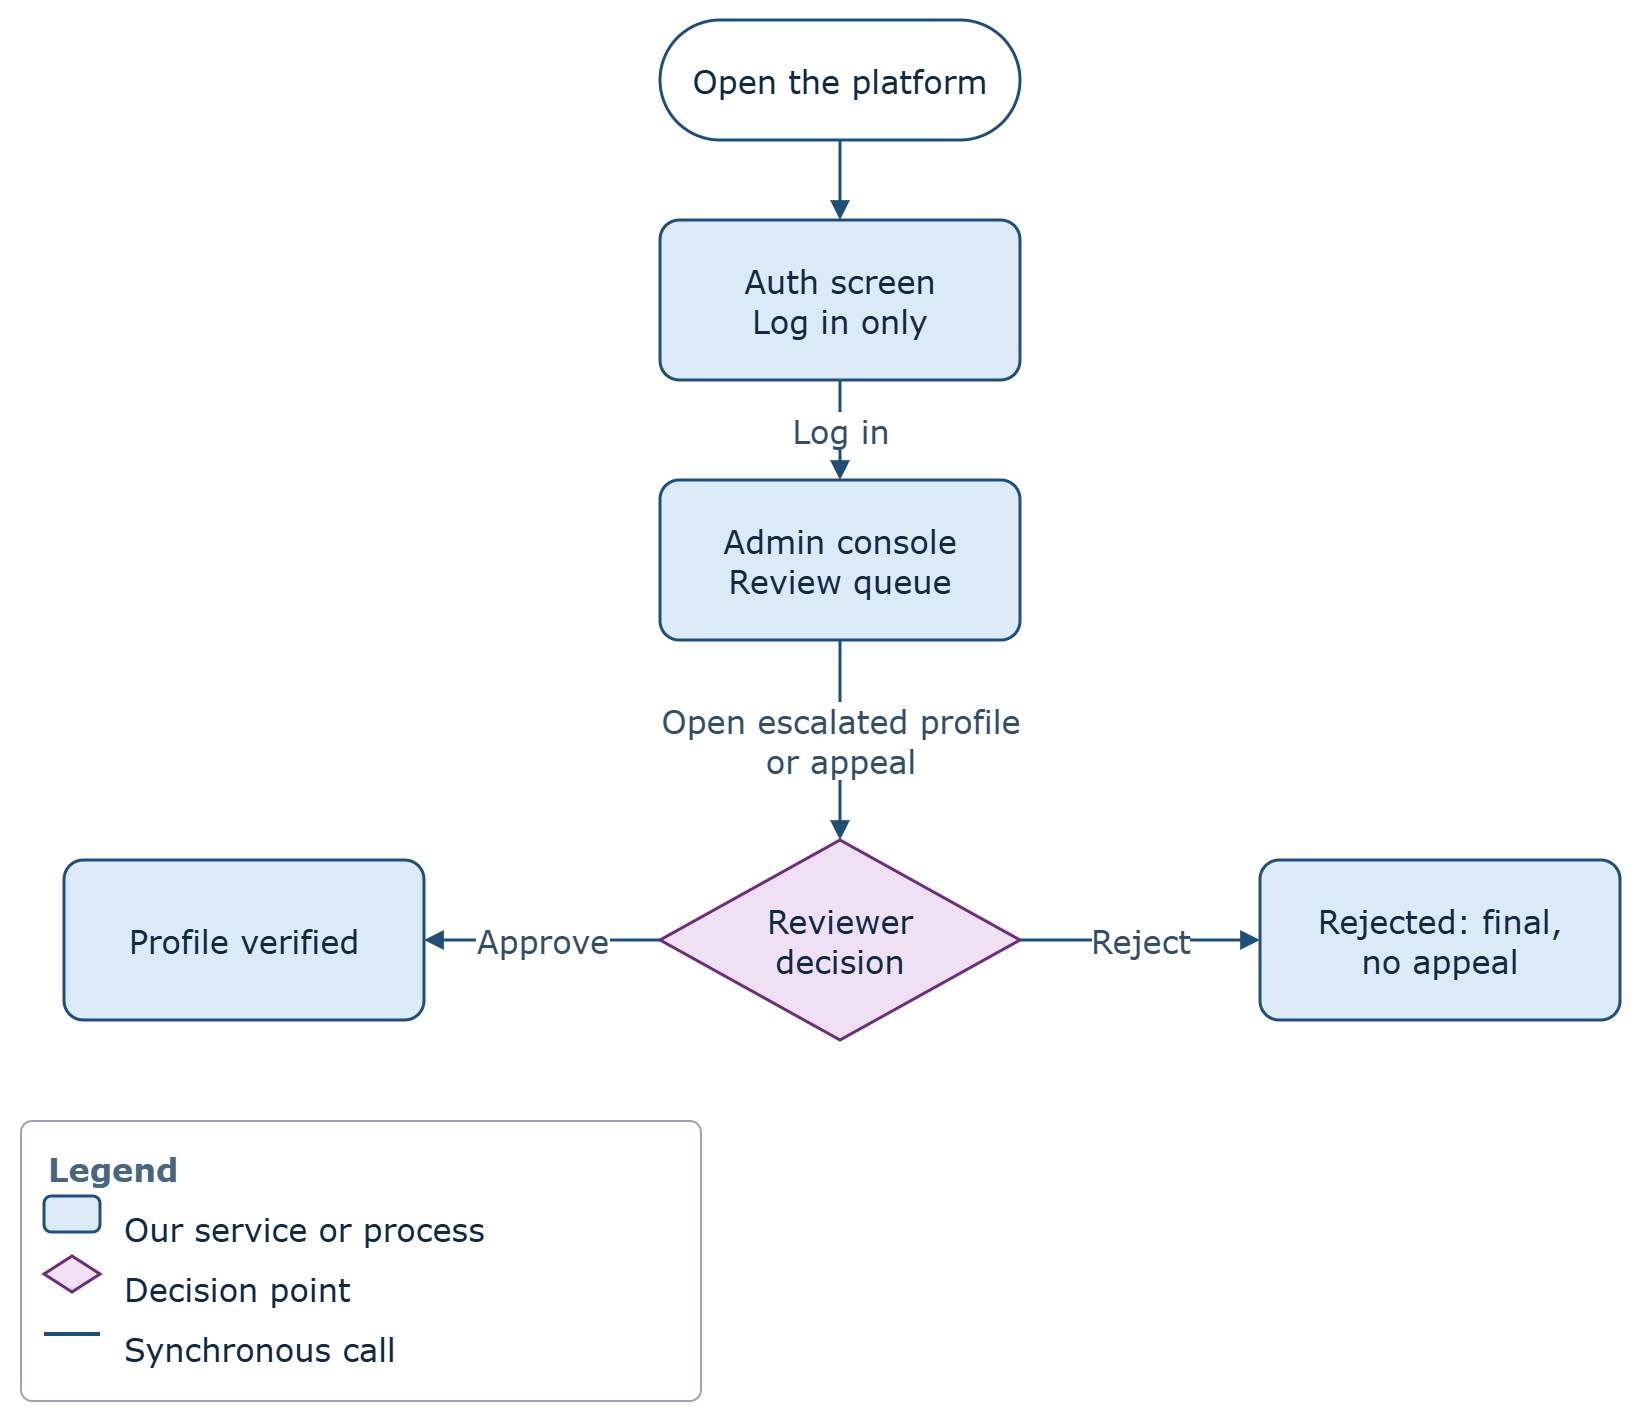
\includegraphics[width=0.6\textwidth]{Figures/fig11_nav_admin.png}
{\caption{\label{fig:nav-admin}\textbf{Navigation flow for the admin role.}}}
\capdesc{The admin opens the review queue, approves or rejects each escalated profile or appeal and rejection is final.}
\end{figure}


\section{Database Design}\label{sec:db}
The system stores its data in PostgreSQL. The current schema has 41 tables in five modules, and tables deferred to FYP-2 are drawn in gray and tagged. The table and attribute counts are planning figures and may change when the schema is built, under the policy in Section~\ref{sec:dbchange}.

\Needspace{14\baselineskip}
\subsection{Entity-Relationship (ER) Diagram}
Figure~\ref{fig:er-overview} shows all 41 tables by name in five modules. Figures~\ref{fig:er-accounts} to~\ref{fig:er-compliance} show one module each, with primary and foreign keys. Tables owned by another module appear as dashed gray boxes.

\begin{figure}[H]
    \centering
    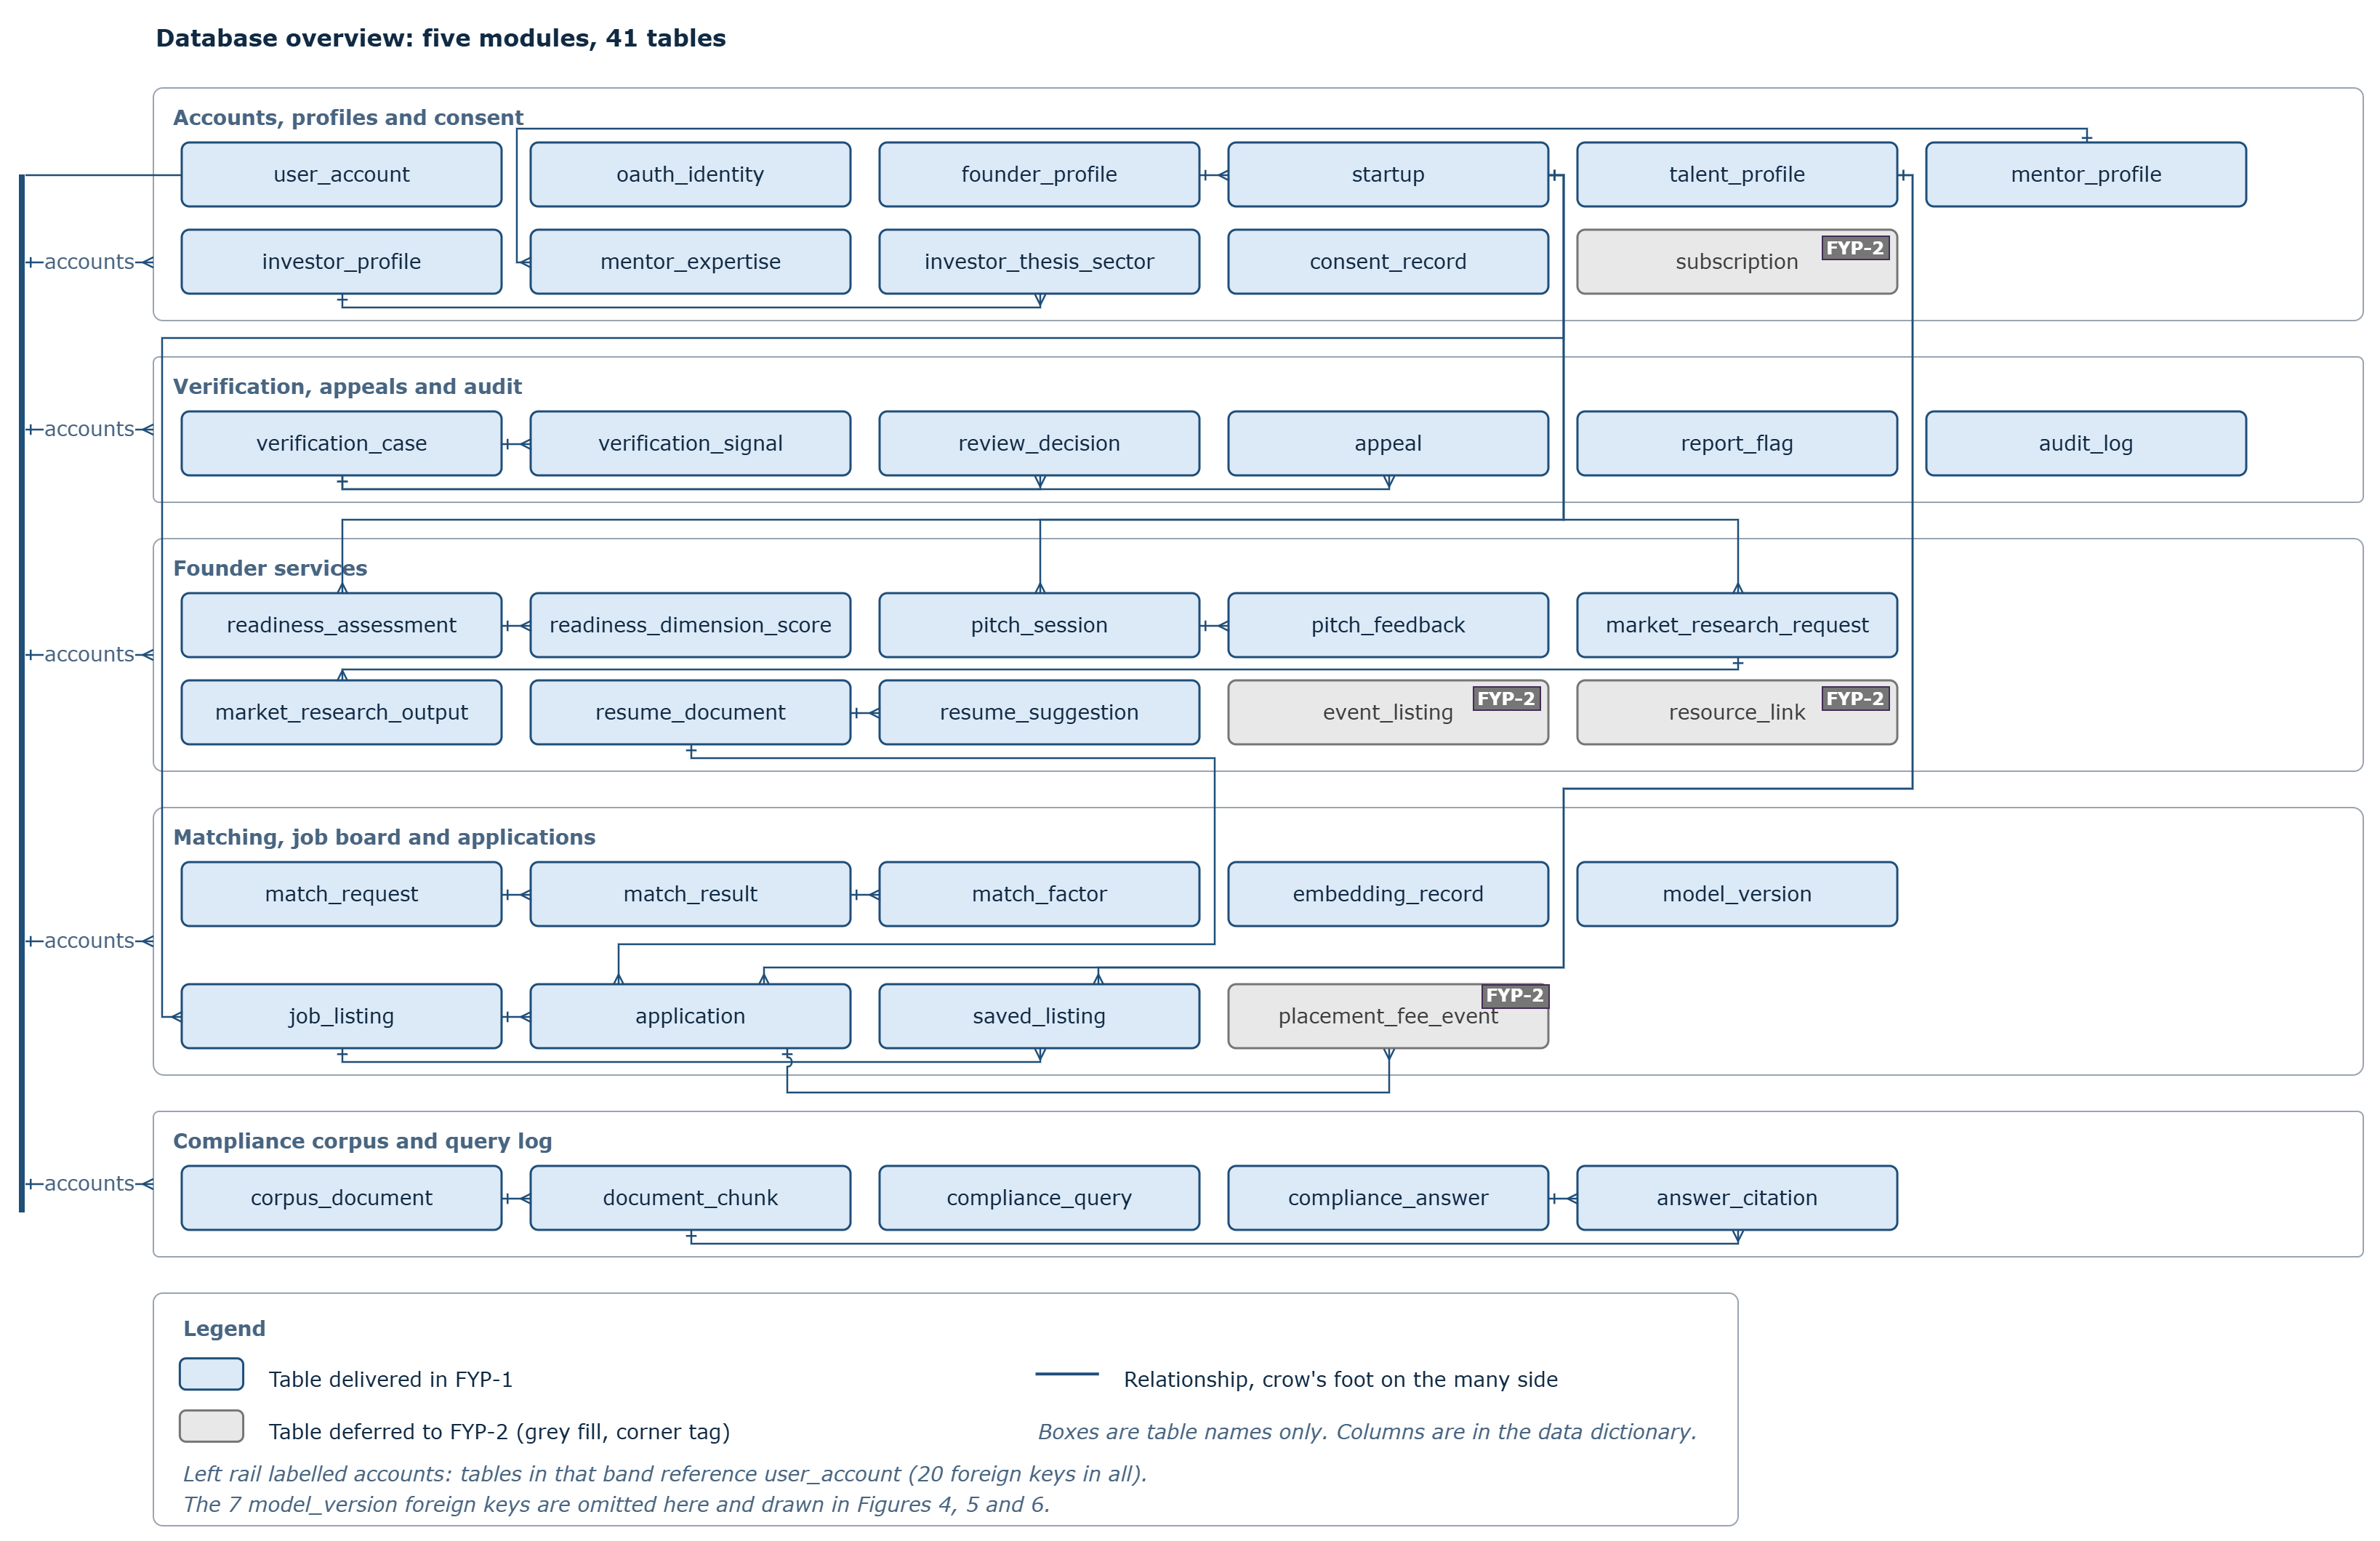
\includegraphics[width=\textwidth,height=0.36\textheight,keepaspectratio]{Figures/fig01_er_overview}
    \caption{Database overview: five modules and 41 tables}
    \label{fig:er-overview}
    \capdesc{All 41 tables grouped into five modules, shown by name only.}
\end{figure}

In Figure~\ref{fig:er-accounts}, each user has one \texttt{user\_account} row and one profile for their role. Startups belong to the founder profile because one founder can register several.

\begin{figure}[H]
    \centering
    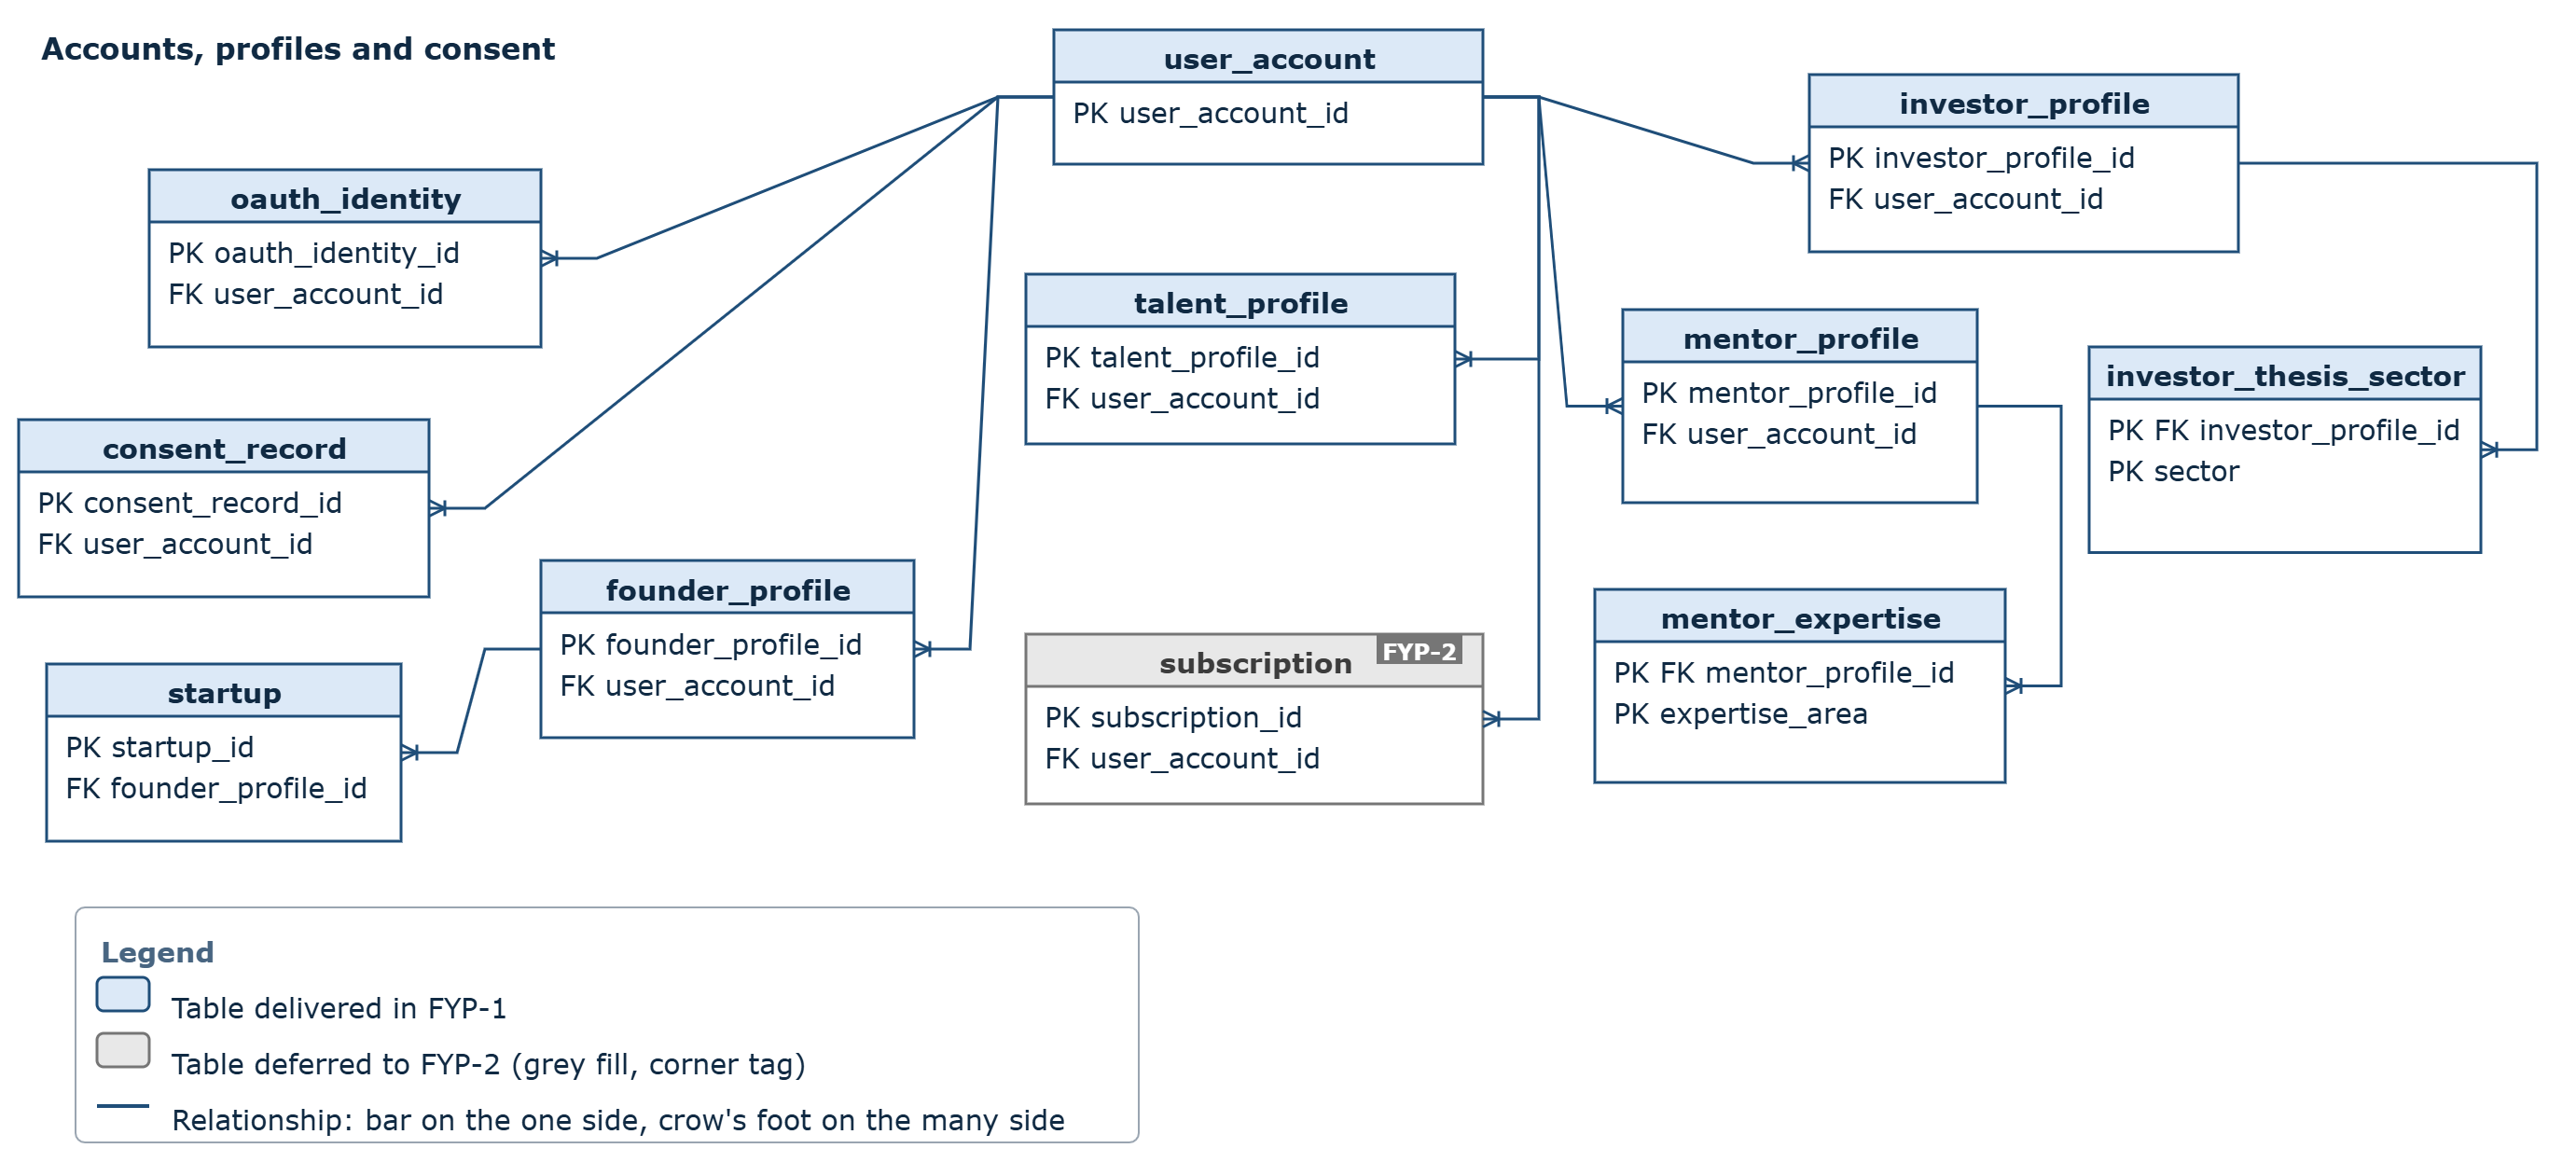
\includegraphics[width=\textwidth,height=0.36\textheight,keepaspectratio]{Figures/fig02_er_accounts}
    \caption{Accounts, profiles and consent module}
    \label{fig:er-accounts}
    \capdesc{User accounts, role profiles, startups, and consent, with keys.}
\end{figure}

In Figure~\ref{fig:er-verification}, each case stores its score, band and threshold version. This lets us explain a decision even after the thresholds change. A unique constraint allows one appeal per case.

\begin{figure}[H]
    \centering
    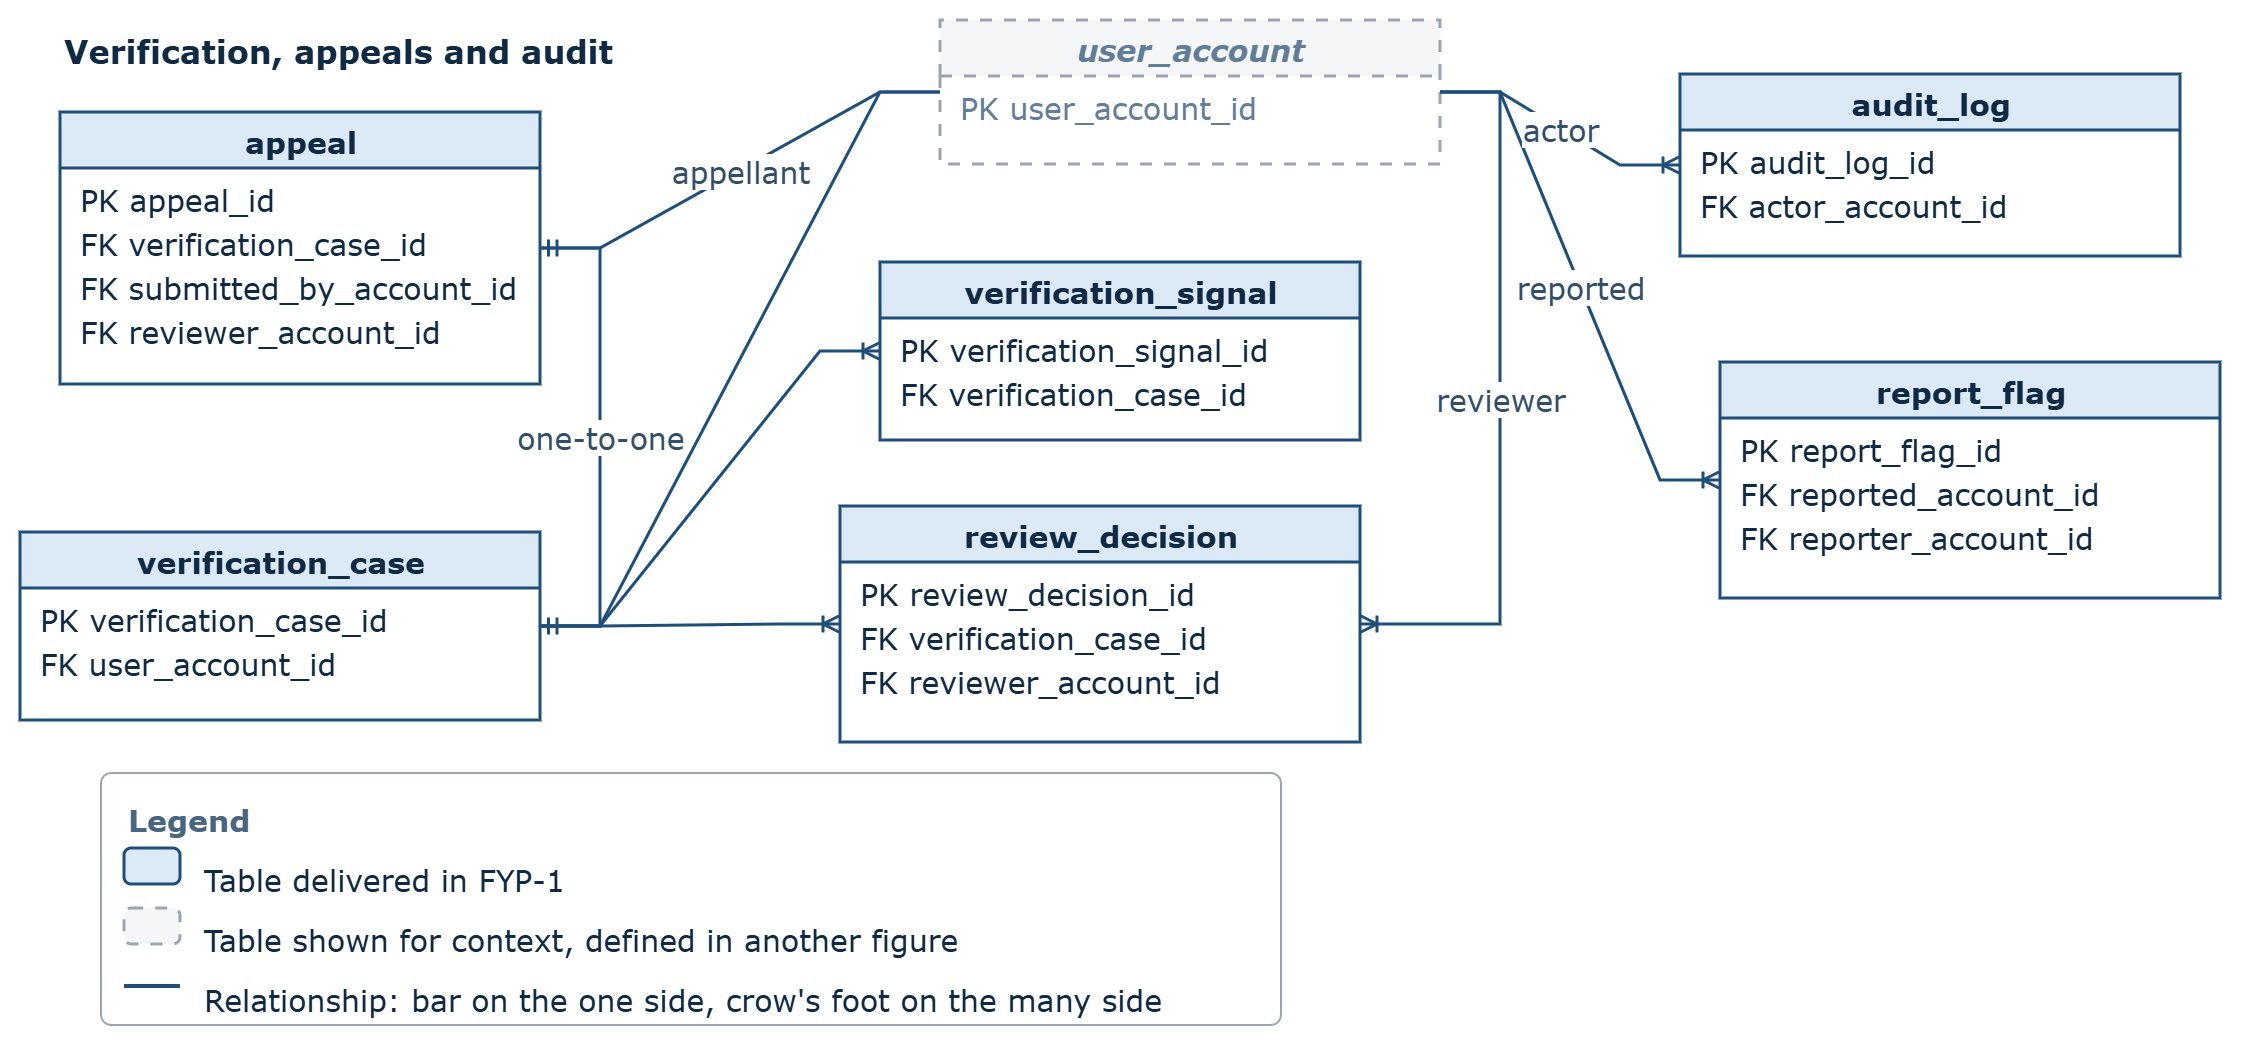
\includegraphics[width=\textwidth,height=0.36\textheight,keepaspectratio]{Figures/fig03_er_verification}
    \caption{Verification, appeals and audit module}
    \label{fig:er-verification}
    \capdesc{Verification cases, appeals, and the audit trail, with keys.}
\end{figure}

In Figure~\ref{fig:er-founder}, readiness assessments, pitch sessions, and market research outputs record the prompt and model version behind them. The evidence log described in Chapter 5 reads from these.

\begin{figure}[H]
    \centering
    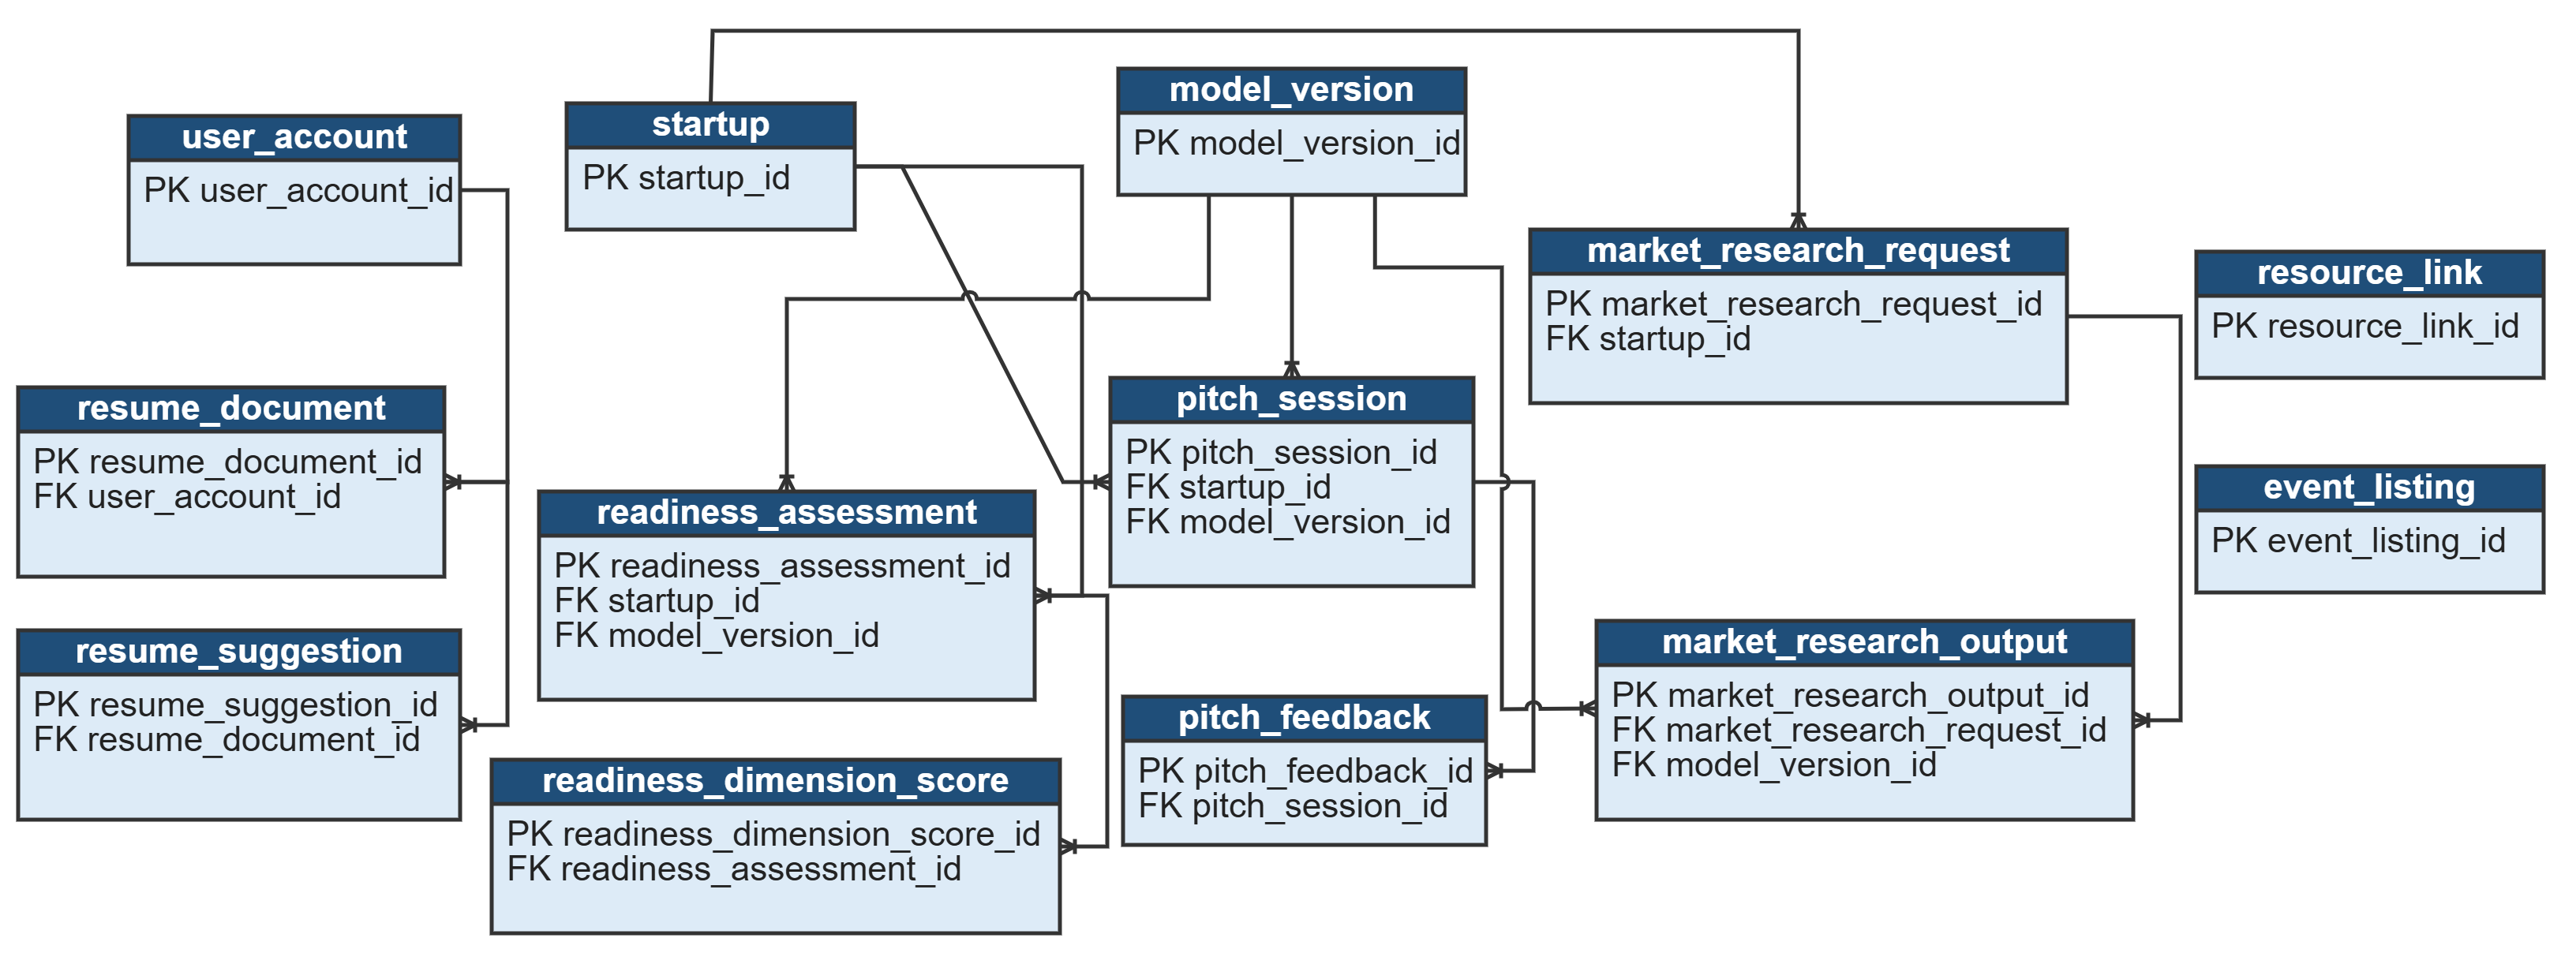
\includegraphics[width=\textwidth,height=0.36\textheight,keepaspectratio]{Figures/fig04_er_founder_services}
    \caption{Founder services module}
    \label{fig:er-founder}
    \capdesc{Readiness assessments, pitch sessions, and market research outputs, with keys.}
\end{figure}

In Figure~\ref{fig:er-matching}, each match result stores a retrieval score, a re-ranking score and its match factors. The re-ranking score stays empty until the FYP-2 re-ranker exists. The embedding table links to its owner by type and ID, without a foreign key.

\begin{figure}[H]
    \centering
    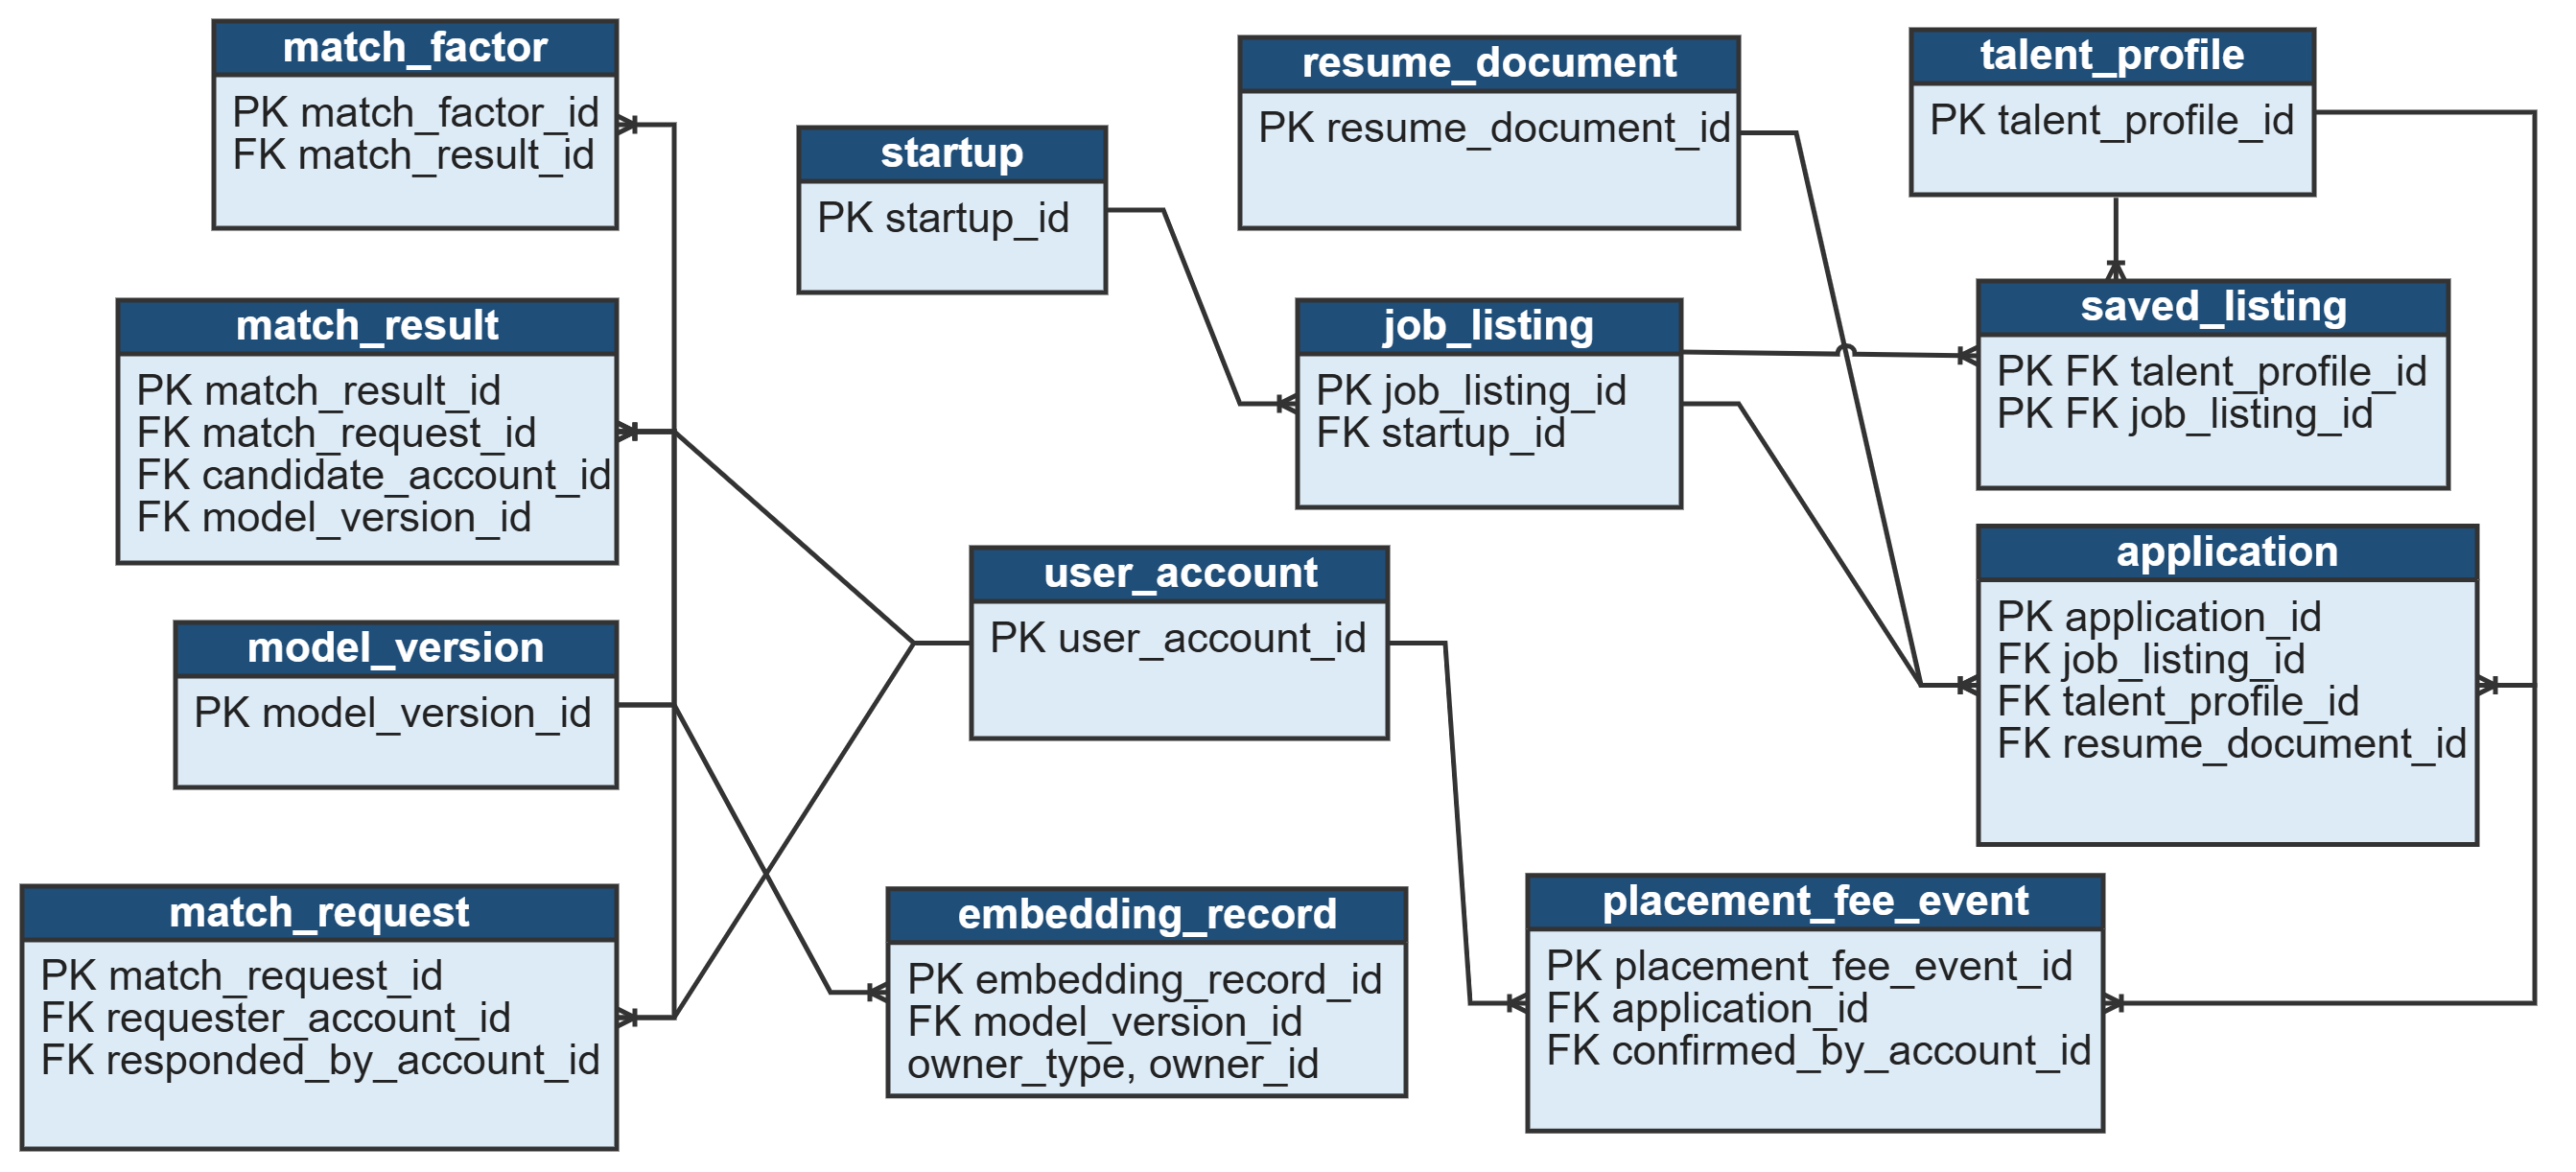
\includegraphics[width=\textwidth,height=0.36\textheight,keepaspectratio]{Figures/fig05_er_matching_jobs}
    \caption{Matching, job board and applications module}
    \label{fig:er-matching}
    \capdesc{Match results, job listings, applications, and embeddings, with keys.}
\end{figure}

In Figure~\ref{fig:er-compliance}, each source document stores its effective date, its consolidation date and its retrieval date, because these often differ for Pakistani regulations. Each answer stores whether the assistant abstained and why.

\begin{figure}[H]
    \centering
    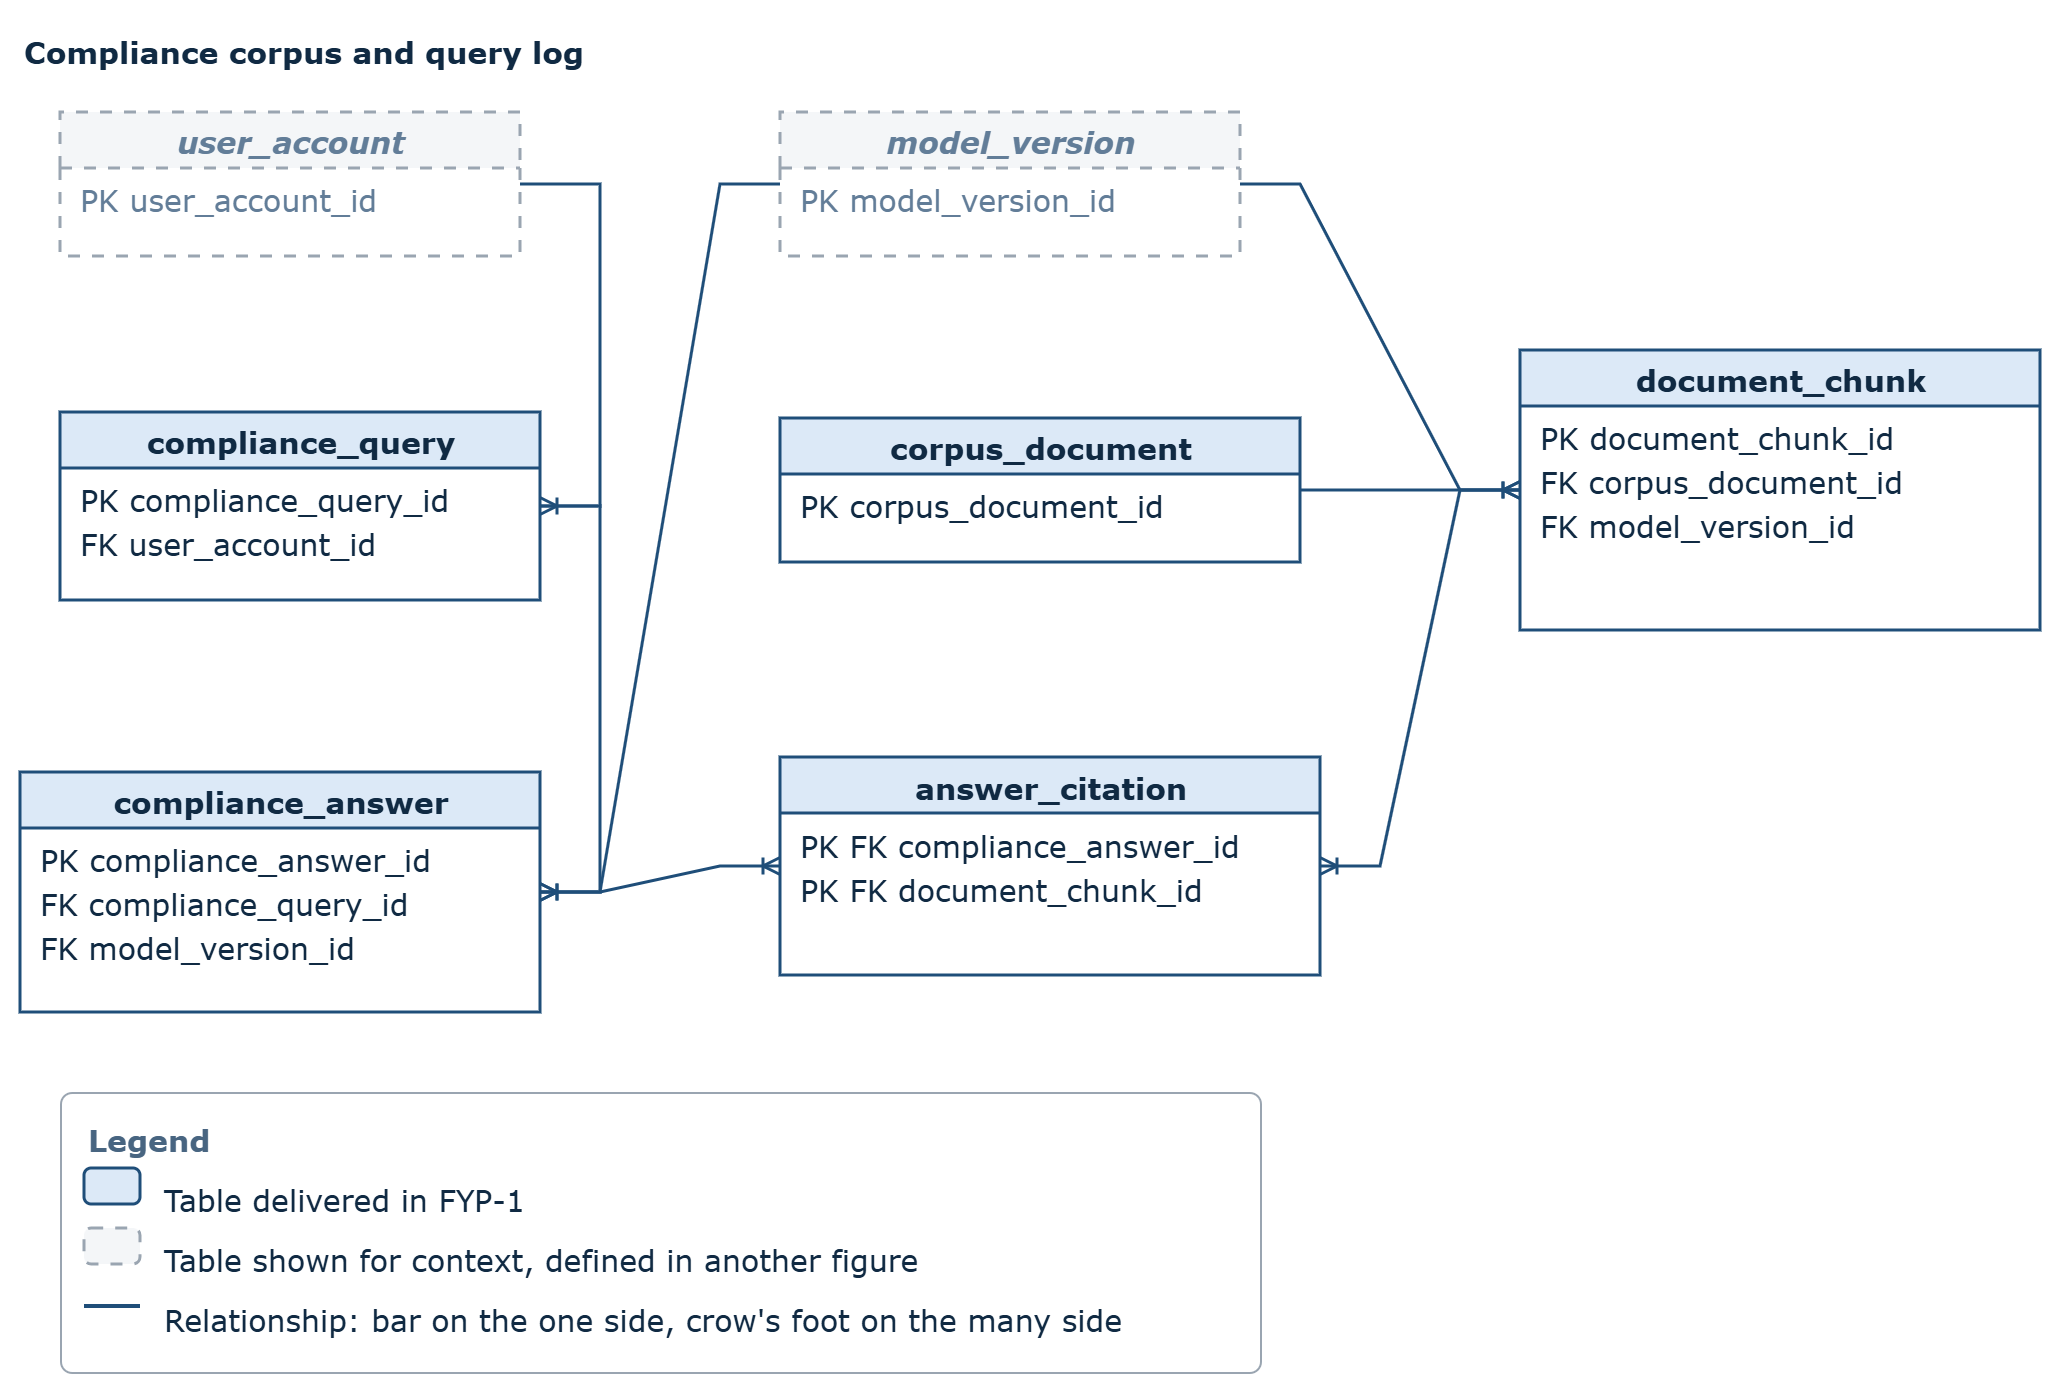
\includegraphics[width=\textwidth,height=0.36\textheight,keepaspectratio]{Figures/fig06_er_compliance}
    \caption{Compliance corpus and query log module}
    \label{fig:er-compliance}
    \capdesc{Compliance source documents and stored answers, with keys.}
\end{figure}

\subsection{Data Dictionary}
The data dictionary lists every attribute of the 41 tables (264 in the current design) with its data type, referenced table, nullability, and meaning. It comes in the next deliverable.

\section{Risk Analysis}
Likelihood is low, medium or high, based on what the team has seen so far. R-15 is unrated because no qualified reviewer has been asked yet.

\subsection{Technical Risks}
\begin{itemize}
    \item R-1 (High): Too few labeled pairs to train the re-ranker. We aim for 150 to 300 and report a pilot against the similarity baseline if we fall short.
    \item R-2 (Medium): The compliance assistant or market synthesis gives an answer its sources do not support. Answers come only from cited passages (NFR-12), or the system abstains (NFR-13).
    \item R-3 (High): The indexed corpus goes out of date. One fee schedule was replaced during the project. Every answer shows its effective date (NFR-14), and we re-check the corpus before the demonstration.
    \item R-4 (Medium): Compliance answers are read as legal or tax advice. The assistant only gives information with sources and dates. Chapter 2 puts legal and tax advice out of scope.
    \item R-5 (Medium): Free tier language model access is rate limited or withdrawn. All calls go through one gateway (NFR-19), so a new provider needs only a configuration change.
    \item R-6 (Medium): LinkedIn OAuth becomes unavailable. The verification score (FR-19) falls back to the other signals, and more profiles go to a reviewer.
    \item R-7 (Medium): Fake profiles pass verification. Detectors fall from about 96\% F1 on manual fakes to about 68\% on language model fakes \cite{ref:gulati2025}. We claim only that rule signals raise the cost of casual fakes. Doubtful profiles go to a reviewer (FR-14, FR-16).
    \item R-8 (Medium): The project reads as an interface over a commercial language model. The re-ranker is the only trained model. The classifiers are offline studies, and every other feature is a prompted module or a rule.
    \item R-9 (High): Roman Urdu has no standard spelling, so a multilingual claim may not hold. We run the benchmark before building on it. FR-9 moves to FYP-2, and FYP-1 is English only.
    \item R-10 (Low): Under deadline pressure, training data is taken from social media or public profiles. This would break PECA 2016 and NFR-9. Our sourcing rule allows only self-registration, consented pilot data, manual writing and synthetic data.
    \item R-11 (Medium): Similarity alone ranks counterparts badly, because investor fit depends on stage, ticket size and thesis. Hard filters come first. FYP-1 adds feature weights, and the FYP-2 re-ranker is tested against them.
    \item R-12 (Low): CVs, pitch content or contact details are exposed. The controls are role based access (NFR-5), contacts hidden until mutual acceptance (NFR-6), file checks (NFR-7), no secrets in the repository (NFR-8) and deletion on request (NFR-10).
    \item R-13 (Medium): Three people cannot finish the build in two semesters. The build order is fixed in Chapter 2, and we drop items from the bottom.
    \item R-14 (Medium): A retrieval pipeline is new to the team. The compliance assistant is first in the build order, so the learning happens early.
\end{itemize}

\subsection{Business Risks}
\begin{itemize}
    \item R-15 (Unassessed): No lawyer or SECP has reviewed the fee design. It takes no equity, runs no transaction and ties no fee to an investment. We claim no compliance until a legal review, which is needed before launch.
    \item R-16 (High): No incubator partnership is secured. The first talk with the LUMS Centre for Entrepreneurship in September 2026 did not become a partnership. We will ask again once the platform is built. Meanwhile we use a student survey, faculty contacts, self-registration and manual writing.
    \item R-17 (Medium): The mentor and investor pools are empty at the demonstration. We seed them with university mentors and the team's connections, and approach investors through incubators.
    \item R-18 (Medium): The panel questions our novelty against existing platforms. Chapter 3 documents a founder and investor matching platform that came first, so we do not claim to be first. We claim four differences: three sides including startup talent, a separate mentor profile, the compliance assistant and multilingual work.
    \item R-19 (Low): Free hosting tiers change terms or end. Services are containerized under one compose file, so a provider change is a redeploy.
\end{itemize}

We rejected two features. A State Bank foreign exchange and offshore corpus carries a different legal risk from registration steps. Gender or location weighting in matching needs its own metrics and ethical review first.

\section{Conclusion}
This chapter specified The Founder's Carnet through 17 features and 31 functional requirements. Twenty-five are built in FYP-1, four move to FYP-2, and two are split between the two semesters. The 23 non-functional requirements make quality measurable. Ten use cases cover the main behavior, including the assistant declining to answer. Two items are still open. No qualified reviewer has checked the fee model, so R-15 has no rating and we claim no compliance. The labeled dataset for matching does not exist yet, and R-1 says what we report if it never does. Chapter 5 turns this specification into a design.

\chapter{High-Level and Low-Level Design}
Chapter 4 said what the platform must do. This chapter shows how we build it. Two decisions shape the design. The matching re-ranker is the only trained model, and the three classifiers in Section~\ref{sec:classifiers} are offline studies. Every other intelligent feature is a prompted language model call. The work also runs across two semesters (Section~\ref{sec:fallback}), so some parts are designed now for FYP-2.

\section{System Overview}
The Founder's Carnet is a web platform for founders, startup job seekers, mentors and investors in Pakistan. Administrators verify and moderate profiles. The Next.js client talks only to a FastAPI gateway, which checks the login, role and request format first. Behind the gateway are six services: startup intelligence, compliance retrieval, matching and ranking, authentication, profiles, and administration. They share one PostgreSQL database with pgvector. Redis and Celery run slow jobs like embedding generation. Every model call goes through one LLM gateway to Gemini. Firecrawl and Playwright collect public sources. Each feature follows one path. The input becomes a structured schema, and a prompted template or a ranking step reasons over it. The result is checked against evidence and cited where it matters. If the evidence is missing, the system says it cannot answer.

\begin{figure}[H]
\centering
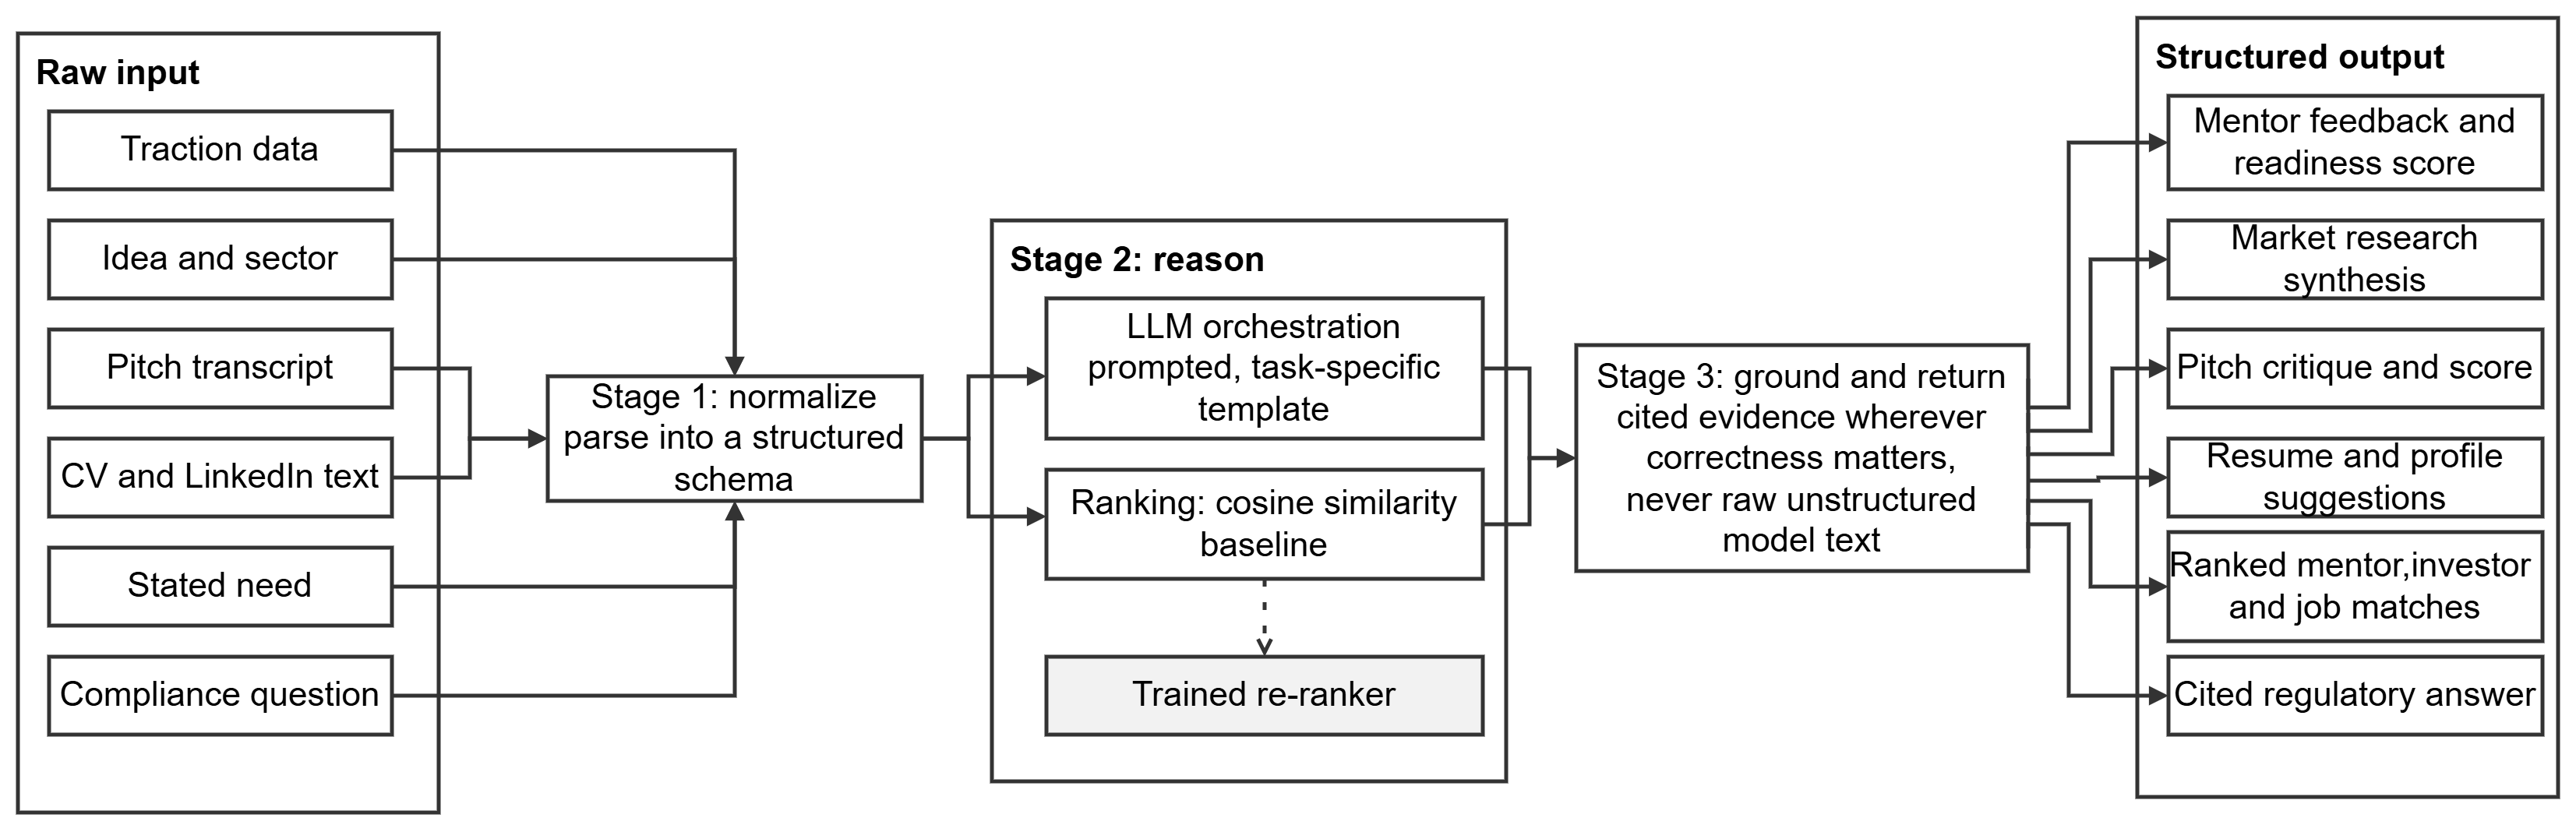
\includegraphics[width=\textwidth,height=0.42\textheight,keepaspectratio]{Figures/fig13_core_ai_engine.png}
\caption{Core AI reasoning engine: normalize, reason, ground}
\label{fig:core-engine}
\capdesc{Six kinds of raw input pass through three stages into six kinds of structured output.}
\end{figure}

\section{Design Considerations}

\subsection{Assumptions and Dependencies}
We treat every outside service as swappable. Higher Gemini models were unreliable under free-tier load, so we use the Google AI Studio free tier with Gemini 2.5 or lower. Its rate limit gives the five concurrent requests in NFR-2, and all calls go through one gateway (NFR-19). LinkedIn OAuth is the strongest signal for mentors and investors (FR-12), but a student application may not get API access. Without it, the score (FR-19) uses the other signals and more profiles go to a reviewer. We expect four changes later: the trained re-ranker, Urdu and Roman Urdu (FR-9), a bigger compliance corpus, and a new model provider. Each one replaces a single part behind a boundary that already exists.

\subsection{General Constraints}
Free tiers set the size. We target 50 concurrent users (NFR-1) and five concurrent model requests, and extra requests wait in a queue. We do not need a local GPU, because embeddings run in background jobs. The legal limits in Chapter 2 also apply: no equity, no transactions and no legal advice.

\subsection{Goals and Development Methods}
We start with the simplest thing we can evaluate, so every part can be explained in a defense and measured against a baseline. Where correctness matters, the system returns its evidence with the answer or nothing at all. The re-ranker is the only trained model, and each replaceable part has its own boundary. Sprints follow the delivery priority in Section~\ref{sec:fallback}: foundations, the compliance assistant, matching, then the other prompted modules. We rejected Waterfall because some answers only appear after something is built, like the chunking strategy for the regulatory corpus. The Rational Unified Process was too heavy for three developers. Decisions go into a dated log. Every pull request runs linting and tests through GitHub Actions (NFR-23) and needs approval from someone other than the last pusher. Schema changes are versioned migrations (NFR-22).

\Needspace{30\baselineskip}
\section{System Architecture}
Figure~\ref{fig:architecture} shows a client, one API gateway, six services, a shared database and a background queue. A request goes from the client through the gateway to one service, which reads and writes the database. Matching never calls a language model. Every prompted feature reaches Gemini only through the LLM gateway, and slow work runs in the background through Redis and Celery. Section~\ref{sec:strategies} explains why the services are split by responsibility but deployed together.

\begin{figure}[H]
\centering
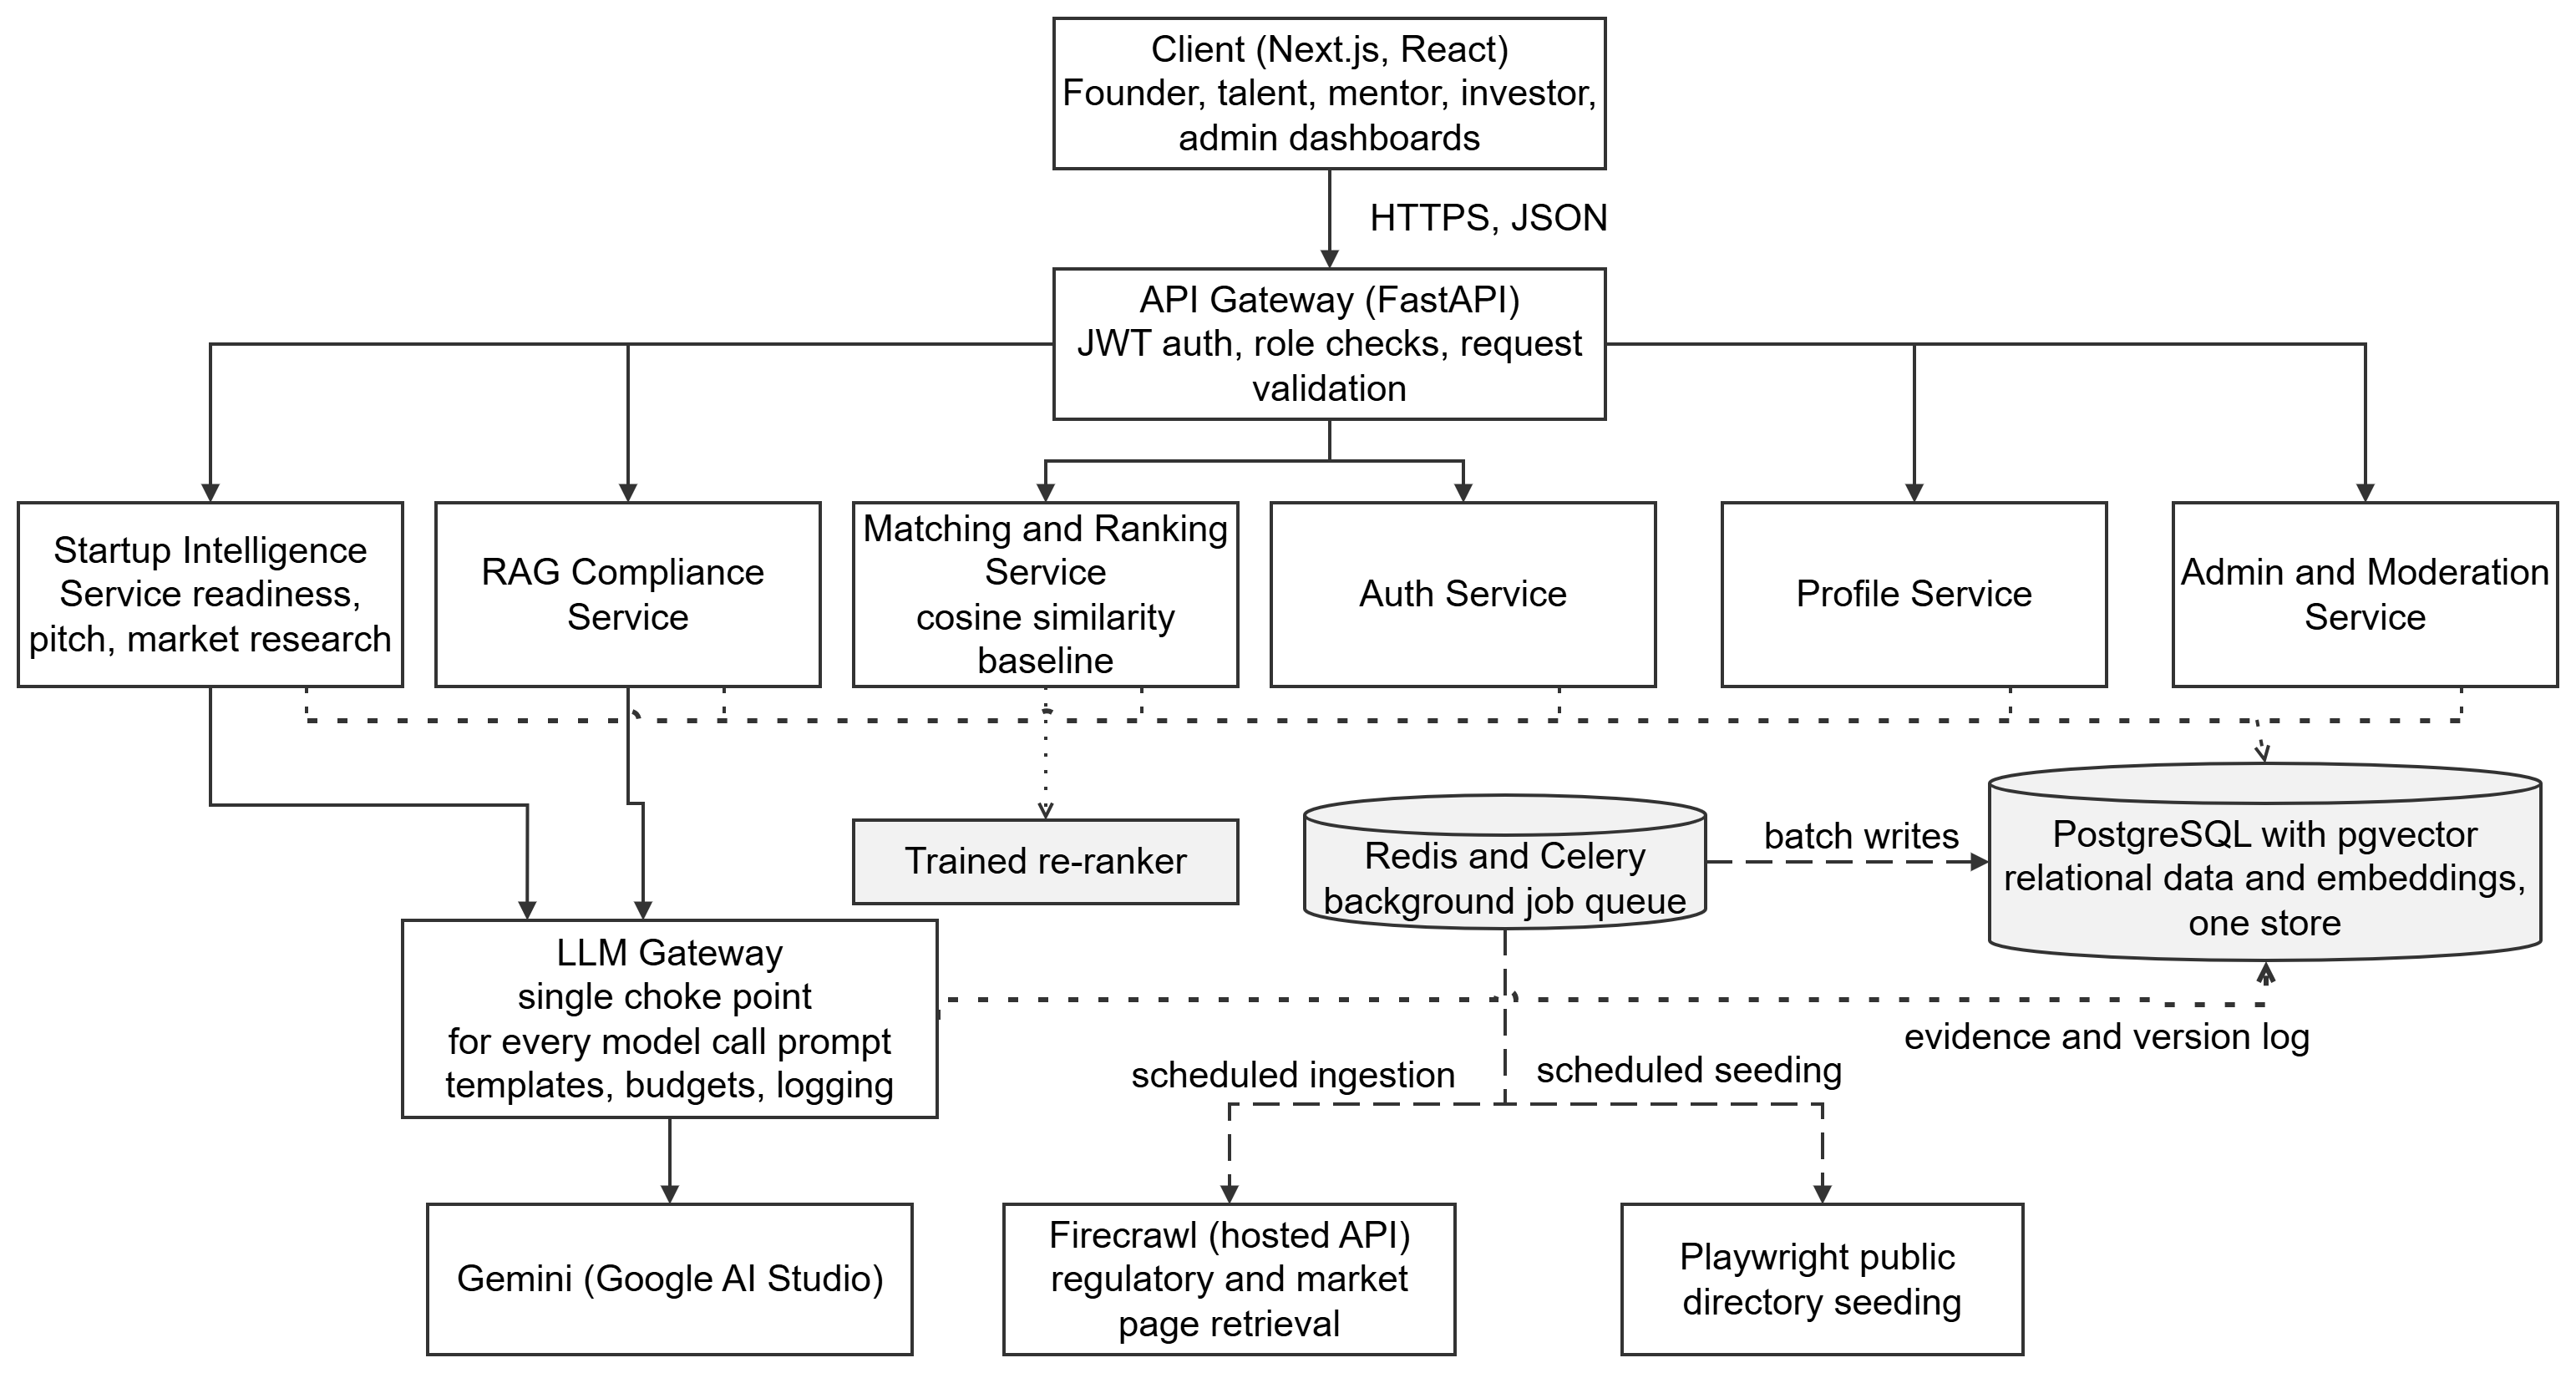
\includegraphics[width=\textwidth,height=0.42\textheight,keepaspectratio]{Figures/fig14_architecture_highlevel.png}
\caption{High-level system architecture}
\label{fig:architecture}
\capdesc{The client reaches six services through the API gateway. Model calls pass through the LLM gateway.}
\end{figure}


\Needspace{22\baselineskip}
\subsection{Subsystem Architecture}
Four parts need more detail: matching, compliance retrieval, profile verification, and background pipeline.

\Needspace{22\baselineskip}
\subsubsection{Matching and Ranking}
Matching runs in two stages (Figure~\ref{fig:matching}). Stage 1 pulls the top-K candidates by pgvector cosine similarity and filters them by sector, stage and geography. Stage 2 ranks what is left. In FYP-1 it scores five factors (sector, stage, skills, availability and ticket fit) and ranks by cosine score and factor weights. In FYP-2 a trained re-ranker takes over, once we collect a human relevance dataset. We test it against the cosine baseline with NDCG@K and MRR. Contact details appear only after both sides accept.

\begin{figure}[H]
\centering
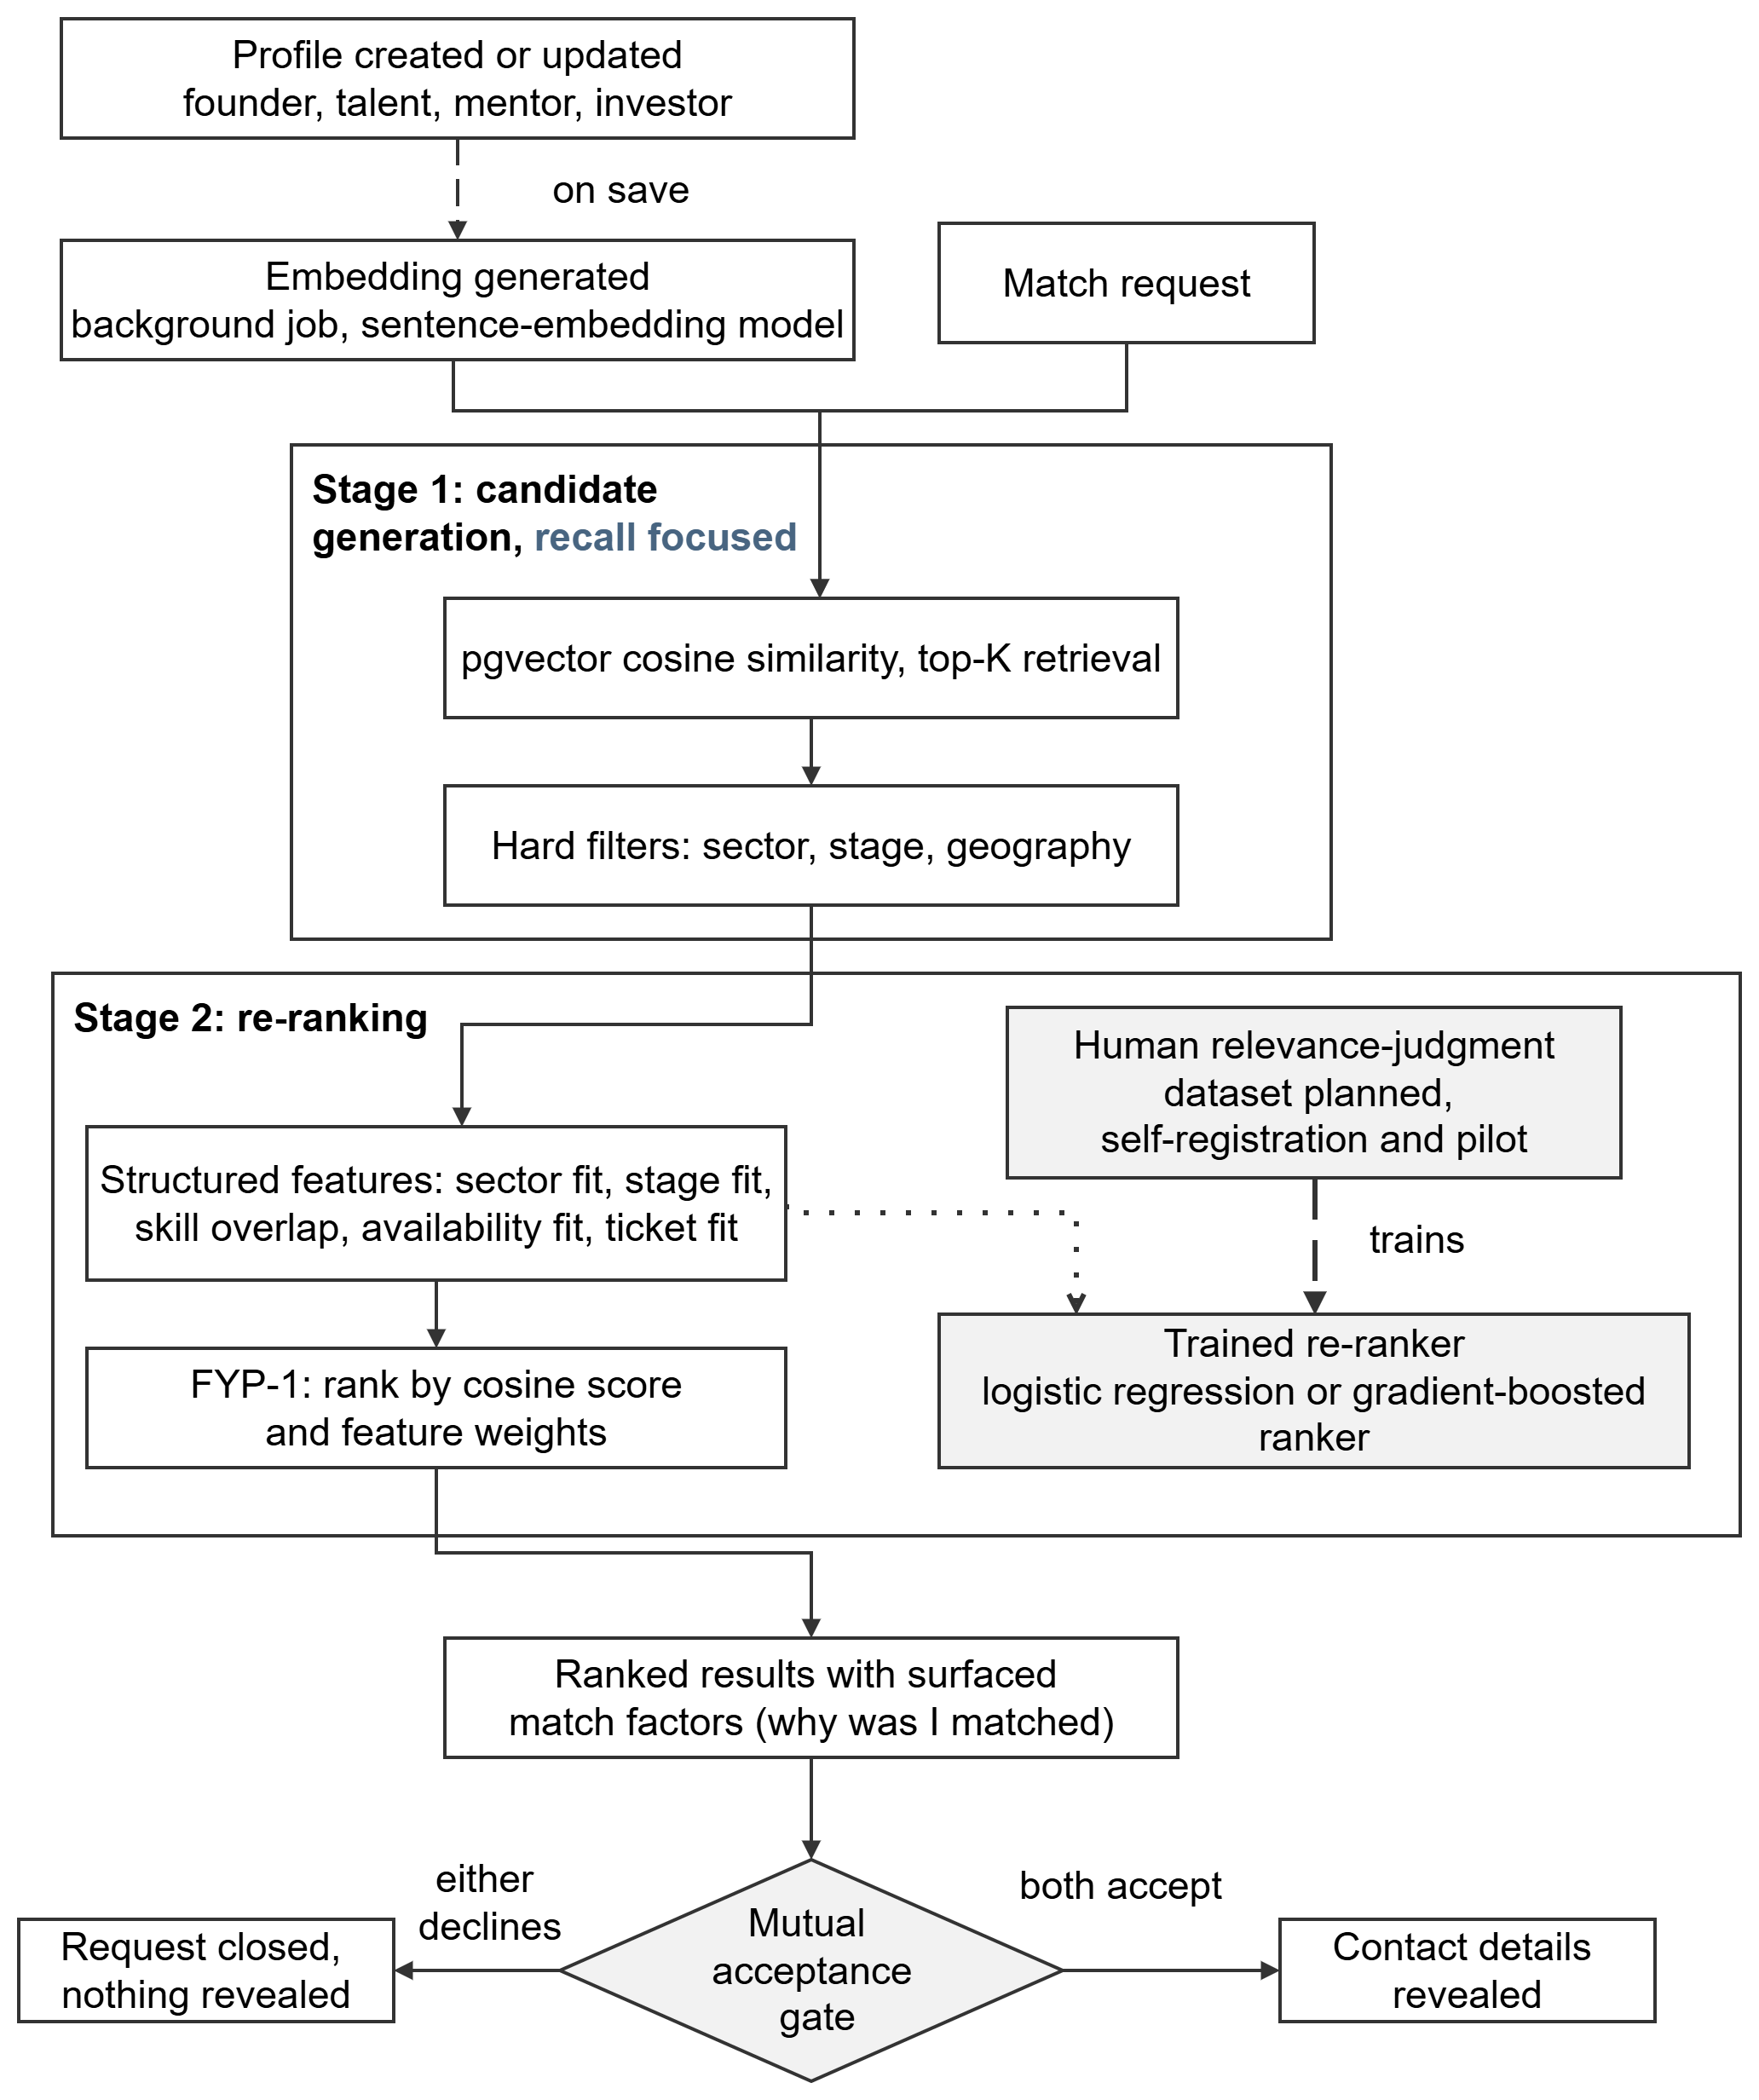
\includegraphics[width=\textwidth,height=0.42\textheight,keepaspectratio]{Figures/fig15_matching_subsystem.png}
\caption{Matching and ranking subsystem with mutual acceptance gate}
\label{fig:matching}
\capdesc{Candidates are retrieved and filtered, ranked by similarity and factor weights in FYP-1.}
\end{figure}

\Needspace{22\baselineskip}
\subsubsection{Retrieval and Compliance}
The assistant embeds the question and retrieves the top passages from the corpus in PostgreSQL (Figure~\ref{fig:compliance}). It declines if no passage supports an answer, if validation fails, or if the question asks for case-specific advice. Every query is logged with its outcome, and a decline also logs its reason. FYP-1 answers in English only, and Urdu and Roman Urdu come in FYP-2.

\begin{figure}[H]
\centering
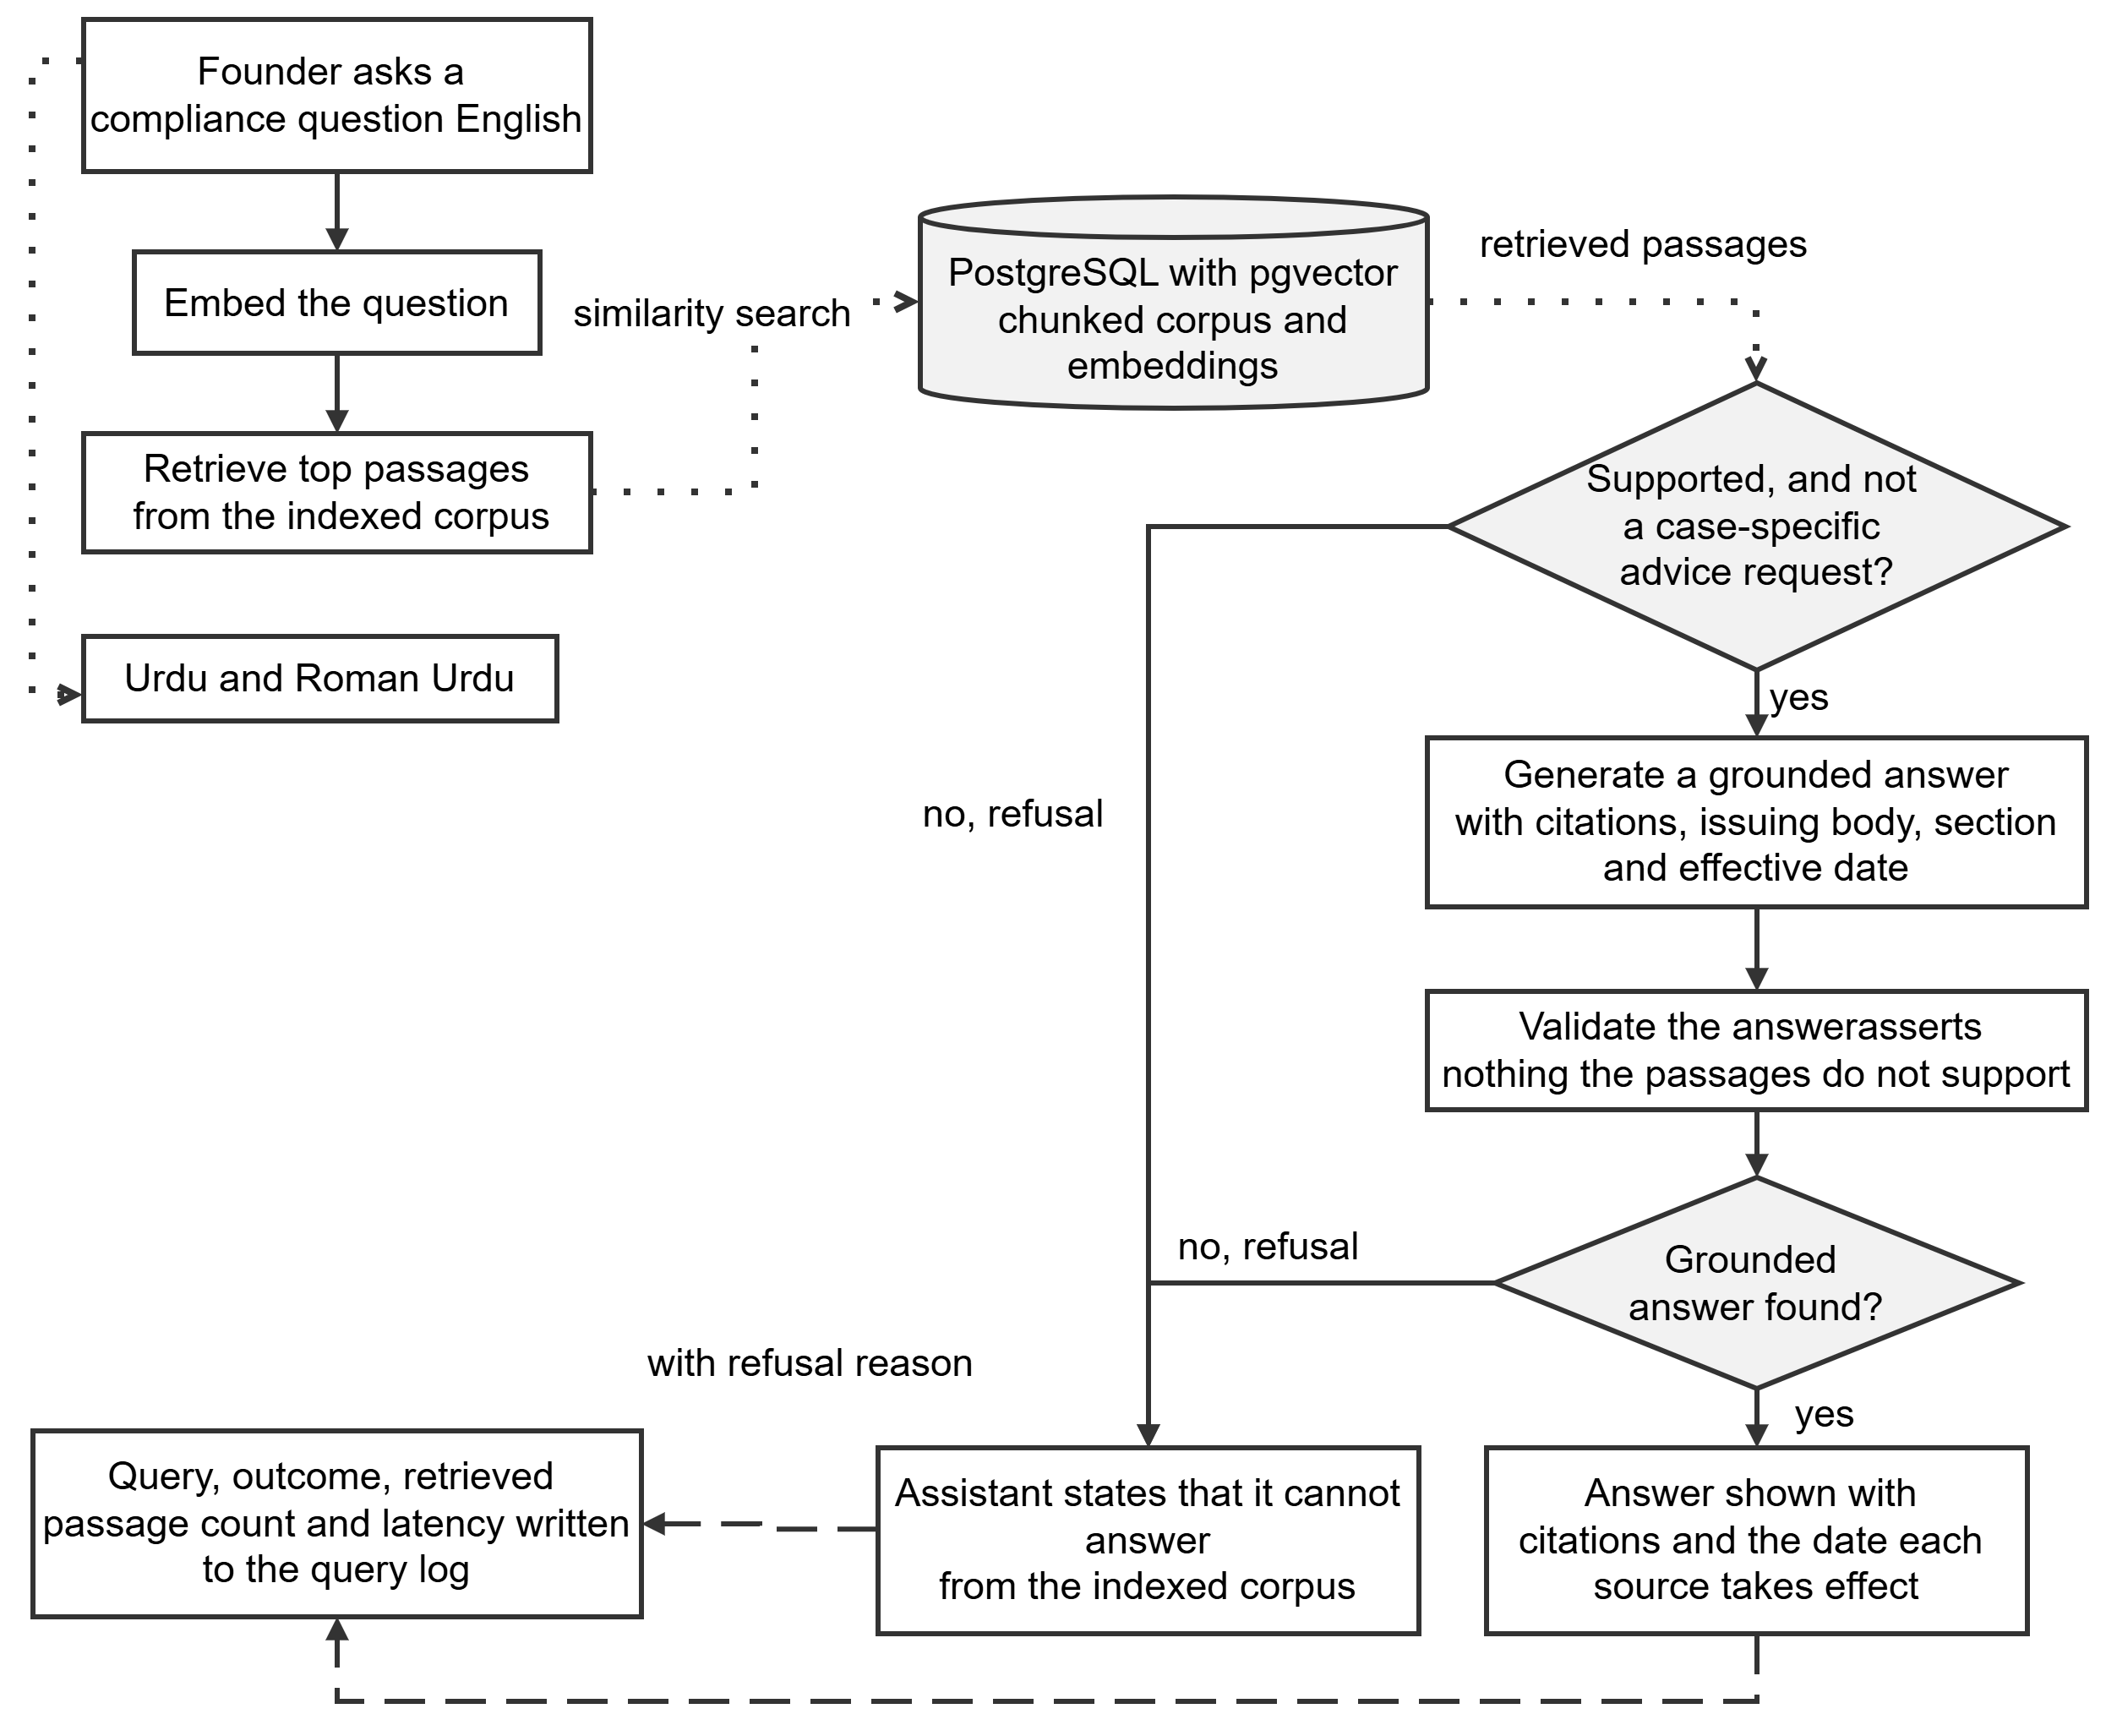
\includegraphics[width=\textwidth,height=0.42\textheight,keepaspectratio]{Figures/fig16_arch_compliance.png}
\caption{Compliance question flow with abstention path}
\label{fig:compliance}
\capdesc{The assistant can abstain after retrieval or after validation, and every query is logged.}
\end{figure}

\Needspace{22\baselineskip}
\subsubsection{Profile Verification}
A submitted profile gets an automated score from five signals: LinkedIn OAuth, an SECP check, profile completeness, GitHub activity for talent, and portfolio link consistency (Figure~\ref{fig:verification}). Only the link check is a prompted call, and the other four are rules we wrote. A reviewer decides middle scores and appeals, and a rejection after appeal is final. Every decision is logged with its reason, signals and threshold version.

\begin{figure}[H]
\centering
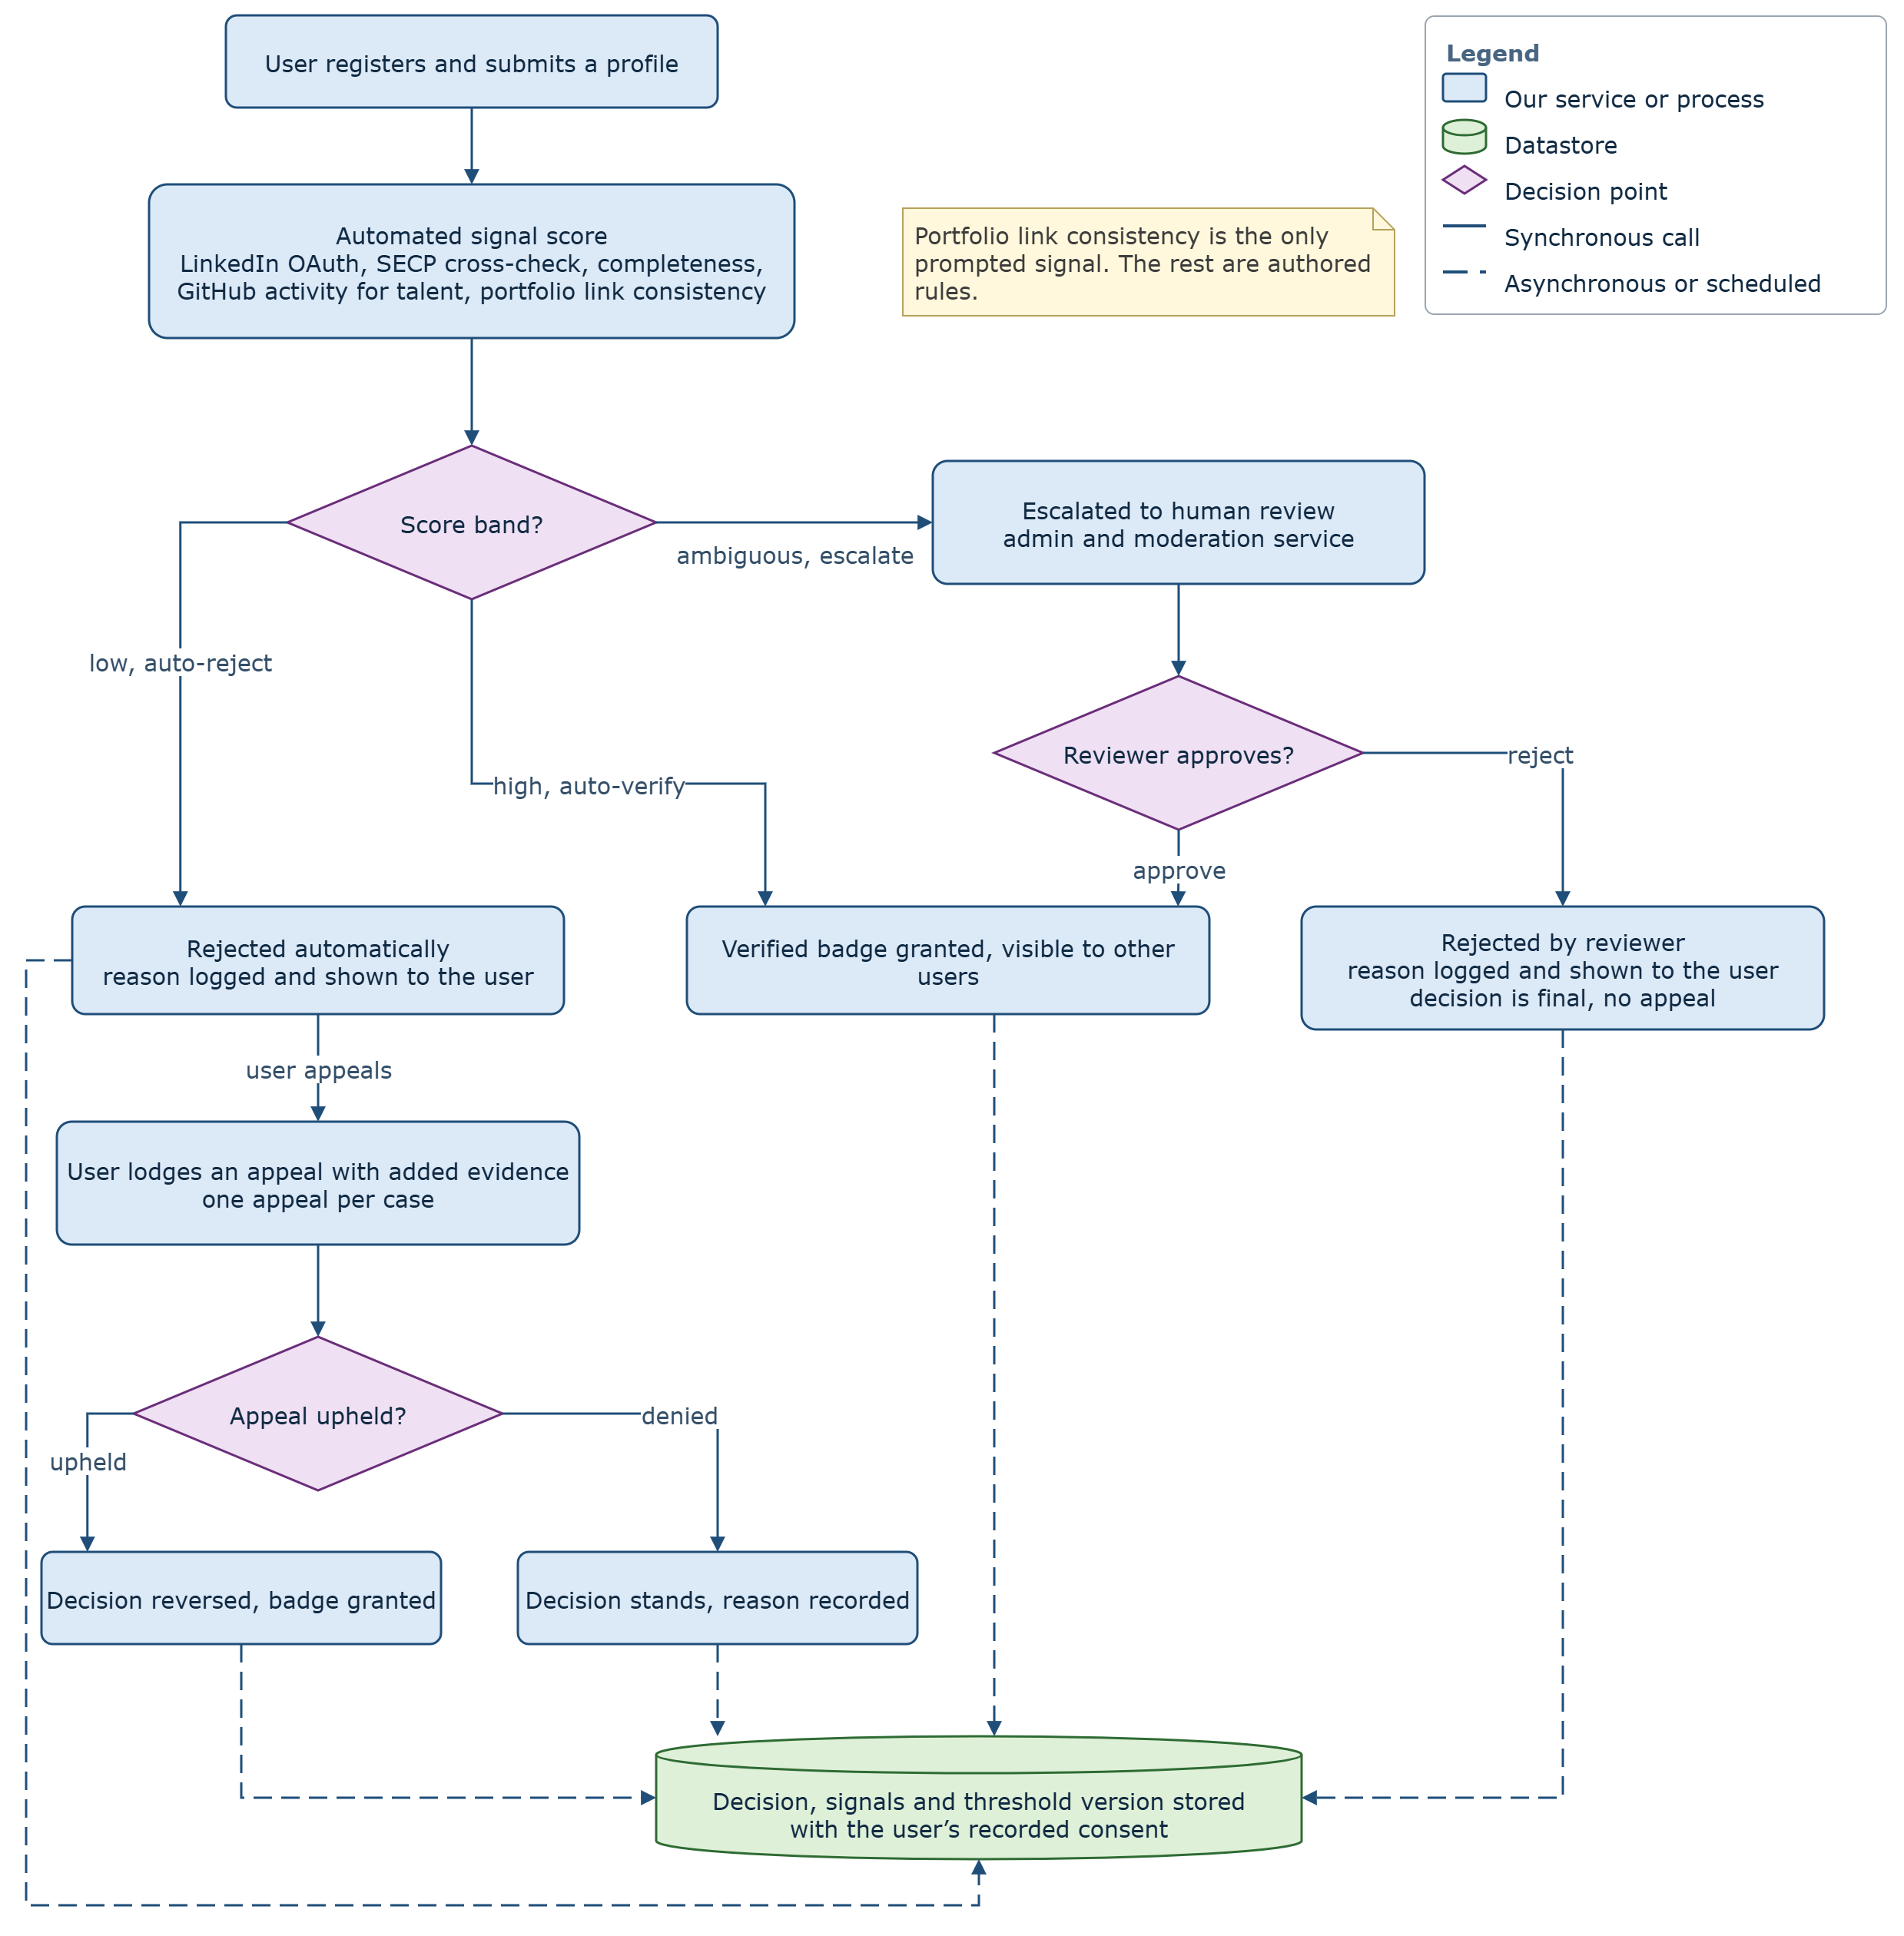
\includegraphics[width=0.7\textwidth]{Figures/fig17_arch_verification.png}
\caption{Profile verification with three score bands and appeal path}
\label{fig:verification}
\capdesc{Scores route to auto-verify, human review or auto-reject, and only automatic rejection can be appealed.}
\end{figure}

\Needspace{22\baselineskip}
\subsubsection{Background Pipeline}
Celery and cron run the background jobs, which write to PostgreSQL (Figure~\ref{fig:background}). Ingestion pulls whitelisted SECP, FBR and PSEB pages through Firecrawl, then chunks, embeds and indexes them. Playwright seeds the directory from public accelerator and incubator pages. Embeddings are regenerated when a profile is edited or the embedding model changes. In FYP-2 a batch job trains the re-ranker, and a new version goes live only if it does not regress against the cosine baseline.

\begin{figure}[H]
\centering
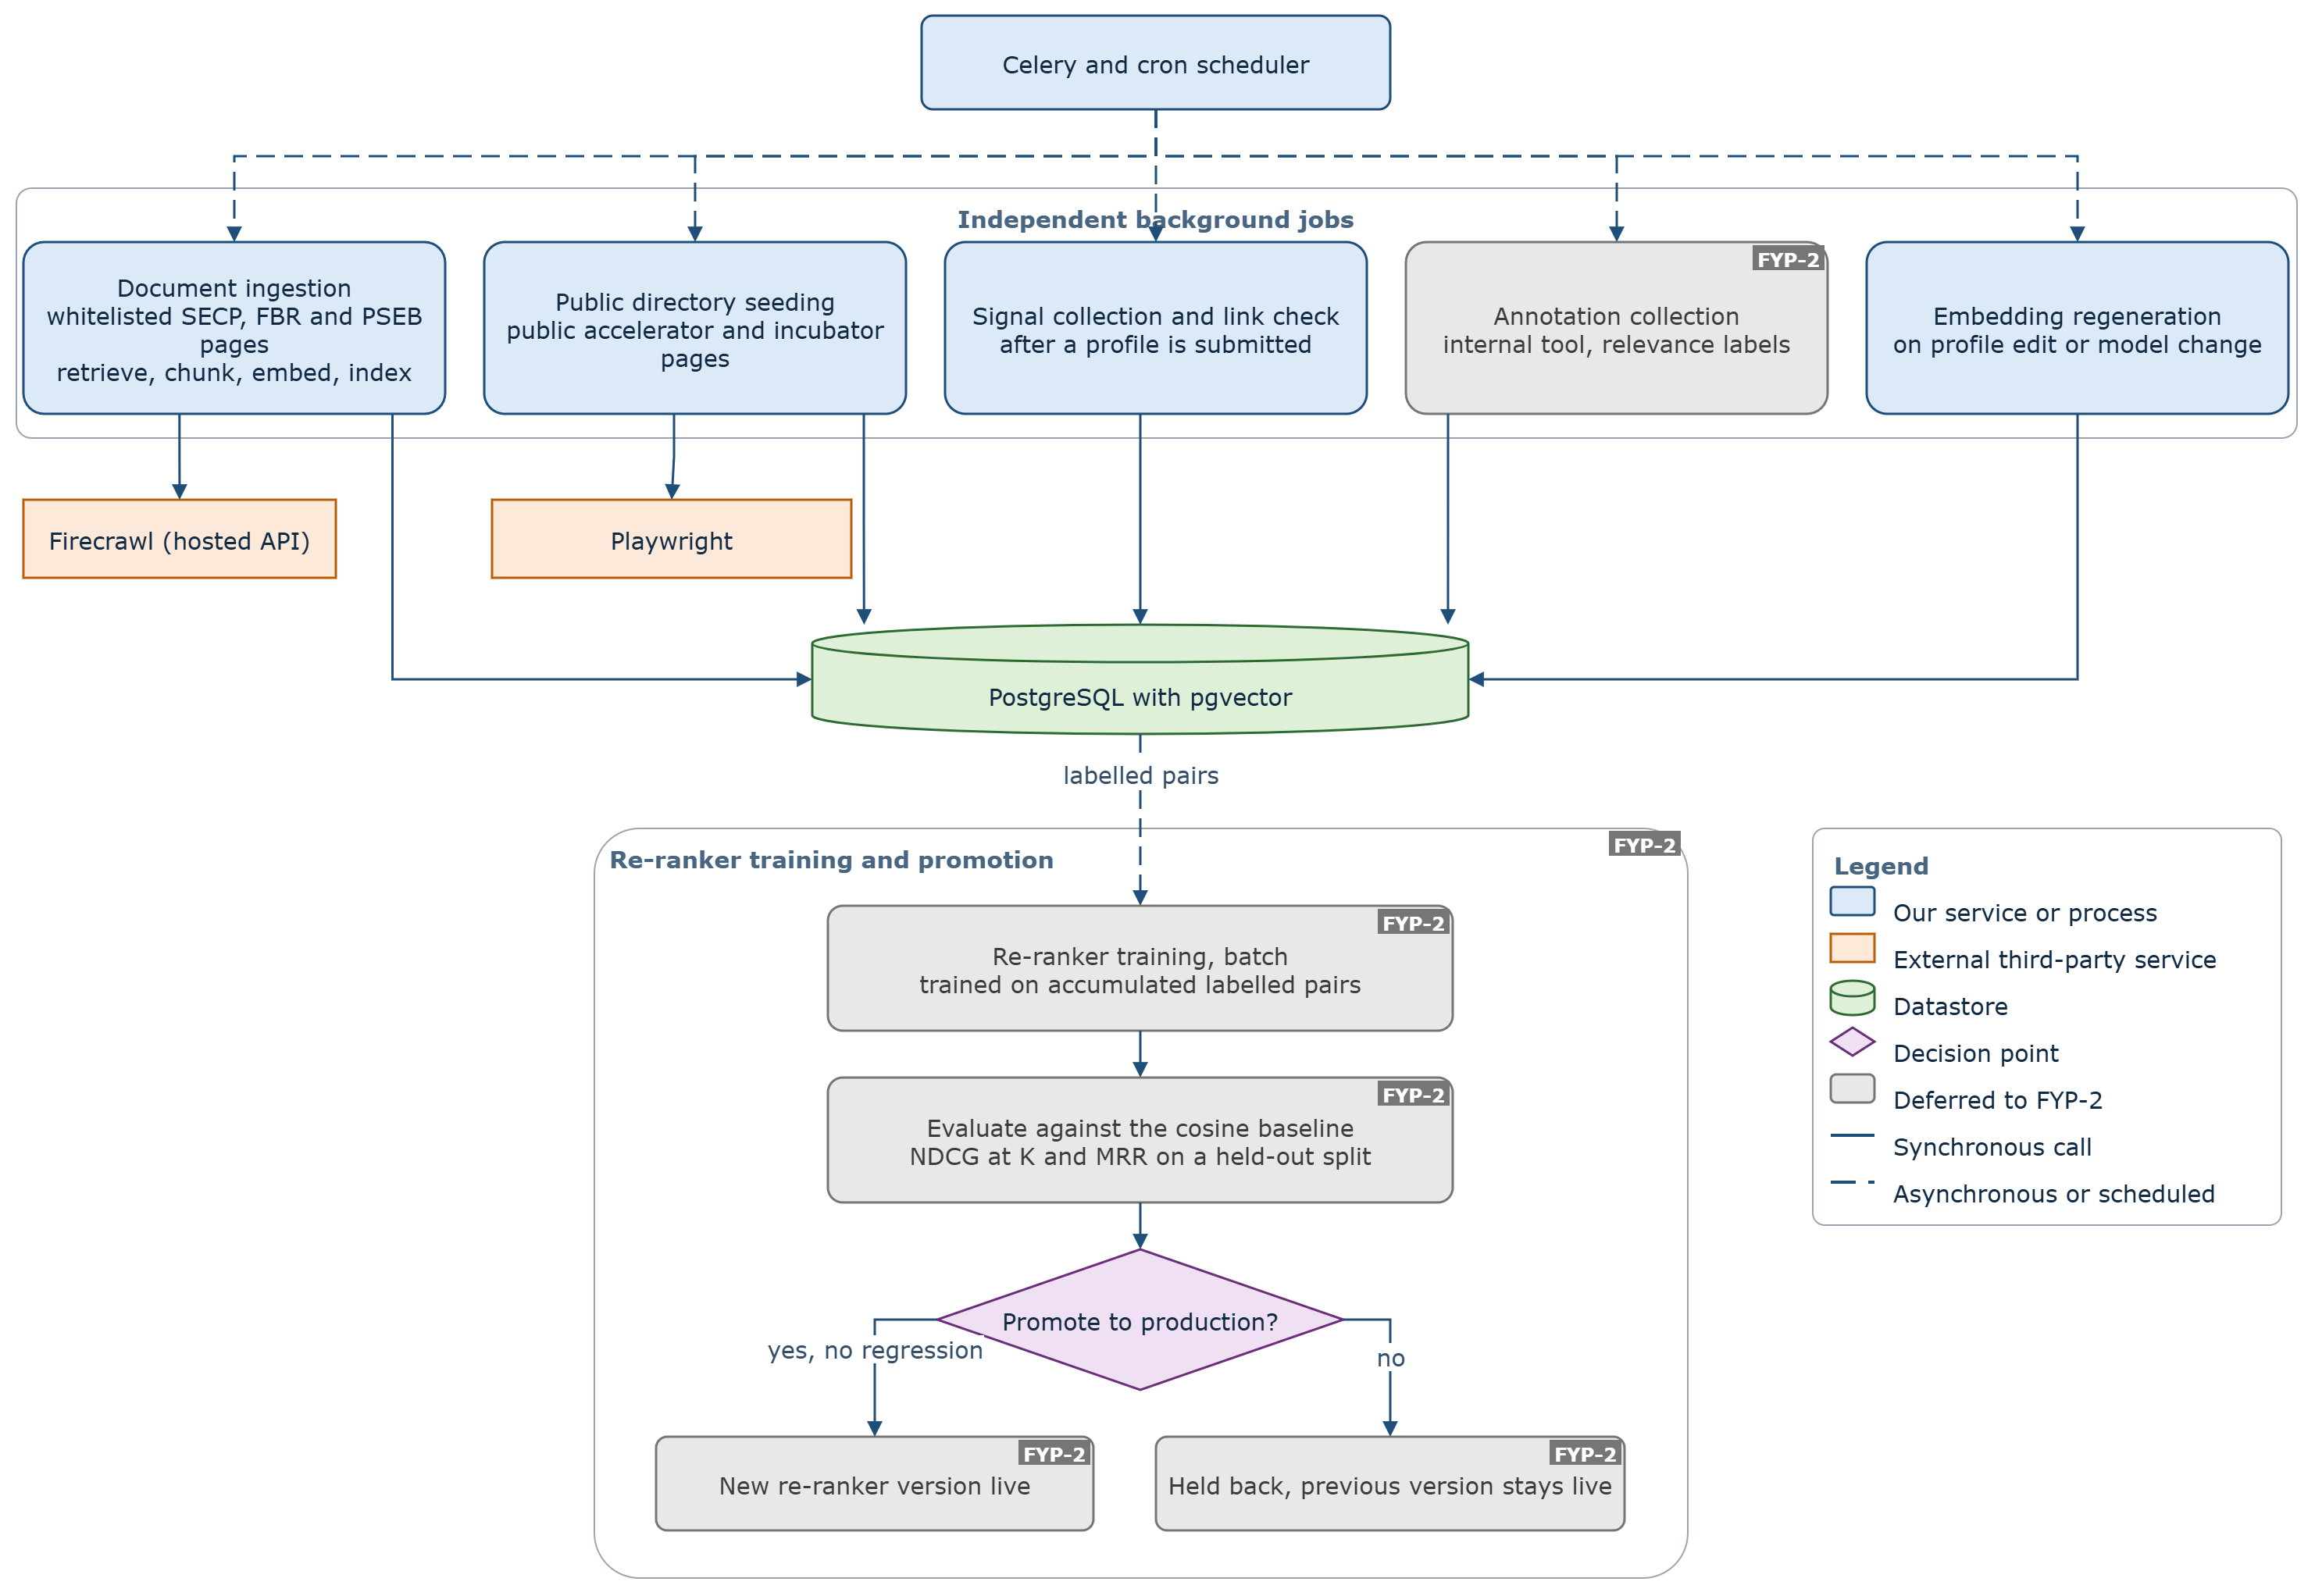
\includegraphics[width=\textwidth,height=0.42\textheight,keepaspectratio]{Figures/fig18_arch_background.png}
\caption{Background jobs and the FYP-2 training loop}
\label{fig:background}
\capdesc{Five background jobs write to the database, and a training loop with a release check is added in FYP-2.}
\end{figure}

\section{Architectural Strategies}
\label{sec:strategies}

\subsection{A Single Gateway for Every Language Model Call}
Every language model call goes through one internal gateway. It holds the prompt templates, enforces the concurrency limit (NFR-2) and logs what was sent and returned. No feature calls a provider directly. Changing provider is then one edit, and a stored assessment can state which prompt version it used.

\subsection{Relational Records and Vectors in One Store}
PostgreSQL with pgvector holds profiles, corpus records and their embeddings together (NFR-20). We ruled out a separate vector database because it adds a second store to keep consistent and probably a paid tier. At our scale pgvector is enough. A match query can also filter on columns and search vectors in one step.

\subsection{Two-Stage Matching}
Matching first picks candidates by cosine similarity with hard filters. Then it re-ranks a short list on structured features. A cross-encoder was too costly, and with only 150 to 300 labeled pairs it would likely overfit. The split also fits the two semesters: FYP-1 ranks by similarity and feature weights, and FYP-2 adds the trained re-ranker.

\subsection{Grounded Generation with Abstention}
The compliance assistant answers only from retrieved passages and attaches the source and effective date. When nothing supports an answer, it says so. We did not fine-tune on the corpus, because the corpus keeps changing and a fine-tuned model cannot cite a passage. Answering without retrieval was also out, since commercial legal research tools hallucinated 17 to 33\% of the time \cite{ref:magesh2025}.

\subsection{Services Separated by Responsibility, Deployed Together}
The backend is split into services in the code but runs as a few container instances. Full microservices were too much work for three developers, and free hosting tiers cannot run one instance per service. We kept matching and retrieval separate because they are the two parts most likely to be pulled out later.

\subsection{Deferred Work Through a Queue}
Embedding, ingestion, directory seeding, link checks and (in FYP-2) re-ranker training run as Celery and Redis background jobs. Embedding a document set takes longer than any acceptable response time. A failing link check should also not fail the profile submission that triggered it.

\subsection{Visible Degradation}
Where a component can fail, the user sees what happened. At the concurrency limit, the request is queued and shown as queued. If a model call fails, the previous readiness assessment stays and the user can retry. If a verification signal is missing, the score uses the remaining signals and more profiles go to human review.

\Needspace{30\baselineskip}
\section{Domain Model/Class Diagram}
\label{sec:domain}

\Needspace{22\baselineskip}
\subsection{Class Diagram}
Figure~\ref{fig:class-diagram} shows the 23 core classes of the platform in five modules. It is a domain model, so it shows only main attributes and multiplicities. The entity-relationship figures in Chapter 4 show all 41 tables. The user account is the hub. It has at most one founder, talent, mentor or investor profile, and a founder profile registers any number of startups. Consent records, verification signals, dimension scores, match results, match factors and document chunks cannot exist without their owner.

\begin{figure}[H]
\centering
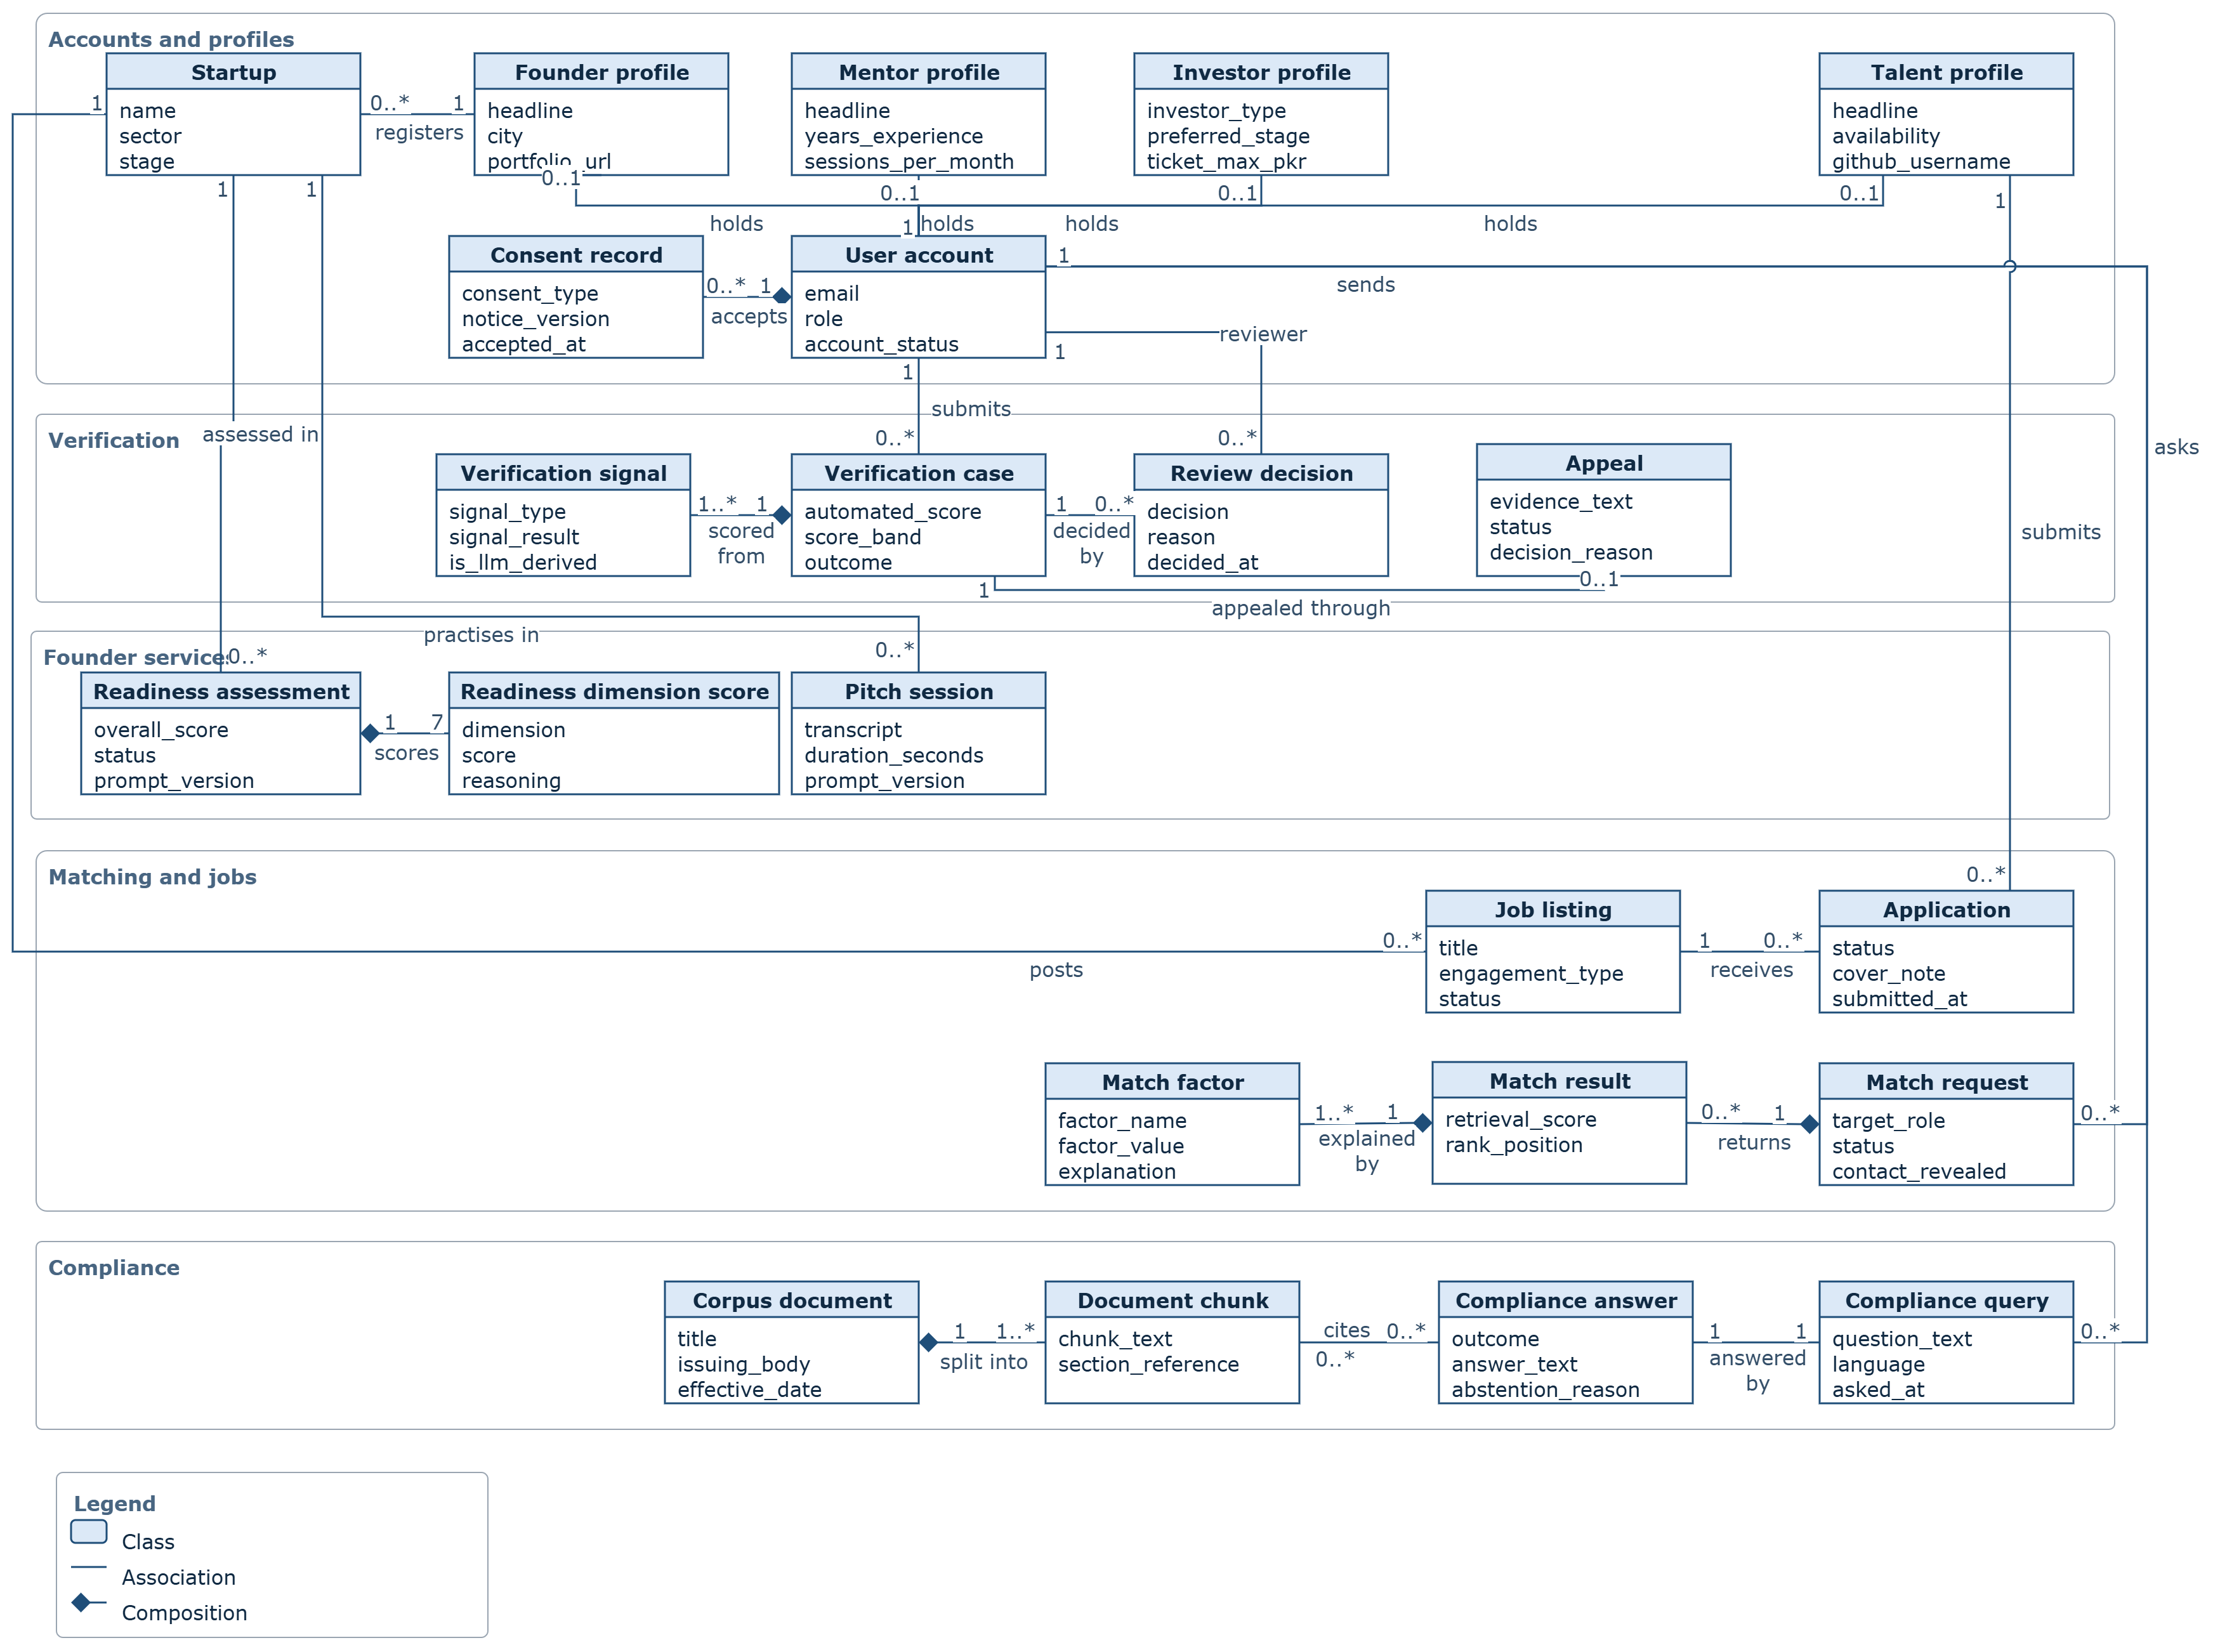
\includegraphics[width=\textwidth,height=0.42\textheight,keepaspectratio]{Figures/fig19_class_domain_model.png}
\caption{Domain model of The Founder's Carnet}
\label{fig:class-diagram}
\capdesc{The 23 classes of the platform's core data in five modules, with the multiplicity of each relationship.}
\end{figure}

\subsection{Sequence Diagrams}
Four sequence diagrams show the order of calls in the main flows. They leave out the client and the API gateway, which applies JWT authentication and role checks before any request reaches a service.

\Needspace{22\baselineskip}
\subsubsection{Registration}
Figure~\ref{fig:seq-register} shows registration by email and by LinkedIn. No account is created unless the notice is accepted.

\begin{figure}[H]
\centering
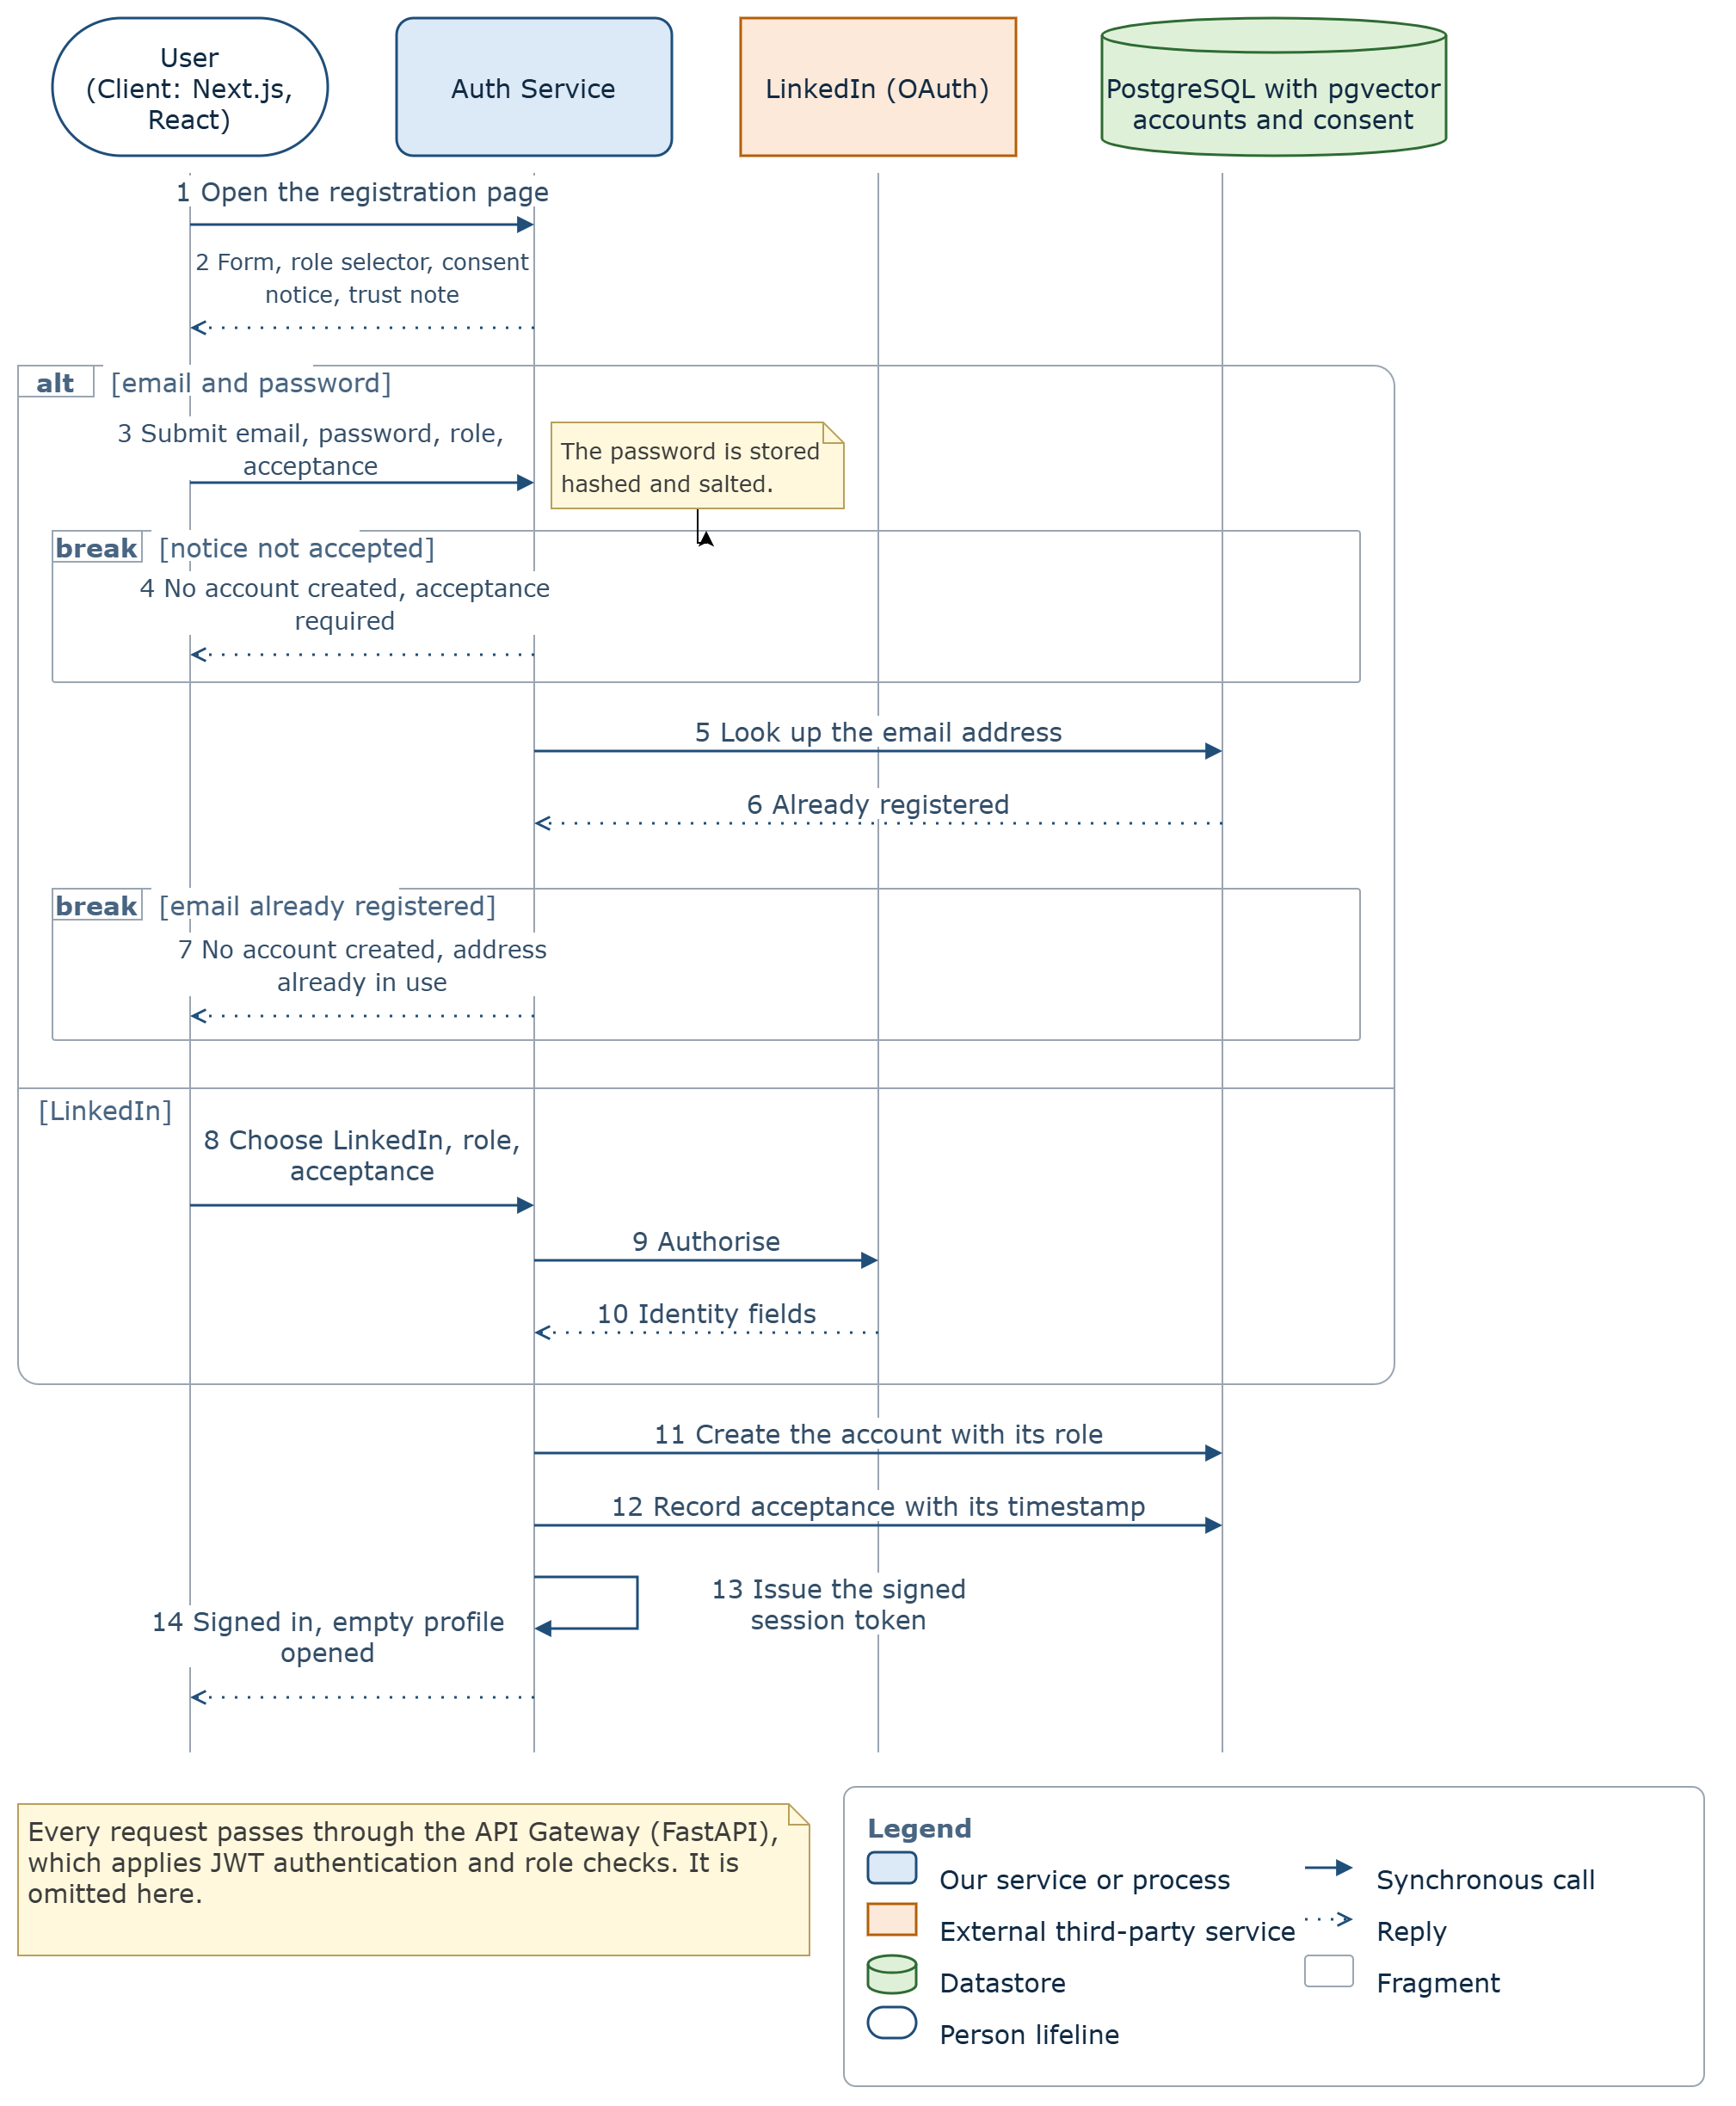
\includegraphics[height=0.6\textheight,keepaspectratio]{Figures/fig20_seq_register.png}
\caption{Registration with consent acceptance}
\label{fig:seq-register}
\capdesc{A user registers by email or LinkedIn, and no account is created unless the consent notice is accepted.}
\end{figure}

\Needspace{22\baselineskip}
\subsubsection{Verification, Review and Appeal}

Figure~\ref{fig:seq-verification} shows verification from submission to the final decision. A second appeal is declined as final.

\begin{figure}[H]
\centering
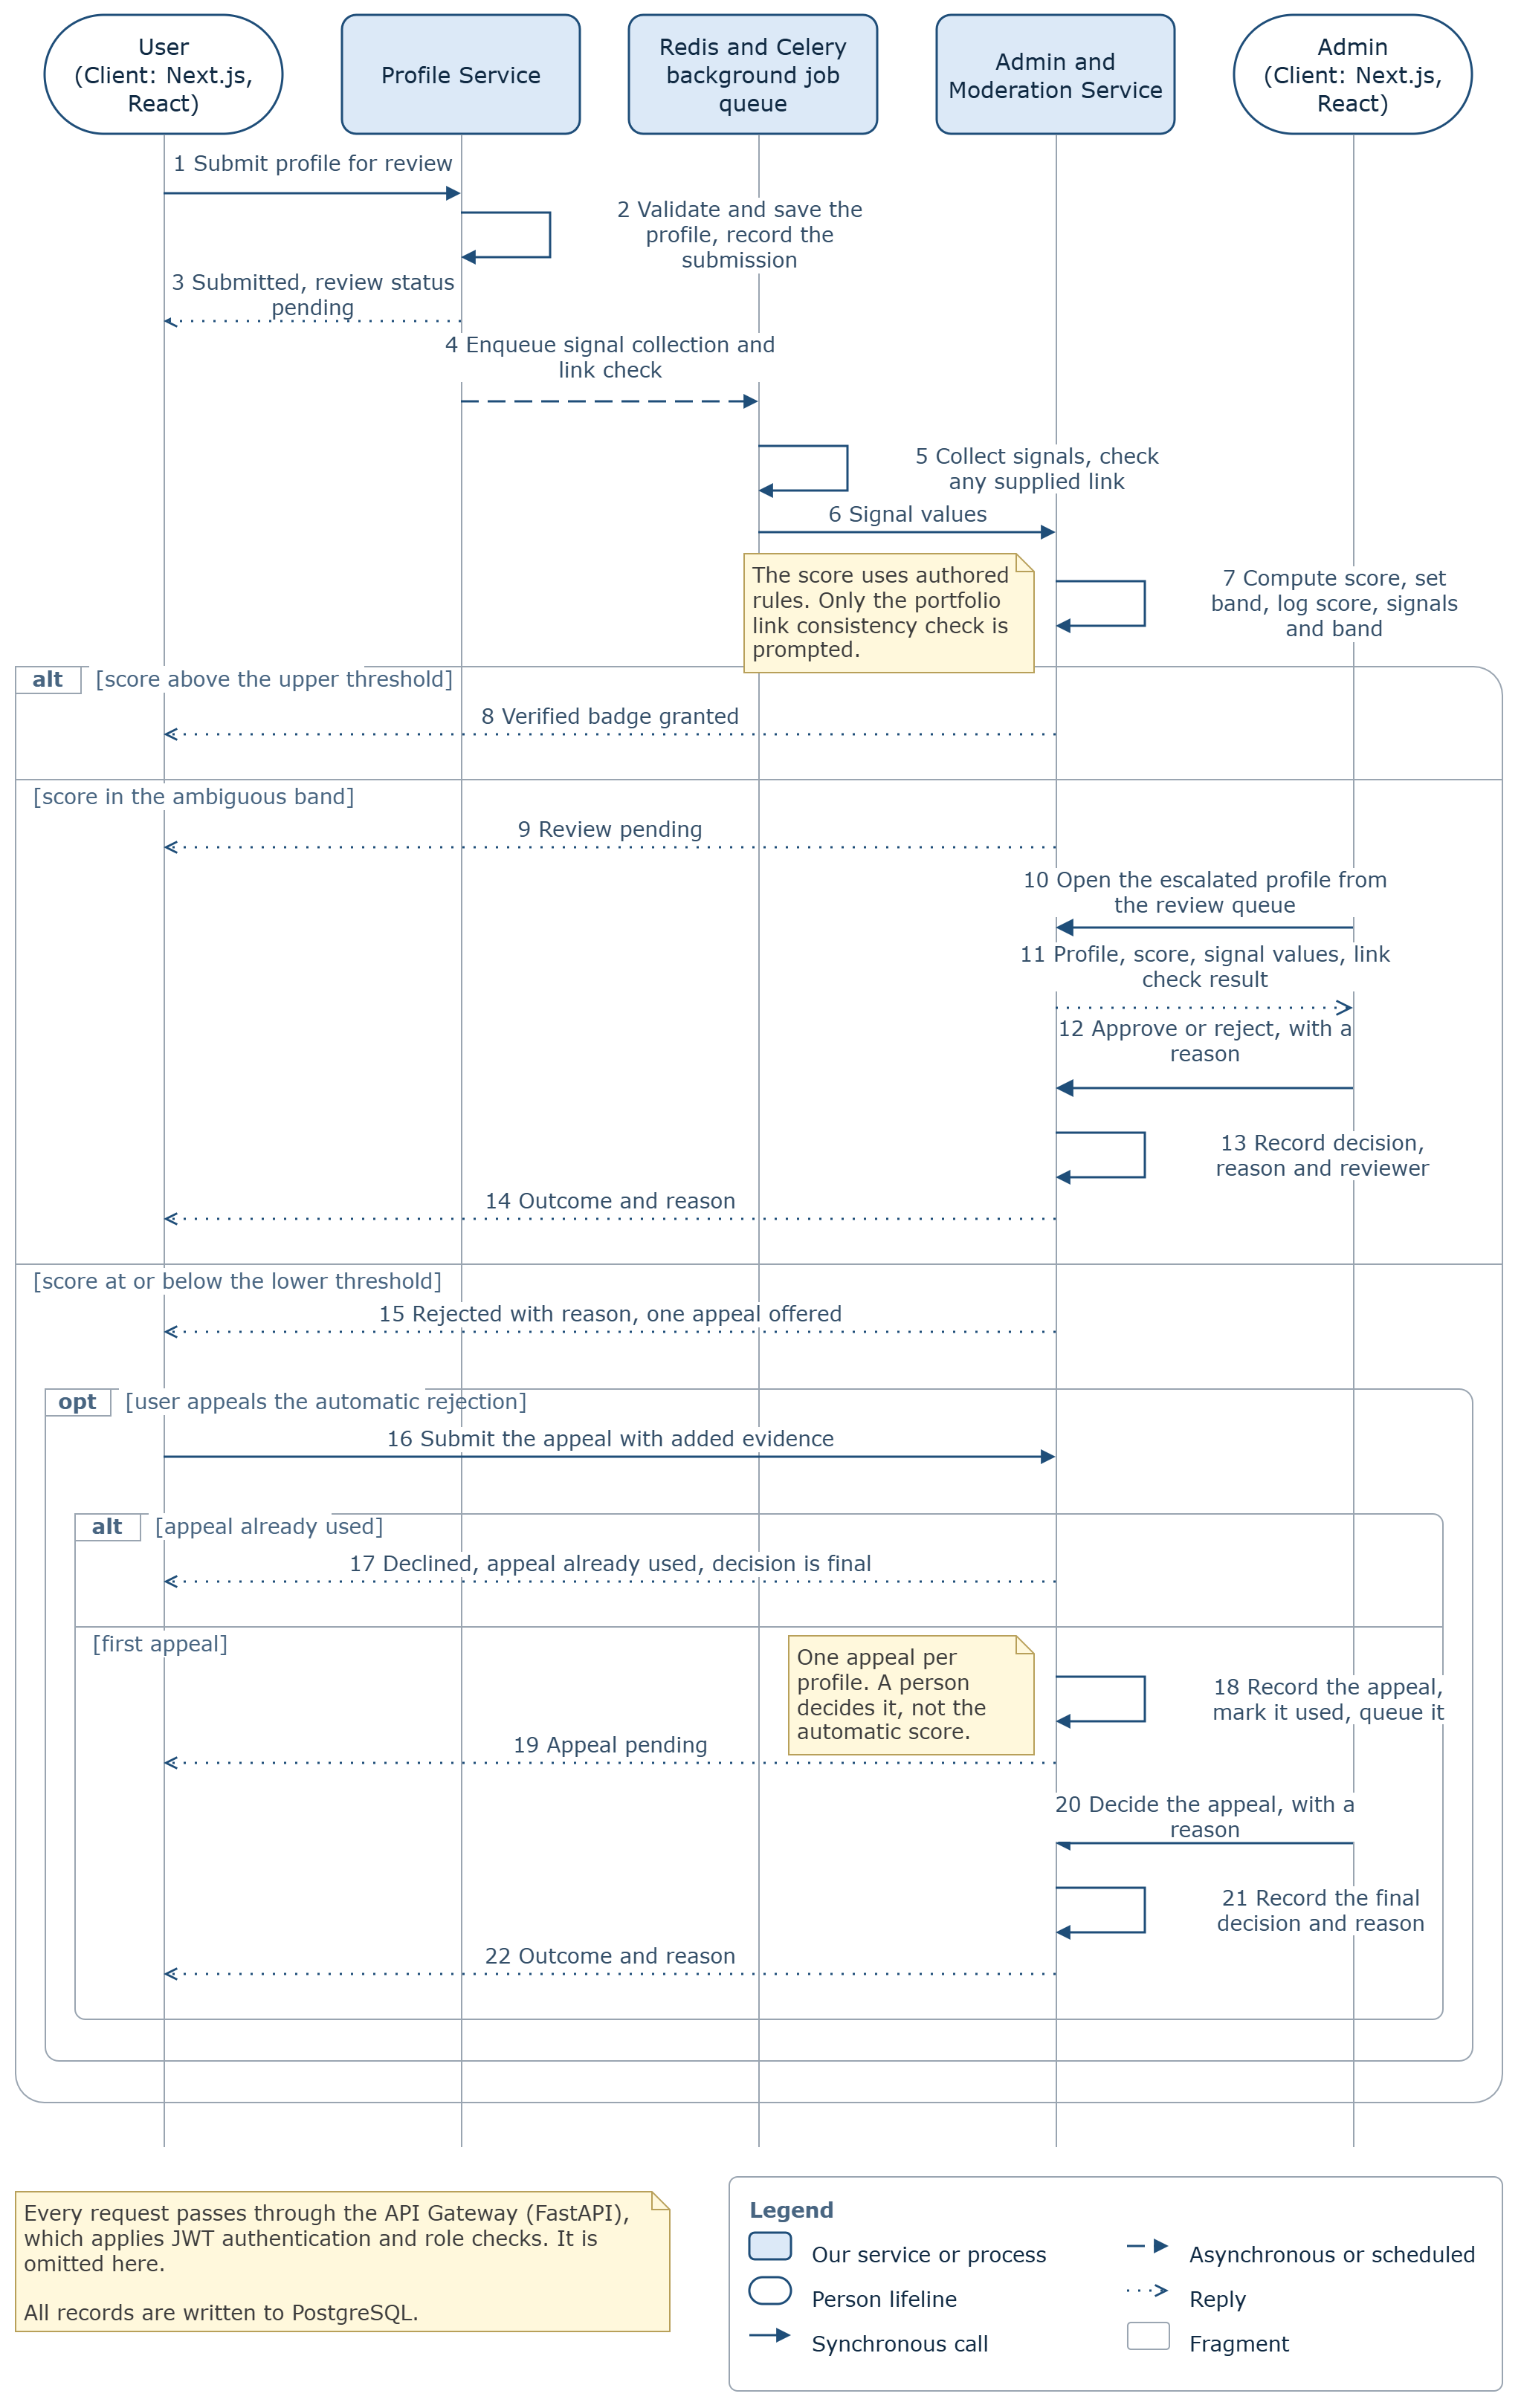
\includegraphics[height=0.6\textheight,keepaspectratio]{Figures/fig21_seq_verification.png}
\caption{Profile verification with escalation and appeal}
\label{fig:seq-verification}
\capdesc{Scores route to verified badge, human review or automatic rejection, and rejection can be appealed.}
\end{figure}

\Needspace{22\baselineskip}
\subsubsection{Match Request and Contact Reveal}

Figure~\ref{fig:seq-match} shows a match request. Ranked results carry no contact details, and both sides see them only after acceptance. In FYP-2 a trained re-ranker replaces the ranking step.

\begin{figure}[H]
\centering
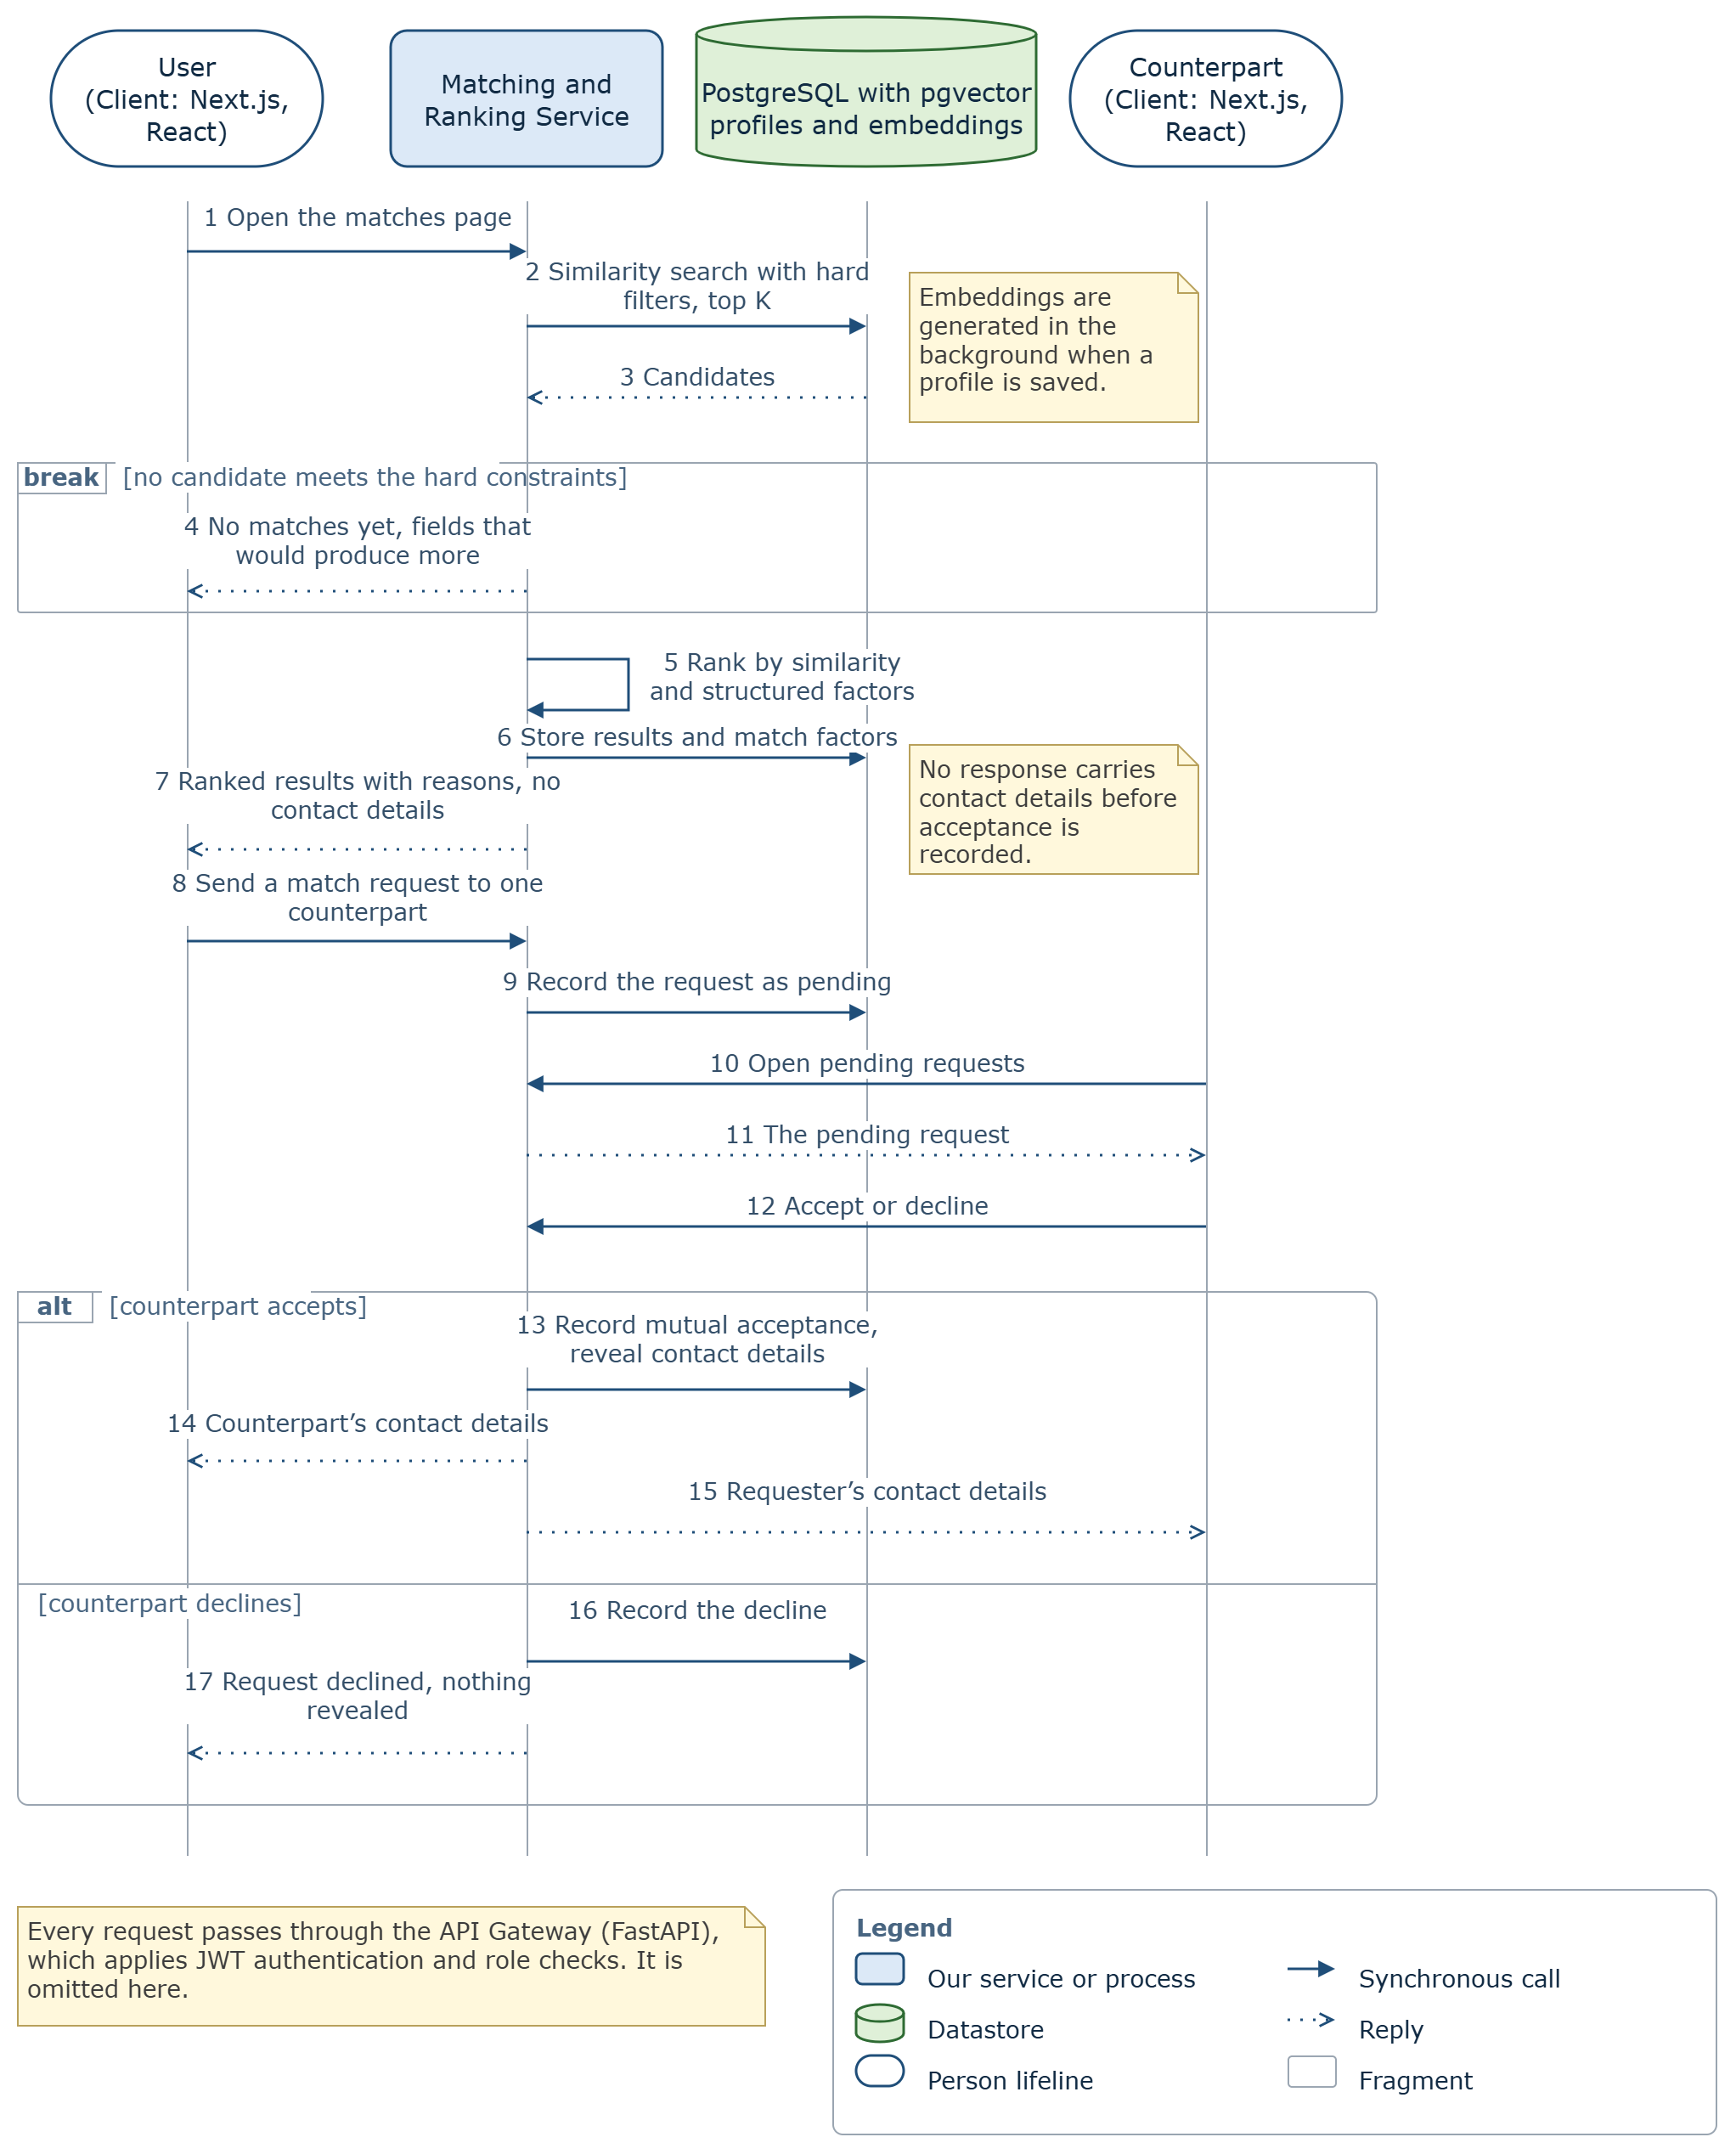
\includegraphics[height=0.6\textheight,keepaspectratio]{Figures/fig22_seq_match.png}
\caption{Match request with mutual acceptance gate}
\label{fig:seq-match}
\capdesc{Ranked matches carry no contact details, which are exchanged only if the counterpart accepts.}
\end{figure}

\Needspace{22\baselineskip}
\subsubsection{Compliance Question with Abstention}

Figure~\ref{fig:seq-compliance} shows a compliance question. The service can abstain after retrieval or after the validation check. The interface says the answer is informational, not legal or tax advice.

\begin{figure}[H]
\centering
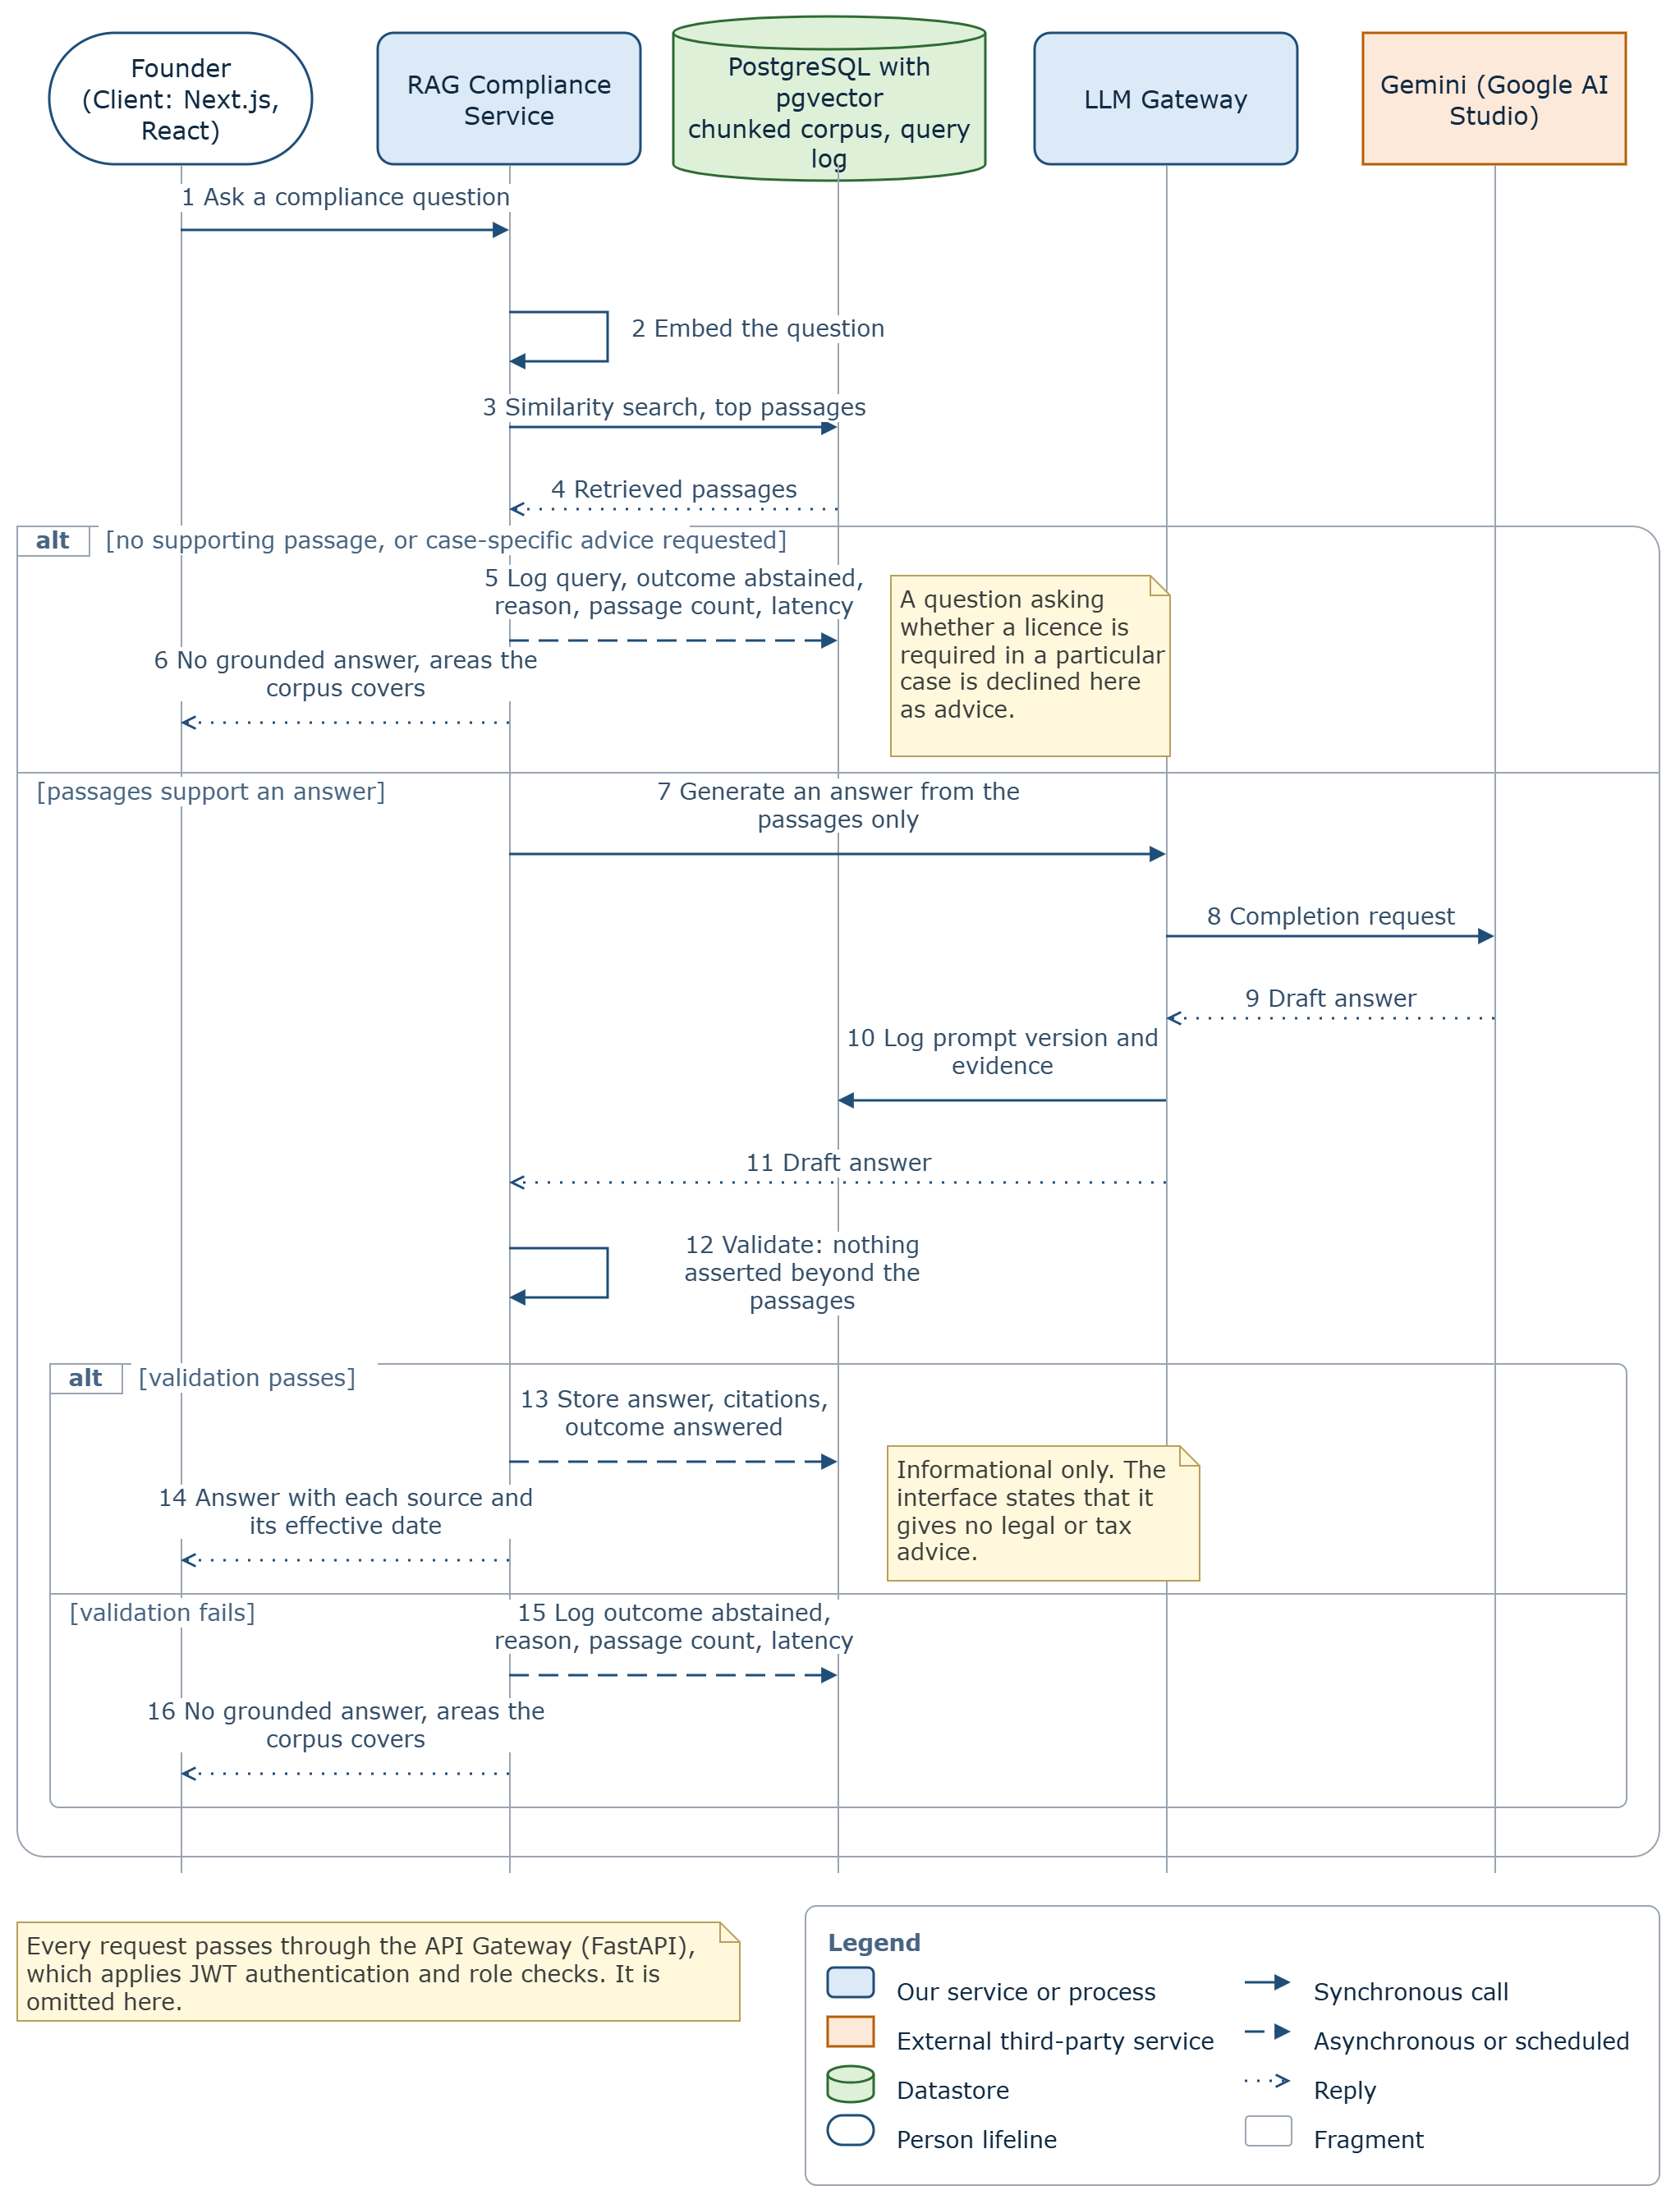
\includegraphics[height=0.6\textheight,keepaspectratio]{Figures/fig23_seq_compliance.png}
\caption{Compliance question flow with abstention}
\label{fig:seq-compliance}
\capdesc{The assistant can abstain after retrieval or after validation, and every outcome is logged.}
\end{figure}

\section{Policies and Tactics}
\label{sec:dbchange}
\begin{itemize}
    \item The project is one repository with four directories: frontend, backend, retrieval (rag) and machine learning (ml). A change across the API boundary is one pull request.
    \item The backend is Python with type annotations and validated request and response models. The frontend is TypeScript.
    \item Both are linted in the pull request pipeline, and a failing run blocks the merge (NFR-23).
    \item Unit tests check scoring and ranking against known inputs.
    \item Integration tests call endpoints with no token, a wrong-role token, and before and after acceptance (NFR-5, NFR-6).
    \item The compliance assistant is tested on a hand-verified gold question set for citations, recall and correct abstention.
    \item Requirement IDs are never renumbered, so the FRs are not contiguous within their groups. Use cases, strategies and tests cite them.
    \item Every schema change is a versioned migration, and the schema rebuilds from an empty database (NFR-22).
    \item Prompts, rubrics and corpus documents are versioned like code. Answers quote the effective date of any fee or rate (NFR-14).
    \item Credentials come from environment configuration, and a pipeline step scans pull requests for API keys (NFR-8).
    \item Provider, model tier, concurrency limits and verification thresholds are configuration values.
    \item Services are container images, and one compose file runs them locally. Deployment from main is planned, with the frontend on Vercel and the backend on Railway or Render.
\end{itemize}

\section{Conclusion}
This chapter described the design of The Founder's Carnet. A Next.js client calls a FastAPI gateway, which passes requests to six services that share one PostgreSQL database, and every model call goes through one LLM gateway. The domain model has 23 classes, and four sequence diagrams cover the main flows. Only the matching re-ranker is a trained model, planned for FYP-2.

\chapter{Conclusions}
This chapter reviews what we did in FYP-1, what we found, where we stand, and what comes next.

\section{Summary of the Work}
The Founder's Carnet is an AI platform where founders, startups, talent, mentors, investors, and an admin role share one reasoning engine. In FYP-1 we have divide problem into 5 parts and add each part to feature. We reviewed nine topics, including six related platforms, and profiled the official documents the compliance assistant will index along with the external datasets. Chapter 4 turned this into requirements, use cases, a database design, and risks, and Chapter 5 gave the architecture.

\section{Findings}
There has been no tarined yet, so these findings come from the literature, our platform audits, and dataset profiling. Our evaluation plan compares any trained model with a simple baseline, as Schein et al. advise. Labels are the main constraint, because we found no public labeled dataset for founder-mentor or investor matching. The re-ranker therefore stays small, with a pilot fallback, and readiness scoring and pitch practice stay as prompted modules. Retrieval alone does not make answers reliable: commercial legal research tools still hallucinated in 17 to 33\% of answers. Our assistant therefore cites its sources and abstains when it cannot support an answer. Official sources sometimes disagree, so we store the effective date of each one. The only Roman Urdu retrieval dataset we found is general search text (Section~\ref{sec:lr-urdu}). We found no audited platform that combines a startup job pathway, a cited compliance assistant, Urdu and Roman Urdu support, and an evaluated matching model.

\section{Scope and Objectives}
Table~\ref{tab:objectives-status} compares each objective of Section~\ref{sec:goals} with what this report delivers and what is left.

\begin{longtable}{|p{0.06\textwidth}|p{0.20\textwidth}|p{0.38\textwidth}|p{0.26\textwidth}|}
\caption{Status of project objectives in this report}
\label{tab:objectives-status}\\[-10pt]
\capdesclt{4}{Delivered and remaining work for each of the nine objectives.}
\hline
\textbf{No.} & \textbf{Objective} & \textbf{Delivered in this report} & \textbf{Remaining} \\ \hline
\endfirsthead
\hline
\textbf{No.} & \textbf{Objective} & \textbf{Delivered in this report} & \textbf{Remaining} \\ \hline
\endhead

1 & One engine for five roles & Architecture, requirements, access rules, use cases, diagrams & Primary user flows by the end of FYP-1 \\ \hline

2 & Cited, abstaining compliance assistant & Design, eleven profiled documents, gold set in preparation & Larger corpus, held-out evaluation \\ \hline

3 & Two-stage matching engine & Design, five factors, cosine baseline, evaluation method & Labels, re-ranker training, baseline comparison \\ \hline

4 & Prompted founder modules & Designs, each with an evaluation approach & Build in the order of Section~\ref{sec:fallback} \\ \hline

5 & Startup pathway for talent & FR-5, FR-6, FR-24, talent screens, job board data model & Build after the pitch simulator and market research \\ \hline

6 & Hybrid profile verification & Scoring rule, three bands, review queue, one appeal, logged decisions & Build with the main flows \\ \hline

7 & English, Urdu, and Roman Urdu benchmark & Literature gap, benchmark design & Run the benchmark, add FR-9 \\ \hline

8 & Narrow legal footprint & No payment between parties, consent first, self-registration only & Legal review before launch \\ \hline

9 & Supporting classifiers & Labels, leakage rules, cleaned datasets & Training and evaluation in FYP-2 \\ \hline

\end{longtable}

\section{Challenges and Limitations}
The most difficult was the matching of the evaluation. There is no public labeled dataset for the Pakistani founder and mentor or investor matching and our initial partner discussion did not result in a partnership, so re-ranker labels will be based on self-registration and a pilot. The legal sources also differ: there are discrepancies between PSEB and FBR/SECP pages, as well as a discrepancy in one of the fee schedules, which was replaced during the project, so each answer is dated. Higher Gemini models were not reliable using free tier load, so we will use Gemini 2.5 or lower, and this is the reason we have the 5 request limit on NFR-2. RAG and multilingual NLP were new to the team (Section \ref{sec:teamexp}) and we started with building the compliance assistant first. We have not trained any model yet, so we make no accuracy claim. The readiness score has not been compared to human reviewers or predicted to be funded, and there has been no review of the fee model by a lawyer or SECP. The FYP-1 build will be English only and will be seeded, billing for placement fees will be handled by FYP-2. Because our datasets are all global or dated (the Pakistani startup census is a snapshot of 2021 and the job postings are ending in March 2021), it is used for informing the schema and profiling process, and the classifiers won't say a thing about any Pakistani startups or resumes. No fairness aware ranking, the Chapter~2 exclusions remain and the 41 table schema might need to be modified once it joins the frontend.

\section{Recommendations and Future Work}

The next step is a partner pilot with an incubator or a few willing mentors and investors, to get real labels and real users. Before launch, a lawyer should review the introduction only boundary and the fee model, and billing should start only after an incorporated entity exists. The corpus also needs upkeep: fee schedules and tax provisions should be reviewed every year, and the Companies Regulations, 2024 should be added. On the technical side, we would try BM25 with reciprocal rank fusion if it improves retrieval on the gold question set, and fine tune embeddings only if the benchmark shows a gap and we have enough labels. Matching fairness needs its own study, with metrics and ethical review.

\section{Plan for FYP-2}
Table~\ref{tab:fyp2-plan} gives the phases, what each depends on, and what closes it.

\begin{longtable}{|p{0.06\textwidth}|p{0.36\textwidth}|p{0.20\textwidth}|p{0.28\textwidth}|}
\caption{Plan for FYP-2}
\label{tab:fyp2-plan}\\[-10pt]
\capdesclt{4}{The six phases of FYP-2, their dependencies, and their exit criteria.}
\hline
\textbf{No.} & \textbf{Work} & \textbf{Depends on} & \textbf{Exit criterion} \\ \hline
\endfirsthead
\hline
\textbf{No.} & \textbf{Work} & \textbf{Depends on} & \textbf{Exit criterion} \\ \hline
\endhead

1 & Close the FYP-1 checkpoint: finish the gold set, expand the corpus, evaluate citations, recall, and abstention & Corpus and gold set & Correct citations and abstention on the held-out set \\ \hline

2 & Matching: collect 150 to 300 labeled pairs, train the re-ranker, compare with the cosine baseline & Partner pilot or seeded users & NDCG@K and MRR against the baseline, or a stated pilot result \\ \hline

3 & Prompted modules: readiness score, pitch simulator, market research, resume optimizer, job board & Profiles and gateway & Readiness score vs. human reviewers on 10 to 15 ideas (Spearman) \\ \hline

4 & Benchmark English, Urdu, and Roman Urdu on 30 to 50 parallel descriptions each, then add FR-9. Train the three supporting classifiers & Phases 1 and 3 & Results per language; macro F1 for each classifier against a simple baseline \\ \hline

5 & Mocked placement fee billing, events calendar, resource links, user manual & Job board & FR-11, FR-30, and FR-31 demonstrated \\ \hline

6 & Load test, usability walkthrough, survey, and founder, talent interviews & All earlier phases & NFR-1, NFR-2, NFR-3, and NFR-16 checked \\ \hline

\end{longtable}

\bibliographystyle{ieeetr}
\bibliography{fypbib}

\appendix
\chapter{Data and Web Sources}
This appendix lists the websites, datasets, platform pages, and official documents the report relies on that are not research papers. The body cites them by the codes in square brackets, for example \src{R1}.

% Allow URLs to break anywhere (symbols, letters, digits) and keep cells ragged-right.
% Column widths are unchanged from the template.
\makeatletter
\g@addto@macro\UrlBreaks{%
  \do\0\do\1\do\2\do\3\do\4\do\5\do\6\do\7\do\8\do\9%
  \do\a\do\b\do\c\do\d\do\e\do\f\do\g\do\h\do\i\do\j\do\k\do\l\do\m%
  \do\n\do\o\do\p\do\q\do\r\do\s\do\t\do\u\do\v\do\w\do\x\do\y\do\z%
  \do\A\do\B\do\C\do\D\do\E\do\F\do\G\do\H\do\I\do\J\do\K\do\L\do\M%
  \do\N\do\O\do\P\do\Q\do\R\do\S\do\T\do\U\do\V\do\W\do\X\do\Y\do\Z%
  \do\-\do\_\do\?\do\=\do\&\do\#\do\:\do\%\do\+\do\,\do\;\do\!\do\(\do\)}
\makeatother
\Urlmuskip=0mu plus 2mu
\newcolumntype{L}[1]{>{\raggedright\arraybackslash}p{#1}}
\setlength{\emergencystretch}{3em}

\section{Ecosystem and market sources}
Table~\ref{tab:src-ecosystem} lists the ecosystem and market sources.

\begin{longtable}{|L{0.07\textwidth}|L{0.30\textwidth}|L{0.34\textwidth}|L{0.19\textwidth}|}
\caption{Ecosystem and market sources}
\label{tab:src-ecosystem}\\[-10pt]
\capdesclt{4}{Code, source, location, and access date of each source in this group.}
\hline
\textbf{Code} & \textbf{Source} & \textbf{Location and notes} & \textbf{Access} \\ \hline
\endfirsthead
\hline
\textbf{Code} & \textbf{Source} & \textbf{Location and notes} & \textbf{Access} \\ \hline
\endhead

P1 & Plan9: Pakistan's First Technology Incubator & \url{https://plan9.pitb.gov.pk/node/1176}. List 14 Cycles and reported 195+ graduated startups & Oct 13, 2026 \\ \hline

P2 & PSEB Annual Report, January--December 2025 & \url{https://techdestination.com/wp-content/uploads/2026/01/Annual-Report-2025-v2-compressed.pdf} & Oct 13, 2026 \\ \hline

P3 & StartupBlink: Global Startup Ecosystem Index 2026 & \url{https://www.startupblink.com/startup-ecosystem/pakistan} & Oct 13, 2026 \\ \hline

P4 & I2I, Pakistan Startup Ecosystem Report 2024 & \url{https://invest2innovate.com/reports/}. 4th edition & Oct 13, 2026 \\ \hline

P5 & Analysing IT Job Market Dynamics in Pakistan & \url{https://doi.org/10.20944/preprints202609.0274.v2}. Preprints.org, v2  & Oct 13, 2026 \\ \hline

\end{longtable}

\section{Platforms and job sites}
Table~\ref{tab:src-platforms} lists the platforms and job sites.

\begin{longtable}{|L{0.07\textwidth}|L{0.30\textwidth}|L{0.34\textwidth}|L{0.19\textwidth}|}
\caption{Platforms and job sites}
\label{tab:src-platforms}\\[-10pt]
\capdesclt{4}{Code, source, location, and access date of each source in this group.}
\hline
\textbf{Code} & \textbf{Source} & \textbf{Location and notes} & \textbf{Access} \\ \hline
\endfirsthead
\hline
\textbf{Code} & \textbf{Source} & \textbf{Location and notes} & \textbf{Access} \\ \hline
\endhead

A1 & I2I, Investor Founder Discovery Platform (IFDP) & \url{https://ifdp.invest2innovate.com} & Oct 03, 2026 \\ \hline

A2 & InnoCollab.pk & \url{https://innocollab.pk} & Audited Sep 2026 \\ \hline

A3 & PakStartups & \url{https://www.pakstartups.org/} & Audited Sep 2026 \\ \hline

A4 & PakLaunch & \url{https://www.paklaunch.com} & Audited Sep 2026 \\ \hline

A5 & StartupNetwork.pk & \url{https://startupnetwork.pk} & Audited Sep 2026 \\ \hline

A6 & Startup.pk & \url{https://startup.pk} & Oct 13, 2026 \\ \hline

A7 & ROZEE.PK, Join a Startup & \url{https://www.rozee.pk/startups} & Oct 13, 2026 \\ \hline

A8 & Indeed, Startup Jobs (keyword search) & \url{https://pk.indeed.com/q-startup-jobs.html} & Oct 13, 2026 \\ \hline

A9 & Glassdoor, Startup Jobs (keyword search) & \url{https://www.glassdoor.com/Job/pakistan-startup-jobs-SRCH_IL.0,8_IN192_KO9,16.htm} & Oct 13, 2026 \\ \hline

\end{longtable}

\section{Datasets}
Table~\ref{tab:src-datasets} lists the datasets.

\begin{longtable}{|L{0.07\textwidth}|L{0.30\textwidth}|L{0.34\textwidth}|L{0.19\textwidth}|}
\caption{Datasets}
\label{tab:src-datasets}\\[-10pt]
\capdesclt{4}{Code, source, location, and access date of each source in this group.}
\hline
\textbf{Code} & \textbf{Source} & \textbf{Location and notes} & \textbf{Access} \\ \hline
\endfirsthead
\hline
\textbf{Code} & \textbf{Source} & \textbf{Location and notes} & \textbf{Access} \\ \hline
\endhead

D1 & Mavkif, Roman-Urdu-Parl-split & \url{https://huggingface.co/datasets/Mavkif/Roman-Urdu-Parl-split}. Hugging Face & Oct 18, 2026 \\ \hline

D2 & Yan Maksi, Startup Success/Fail Dataset from Crunchbase & \url{https://www.kaggle.com/datasets/yanmaksi/big-startup-secsees-fail-dataset-from-crunchbase}. Kaggle & Oct 18, 2026 \\ \hline

D3 & Arindam Banerji, StartUp Investments (Crunchbase) & \url{https://www.kaggle.com/datasets/arindam235/startup-investments-crunchbase}.  Kaggle & Oct 18, 2026 \\ \hline

D4 & Zeeshan Usmani, Pakistan Startup Census (2021) & \url{https://www.kaggle.com/datasets/zusmani/pakistan-startup-census}. Kaggle & Oct 18, 2026 \\ \hline

D5 & Zeeshan Usmani, Pakistan's Job Market (2021) & \url{https://www.kaggle.com/datasets/zusmani/pakistans-job-market}. Kaggle & Oct 18, 2026 \\ \hline

D6 & Snehaan Bhawal, Resume Dataset & \url{https://www.kaggle.com/datasets/snehaanbhawal/resume-dataset}. Kaggle & Oct 18, 2026 \\ \hline

D7 & Haider Maseeh, Resume Dataset & \url{https://www.kaggle.com/datasets/haidermaseeh/resume-dataset}. Kaggle & Oct 18, 2026 \\ \hline

\end{longtable}

\section{Regulatory and legal documents}
Table~\ref{tab:src-regulatory} lists the regulatory and legal documents.

\begin{longtable}{|L{0.07\textwidth}|L{0.30\textwidth}|L{0.34\textwidth}|L{0.19\textwidth}|}
\caption{Regulatory and legal documents}
\label{tab:src-regulatory}\\[-10pt]
\capdesclt{4}{Code, source, location, and access date of each source in this group.}
\hline
\textbf{Code} & \textbf{Source} & \textbf{Location and notes} & \textbf{Access} \\ \hline
\endfirsthead
\hline
\textbf{Code} & \textbf{Source} & \textbf{Location and notes} & \textbf{Access} \\ \hline
\endhead

R1 & FBR, Income Tax Ordinance, 2001 (Updated 30 June, 2026) & \url{https://download1.fbr.gov.pk/Docs/2026724177725705IncomeTaxOrdinanace2001.pdf} & Oct 04, 2026 \\ \hline

R2 & Government of Pakistan, The Finance Act, 2026 & \url{https://download1.fbr.gov.pk/Docs/20266291261044366FinanceAct2026.pdf} & Oct 04, 2026 \\ \hline

R3 & SECP, The Companies Act, 2017 (Updated Aug, 18 2022) & \url{https://www.secp.gov.pk/document/the-companies-act-2017-updated-18-aug-2022/?wpdmdl=45422} & Oct 04, 2026 \\ \hline

R4 & SECP, Seventh Schedule of the Companies Act, 2017: Table of Fees to be Paid to Registrar and Commission & \url{https://www.secp.gov.pk/document/seventh-schedule-updated-till-20-04-2023-2/?wpdmdl=47657} & Oct 04, 2026 \\ \hline

R5 & SECP Regulatory Sandbox Guidelines 2019 & \url{https://www.secp.gov.pk/document/secp-regulatory-sandbox-guidelines-2019/?wpdmdl=37476} & Oct 04, 2026 \\ \hline

R6 & FBR, Information Technology Wing, VOSS for Company Registration & \url{https://download1.fbr.gov.pk/Docs/20194121643945673VirtualOneStopShop(VOSS)forCompanyRegistration.pdf} & Oct 04, 2026 \\ \hline

R7 & FBR, Register for Income Tax & \url{https://www.fbr.gov.pk/categ/register-income-tax/51147/30846/%2071150} & Oct 04, 2026 \\ \hline

R8 & FBR, Registration of Individual on Iris. 25 May 2019 & \url{https://download1.fbr.gov.pk/Docs/2019527755039915Registrationofindividualoniris.pdf} & Oct 04, 2026 \\ \hline

R9 & FBR, Iris -- FAQs & \url{https://e.fbr.gov.pk/SOP/IRIS/Iris_FAQs.pdf} & Oct 04, 2026 \\ \hline

R10 & PSEB, Industry Facilitation and Registration & \url{https://techdestination.com/industry-facilitation/} & Oct 04, 2026 \\ \hline

R11 & National Assembly of Pakistan, PECA, 2016 (Act No. XL of 2016, Sections 4 and 16) & \url{https://nacta.gov.pk/wp-content/uploads/2017/08/Prevention-of-Electronic-Crimes-Act-2016.pdf}. 22 Aug 2016 & Oct 13, 2026 \\ \hline

\end{longtable}

\end{document}